%%% for presentation
\documentclass[pdf,aspectratio=1610]{beamer}

%%% for handouts
%\documentclass[handout,aspectratio=1610]{beamer}
%\usepackage{pgfpages}
%\pgfpagesuselayout{2 on 1}[a4paper,border shrink=20mm]

\usepackage{multimedia}
\usepackage{comment}
\usepackage{amsmath}
\usepackage{amssymb}
\usepackage{amsfonts}
\usepackage{mathptmx}
\usepackage{mathrsfs}
\usepackage{mathtools}
\usepackage{colortbl}
\usepackage{xcolor}
\usepackage[makeroom]{cancel}
\usepackage{wasysym}
\usepackage{svg}
\usepackage[absolute,overlay]{textpos}

% TiKz
\usepackage{tikz,xstring,siunitx,pgfplots,psfrag}
\usetikzlibrary{shapes,arrows,matrix}
\usetikzlibrary{calc,patterns,decorations.pathmorphing,decorations.markings}
\usetikzlibrary{positioning,automata}
\usetikzlibrary{pgfplots.groupplots}
\pgfplotsset{compat=newest}
\tikzstyle{block} = [draw, rectangle, minimum height=2em, minimum width=2em]
\tikzstyle{sum} = [draw, circle, node distance=1.5cm]
\tikzstyle{input} = [coordinate]
\tikzstyle{output} = [coordinate]

\definecolor{DarkGreen}{rgb}{0.087,0.537,0.259}
\definecolor{Maroon}{rgb}{0.550,0.050,0.050}

\newcommand{\TC}[1]{\textcolor{Maroon}{#1}}
\newcommand{\DG}[1]{\textcolor{DarkGreen}{#1}}
\newcommand{\DR}[1]{\textcolor{red!50!black}{#1}}
\newcommand{\DB}[1]{\textcolor{blue!50!black}{#1}}
\newcommand{\MB}[1]{\textcolor{blue!50!green!70!black}{#1}}
\newcommand{\NC}[1]{#1}
\newcommand{\frametitleTC}[1]{\frametitle{\TC{#1}}}
\newcommand{\framesubtitleTC}[1]{\framesubtitle{\TC{#1}}}
\newcommand{\myPause}{\pause}

\newcommand{\red}[1]{\textcolor{red}{#1}}
\newcommand{\blue}[1]{\textcolor{blue}{#1}}
\newcommand{\grn}[1]{\textcolor{DarkGreen}{#1}}
\newcommand{\mgt}[1]{\textcolor{magenta}{#1}}

\newcommand\blfootnote[1]{% footnote w/o marker
  \begingroup
  \renewcommand\thefootnote{}\footnote{#1}%
  \addtocounter{footnote}{-1}%
  \endgroup
}

% \cancel with coloured line
\newcommand{\ccancel}[2][black]{\renewcommand\CancelColor{\color{#1}}\cancel{#2}}   % /
\newcommand{\cbcancel}[2][black]{\renewcommand\CancelColor{\color{#1}}\bcancel{#2}} % \
\newcommand{\cxcancel}[2][black]{\renewcommand\CancelColor{\color{#1}}\xcancel{#2}} % X

% mark a frame containing (only) CC0 images using textpos -- adapt to your aspect ratio &Co.
\setlength{\TPHorizModule}{0.01\textwidth}
\setlength{\TPVertModule}{0.01\textheight}
\textblockorigin{0mm}{0mm}
\setlength{\parindent}{0pt}
\newcommand{\mccz}{\begin{textblock}{5}(112,7){\TC{\small{$^\blacksquare$}}}\end{textblock}}


\mode<presentation>
\beamertemplatenavigationsymbolsempty

\title[PID control for computer engineers]
      {\textcolor{DarkGreen}{\huge{\textbf{PID Control for Computer Engineers}}}}
\subtitle{\textcolor{DarkGreen}{\textbf{with a Systems and Control Theory micro-course in disguise}}}

\author[$\;$A. Leva]
       {\Large{Alberto Leva}\\%
        \small{DEIB, Politecnico di Milano, Italy}\\%
        \small{\texttt{alberto.leva@polimi.it}}
       }

\date{}

\usecolortheme{seagull}
\useoutertheme[subsection=false]{miniframes}
\useinnertheme{circles}
\usefonttheme{professionalfonts}

\setbeamerfont{alerted text}{series=\itshape}
\setbeamercolor{normal text}{fg=darkgray}
\setbeamercolor{alerted text}{fg=blue!40!black}

\setbeamertemplate{footline}
 {
 \begin{beamercolorbox}{section in head/foot}
 \vskip2pt
 \insertshortauthor[width=0.10\textwidth]
 \insertshorttitle[width=0.82\textwidth]
 \insertframenumber / \inserttotalframenumber
 \vskip2pt
 \end{beamercolorbox}
 }

\logo{
\includegraphics[height=3cm]{./logos/PID4CSE-logo.png}}

\begin{document}

{
\setbeamertemplate{headline}{}
\setbeamertemplate{footline}{
  \begin{beamercolorbox}[wd=\paperwidth,ht=2.2ex,dp=1.5ex]{palette quaternary}
  \end{beamercolorbox}
  }
\begin{frame}[noframenumbering]
\titlepage
\end{frame}
}

\section{} % Copyright and licence notes
\begin{frame}[plain,noframenumbering]
 \begin{center}
  \includegraphics[width=0.20\columnwidth]{./CC-BY-SA-icon.png}\\
  \vspace{5mm}\copyright 2019 Alberto Leva\\
  \vspace{5mm}Except where otherwise noted, this work is licensed under a\\
  Creative Commons Attribution-ShareAlike 4.0 International Licence\\
  \vspace{5mm}\texttt{https://creativecommons.org/licenses/by-sa/4.0/}\\
  \vspace{10mm}{\scriptsize
  Creative Commons and the double C in a circle are registered trademarks of Creative Commons
  in the United States and other countries. Third party marks, logos and brands are the property
  of their respective holders.\par
  }   
  \vspace{2mm}{\scriptsize
  Further details and explanations in the copyright and licence notes at the end of this document.\par
  }
 \end{center}
\end{frame}


%%% UNIT 1
{
\setbeamertemplate{headline}{}
\setbeamertemplate{footline}{
  \begin{beamercolorbox}[wd=\paperwidth,ht=2.2ex,dp=1.5ex]{palette quaternary}
  \end{beamercolorbox}
  }
\begin{frame}[noframenumbering]
\frametitle{\DB{\huge{\textbf{$\blacksquare$ Unit 1}}}}
\myPause
 \begin{itemize}
 \item[] \LARGE{\MB{Foreword and prerequisites}}
 \item[] \vspace{-1mm}\LARGE{\MB{Introducing ``control''}}
 \item[] \vspace{-1mm}\LARGE{\MB{Terminology and first examples}}
 \item[] \vspace{-1mm}\LARGE{\MB{A quick visit to the zoo of control}}
 \item[] \vspace{-1mm}\LARGE{\MB{Dynamic systems -- an introduction}}
 \item[] \vspace{-1mm}\LARGE{\MB{Conclusions and discussion}}
 \end{itemize}
\end{frame}
}

\part{}

\section{Foreword and prerequisites}
\subsection{}

\begin{frame}
\frametitleTC{What we are going to do together}
\framesubtitleTC{in a nutshell}
\myPause
\begin{quote}
If you search the literature for ``control in computers'', you will find first that there is a lot of material, and then that the so-called ``PID'' controller is one of the most widely employed.\\
However, as we shall see, an incorrect use of that object can be as disastrous as a good one beneficial. Hence you need to understand and master the underlying principles, that is, the essentials of the systems and feedback control theory.\\
This activity will make you capable in the first place of using PID control knowledgeably, and as a by-product, will also teach you what a dynamic model of a system is.\\
In turn, this is useful for many purposes, including e.g. to detect\\
when a problem cannot be tackled with a PID, and thus you need\\
to learn more control, or ask for advice from a control specialist,\\
or both.
\end{quote}
\end{frame}

\begin{frame}
\frametitleTC{Prerequisites}
\framesubtitleTC{(1/3) mathematics}
\myPause
\begin{itemize}[<+-| alert@+>]
\item Basic knowledge of differential/integral calculus:
      \begin{itemize}[<.(1)->]
      \item limit (finite and infinite),
      \item derivative and integral in one variable.
      \end{itemize}
      \myPause
\item Complex numbers and operations on them.
\item Basic knowledge of matrix algebra:
      \begin{itemize}[<.(1)->]
      \item matrix operations,
      \item determinant, inverse,
      \item eigenvalues and eigenvectors.
      \end{itemize}
\end{itemize}
\end{frame}


\begin{frame}
\frametitleTC{Prerequisites}
\framesubtitleTC{(2/3) physics --- yes we do need a little bit for some examples}
\myPause
\begin{itemize}[<+-| alert@+>]
\item Mass balance: the time derivative of the mass $M$ contained in a volume\\
      (e.g., a tank) is the sum of the $n$ signed mass flowrates $w_i$ at the $n$ boundaries\\
      (e.g., pipes) of that volume, that is,
      \begin{displaymath}
       \frac{dM(t)}{dt} = \sum_{i=1}^n w_i(t).
      \end{displaymath}
\item Energy balance: the time derivative of the energy $E$ contained in a volume\\
      (e.g., a solid body) is the sum of the $n$ signed powers $q_i$ at the $n$\\
      boundaries (e.g., surfaces) of that volume, that is,
      \begin{displaymath}
       \frac{dE(t)}{dt} = \sum_{i=1}^n q_i(t).
      \end{displaymath}
\item We evidently take the convention ``positive means entering''.
\end{itemize}
\end{frame}

\begin{frame}
\frametitleTC{Prerequisites}
\framesubtitleTC{(3/3) physics --- yes we do need a little bit for some examples}
\myPause
\begin{itemize}[<+-| alert@+>]
\item Convective/conductive heat transfer: the power $q_{ab}$ transferred form a body at temperature $T_a$
      to another at temperature $T_b$ is proportional by a \emph{thermal conductance} $G_{ab}$ to the temperature
      difference, that is,
      \begin{displaymath}
       q_{ab}(t) = G_{ab} \left( T_a(t)-T_b(t) \right).
      \end{displaymath}
\item Anticipation: later on we shall see more balances of the \emph{dynamic} type, i.e.,\\
      taking the form``the time derivative of something equals the sum\\
      of something else''.
\item You may be surprised how frequent these are in computing systems,\\
      hence how many different problems can be treated uniformly.
\end{itemize}
\end{frame}


\section{Introducing ``control''}
\subsection{}

\begin{frame}
\frametitleTC{The word ``control'' in the Merriam-Webster dictionary$^*$
              \blfootnote{\small{$^*$\texttt{https://www.merriam-webster.com/dictionary/control}}}}
\framesubtitleTC{(1/3) verb} 
\myPause
\emph{transitive verb}
\begin{tabular}{lll}
 \bf{1} & \bf{a} & archaic: to check, test, or verify by evidence or experiments \\
        & \bf{b} & :to incorporate suitable controls in \\
        &        & \textbf{//} \emph{a controlled experiment} \\
 \bf{2} & \bf{a} & :to exercise restraining or directing influence over: REGULATE \\
        &        & \textbf{//} \emph{control one's anger} \\
        & \bf{b} & :to have power over: RULE \\
        &        & \textbf{//} \emph{A single company controls the industry.} \\
        & \bf{c} & :to reduce the incidence or severity of especially to innocuous levels \\
        &        & \textbf{//} \emph{control an insect population} \\
        &        & \textbf{//} \emph{control a disease} \\
\end{tabular}\\
\vspace{2mm}\emph{intransitive verb}\\
\begin{tabular}{lll}
 :to incorporate controls in an experiment or study -- used with for \\
 \textbf{//} \emph{control for socioeconomic differences}\\
\end{tabular}
\end{frame}

\begin{frame}
\frametitleTC{The word ``control'' in the Merriam-Webster dictionary}
\framesubtitleTC{(2/3) noun} 
\myPause
\begin{tabular}{lll}
 \bf{1} & \bf{a} & :an act or instance of controlling \\
        &        & also: power or authority to guide or manage \\
        &        & \textbf{//} \emph{He took control of the family business.} \\
        & \bf{b} & :skill in the use of a tool, instrument, technique, or artistic medium \\
        &        & \textbf{//} \emph{a singer's control of her voice} \\
        & \bf{c} & :the regulation of economic activity especially by government directive \\
        &        & -- usually used in plural \\
        &        & \textbf{//} \emph{price controls} \\
        &        & \textbf{//} \emph{rent controls} \\
        & \bf{d} & :the ability of a baseball pitcher to control the location of a pitch \\
        &        & within the strike zone \\
 \bf{2} &        & :RESTRAINT, RESERVE \\
        &        & \textbf{//} \emph{exercised control of his passions}
\end{tabular}
\end{frame}

\begin{frame}
\frametitleTC{The word ``control'' in the Merriam-Webster dictionary}
\framesubtitleTC{(3/3) noun, cont'd} 
\myPause
\begin{tabular}{lll}
 \bf{3} & \multicolumn{2}{l}{:one that controls: such as} \\
        & \bf{a} & \textbf{(1)} :an experiment in which the subjects are treated as in a parallel \\
        &        &  experiment except for omission of the procedure or agent under test and which \\
        &        &  is used as a standard of comparison in judging experimental effects\vspace{1mm} \\
        &        & -- called also \emph{control experiment} \\
        &        & \textbf{(2)} :one (such as an organism, culture, or group) that is part of a control \\
        & \bf{b} & a device or mechanism used to regulate or guide the operation of a machine,\\
        &        & apparatus, or system \\
        &        & \textbf{//} \emph{the controls of the aircraft} \\
        & \bf{c} & an organization that directs a spaceflight \\
        &        & \textbf{//} \emph{mission control} \\
        & \bf{d} & a personality or spirit believed to actuate the utterances or\\
        &        & performances of a spiritualist medium \\
 \bf{4} & \multicolumn{2}{l}{or less commonly Control: CONTROL KEY}
\end{tabular}
\end{frame}

\begin{frame}
\frametitleTC{The word is prone to being misunderstood}
\framesubtitleTC{Just a couple of examples} 
\myPause
\begin{itemize}[<+-| alert@+>]
\item Many synonyms (most dangerous ones for us in bold):
      \begin{itemize}
      \item[] bridle, \textbf{check}, constrain, contain, curb, govern, hold, inhibit, \\
              keep, \textbf{measure}, pull in, regulate, rein (in), restrain,\\
              rule, tame,...
      \end{itemize}
\item Many meanings depending on the viewpoint.
\item[] \vspace{-1.5mm}For example, the controls of an aircraft ``regulate or guide'' its operation.
\item[] \vspace{-0.75mm}Fine. So what kind of object/entity do we mean here for ``controls''?
      \begin{itemize}
      \item The knobs, levers and so forth that the pilot manoeuvres?
      \item ...or the autopilot computer with its software?
      \item ...or the ailerons, the rudder and the like?
      \item ...or the compound of all of these?
      \end{itemize}
      \myPause
\item \vfill We definitely need to state our terminology and notation precisely.
\end{itemize}
\end{frame}


\begin{frame}
\frametitleTC{Our definition}
\framesubtitleTC{Take 1 -- for now mostly intuitive, we shall be progressively more precise} 
\myPause
\begin{quote}
 \begin{center}
  \Large{Control is making something behave\\
         as close as possible to how you want it to behave,\\ \myPause
         most often despite there can be other actions besides yours,\\ \myPause
         and also despite you have only a partial knowledge\\
         of the phenomena you are acting upon, \\ \myPause
         hence even the effect of your own actions\\
         may be not entirely predictable.}
 \end{center}
\end{quote}
\end{frame}

\begin{frame}\mccz
\frametitleTC{Why a \underline{theory} for systems and control?}
\framesubtitleTC{} 
\myPause
\begin{quote}
 \begin{center}
  \only<2 | handout:0>{\vspace{-0.4mm}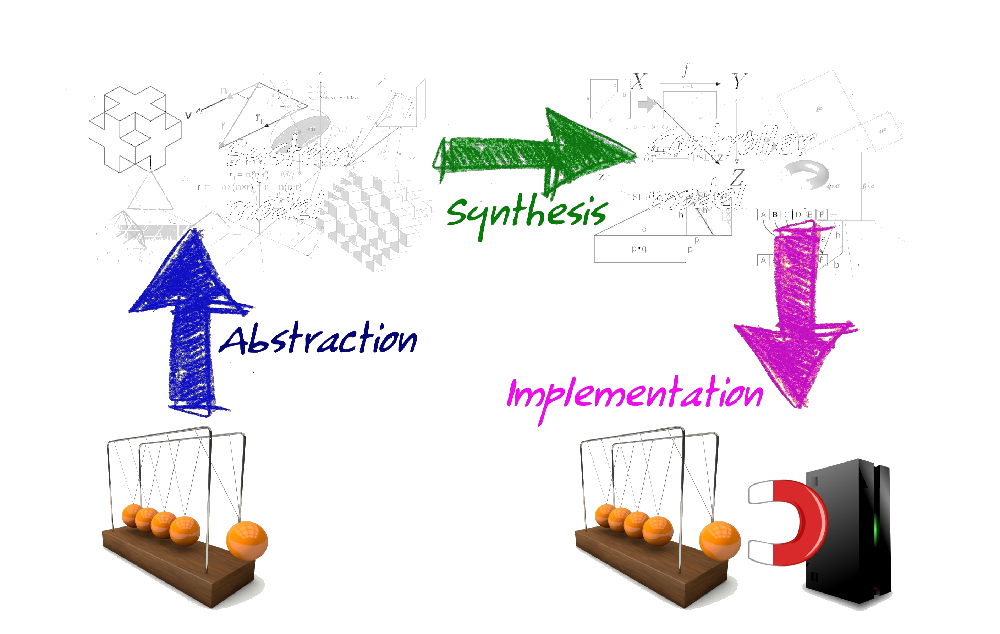
\includegraphics[width=0.85\columnwidth]{./Unit-01/img/RoleOfModels-1_cc0.png}}
  \only<3 | handout:0>{\vspace{-0.4mm}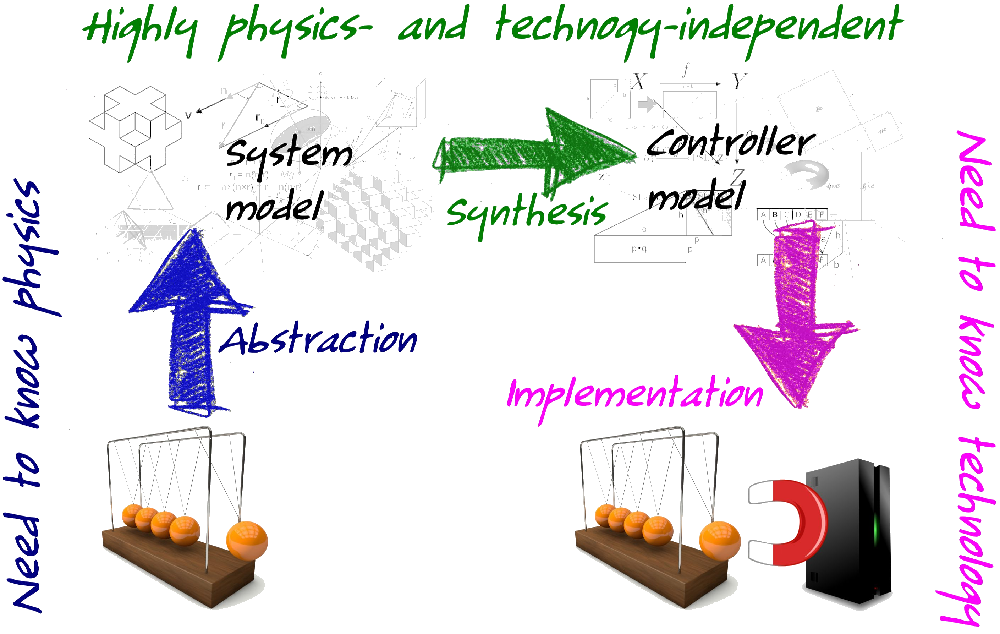
\includegraphics[width=0.85\columnwidth]{./Unit-01/img/RoleOfModels-2_cc0.png}}
  \only<4            >{\vspace{-0.4mm}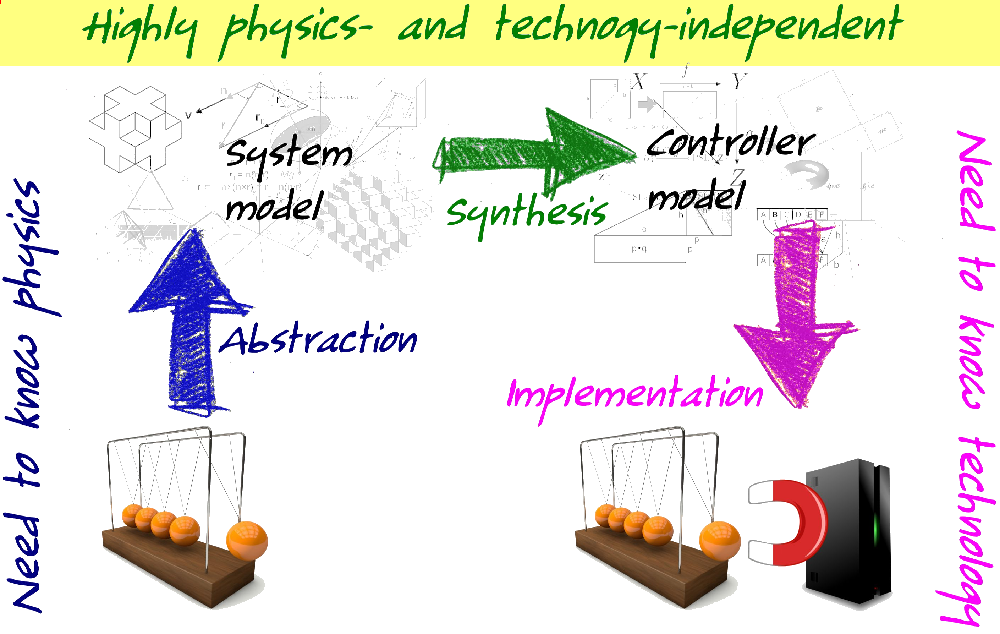
\includegraphics[width=0.85\columnwidth]{./Unit-01/img/RoleOfModels-3_cc0.png}}
 \end{center}
\end{quote}
\end{frame}


\section{Terminology and first examples}
\subsection{}

\begin{frame}
\frametitleTC{Terminology}
\framesubtitleTC{(1/2)}
\myPause
 \begin{itemize}[<+-| alert@+>]
 \item \TC{System} -- when required to avoid ambiguity, \TC{\underline{controlled} system:}
       \begin{itemize}[<+-| alert@+>]
       \item[] the object or phenomenon to be governed
       \item[] (a vehicle, the thermal behaviour of a building,...).
       \end{itemize}
 \item \TC{Requirements} or \TC{objectives:}
       \begin{itemize}[<+-| alert@+>]
       \item[] what you want the system to do\\
       \item[] (cruise as close as possible to 50 km/h, keep temperature between 18$^{\circ}$C\\
                and 21$^{\circ}$C in all rooms,...)
       \end{itemize}
 \item \TC{Controls} or \TC{control actions} or simply \TC{actions:}
       \begin{itemize}[<+-| alert@+>]
       \item[] what is done to the system with the purpose of fulfilling the requirements
       \item[] (act on the gas/brakes, modulate fuel flowrate to heater,\\
                operate fan coils,...).
       \end{itemize}
 \item \TC{Outcomes:}
       \begin{itemize}[<+-| alert@+>]
       \item[] the actual behaviour of the system
       \item[] (real speed and temperature behaviour over time,...).
       \end{itemize}
 \end{itemize}
\end{frame}

\begin{frame}
\frametitleTC{Terminology}
\framesubtitleTC{(2/2)}
\myPause
 \begin{itemize}[<+-| alert@+>]
 \item \TC{Disturbances:}
       \begin{itemize}[<+-| alert@+>]
       \item[] anything that affects the outcomes and cannot be manipulated, but possibly sensed
       \item[] (road slope, wind, vehicle load, weather, room occupancy,...);
       \item[] in other words, actions from the environment to which the system must be resilient.
       \end{itemize}
 \item \TC{Sensors:}
       \begin{itemize}[<+-| alert@+>]
       \item[] the entities that gather information from the system
       \item[] (tacho/accelerometer, GPS, inside/outside temperature sensors,...).
       \end{itemize}
 \item \TC{Actuators:}
       \begin{itemize}[<+-| alert@+>]
       \item[] the entities that act on the system to exert the actions
       \item[] (engine, brakes, burners, pumps, valves,...).
       \end{itemize}
 \item \TC{Controllers:}
       \begin{itemize}[<+-| alert@+>]
       \item[] the entities that determine the actions given the information\\
               deemed relevant\\
       \item[] (the object of your design).
       \end{itemize}
 \end{itemize}
\end{frame}

\begin{frame}
\frametitleTC{Remarks}
\framesubtitleTC{}
\myPause
 \begin{itemize}[<+-| alert@+>]
 \item Quite often we can talk about a control \TC{objective} in terms of a \TC{signal}\\
       following another one.
 \item In the case we use to say that
       \begin{itemize}[<+-| alert@+>]
       \item we have a \TC{controlled variable} (e.g., the speed of a vehicle)
       \item and want it to follow a \TC{set point} or \TC{reference} signal (e.g., go from 0 to 100 km/h
             linearly in 10 seconds).
       \end{itemize}
 \item Also, quite often our action can be viewed as setting a variable (e.g., the gas\\
       valve opening in the 0--100\% range); we call such a variable\\
       the \TC{control signal}.
 \item Consistently, we can often represent exogenous actions (e.g., wind\\
       speed and directions) that we called \TC{disturbances}, as signals.
 \end{itemize}
\end{frame}

\begin{frame}
\frametitleTC{Remarks}
\framesubtitleTC{}
\myPause
 \begin{itemize}[<+-| alert@+>]
 \item You are probably thinking that in the computer world the situation just sketched is hardly ever encountered.
 \item The objection seems in fact reasonable, as the entities one manages in computers are far more
       heterogeneous than mere numbers varying over time.
 \item \vfill Nonetheless hold on; you will discover that on the contrary, much more computer-related problems
       than one expects, can be formulated in terms\\ of \TC{set point following} and/or \TC{disturbance rejection}.
 \item In the end, learning systems and control is learning a new kind\\
       of abstraction.
 \end{itemize}
\end{frame}



\section{The control zoo}
\subsection{}

\begin{frame}\mccz
\frametitleTC{A first, quick visit to the zoo of control}
\myPause
 \begin{columns}
  \column[T]{0.20\textwidth}
   \only<2->{
\includegraphics[height=6cm]{./Unit-01/img/ZenWhale_cc0.jpg}}
  \column[T]{0.70\textwidth}
   \begin{quote}
    \begin{small}
     \onslide<3->{Now the various species of whales need some sort of popular comprehensive classification,
                  if only an easy outline one for the present, hereafter to be filled in all its departments
                  by subsequent labourers. As no better man advances to take this matter in hand, I hereupon
                  offer my own poor endeavours.\\
                  I promise nothing complete; because any human thing supposed to be complete, must for that
                  very reason infallibly be faulty. I shall not pretend to a minute anatomical description
                  of the various species, or -- in this place at least -- to much of any description.\\
                  My object here is simply to project the draught\\
                  of a systematisation of Cetology. I am the\\
                  architect, not the builder.\\
                  \vspace{1mm}$\qquad\qquad\qquad\;\;\;\;$H. Melville, Moby Dick, XXXII
                  }
    \end{small}
   \end{quote}
 \end{columns}
\end{frame}

\begin{frame}
\frametitleTC{A very simple control taxonomy -- axis 1}
\framesubtitleTC{What information is used by the controller (sensors and actuators not drawn for simplicity)}
\myPause
 \begin{itemize}[<+-| alert@+>]
 \item Requirements and possibly disturbances\\
       $\Rightarrow$ \TC{open-loop} control, possibly with \TC{disturbance compensation}:
       \begin{center}
        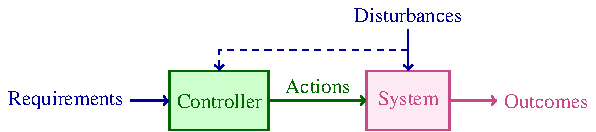
\includegraphics[width=0.60\columnwidth]{./Unit-01/img/Taxonomy-OpenLoop-scheme.pdf}
       \end{center}
 \item Requirements, \underline{system output(s)} and possibly disturbances\\
       $\Rightarrow$ \TC{closed-loop} or \TC{feedback} control, possibly with \TC{disturbance compensation}:
       \begin{center}
        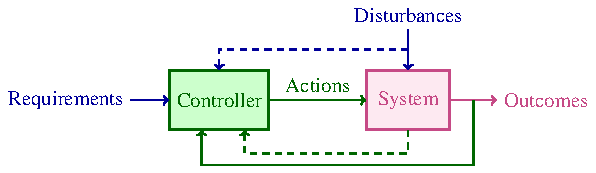
\includegraphics[width=0.60\columnwidth]{./Unit-01/img/Taxonomy-ClosedLoop-scheme.pdf}
       \end{center}
 \end{itemize}
\end{frame}

\begin{frame}\mccz
\frametitleTC{A very simple control taxonomy -- axis 2}
\framesubtitleTC{When the controller determines the control action}
\myPause
 \begin{columns}
  \column[T]{0.25\textwidth}
   \only<2 | handout:0>{\centering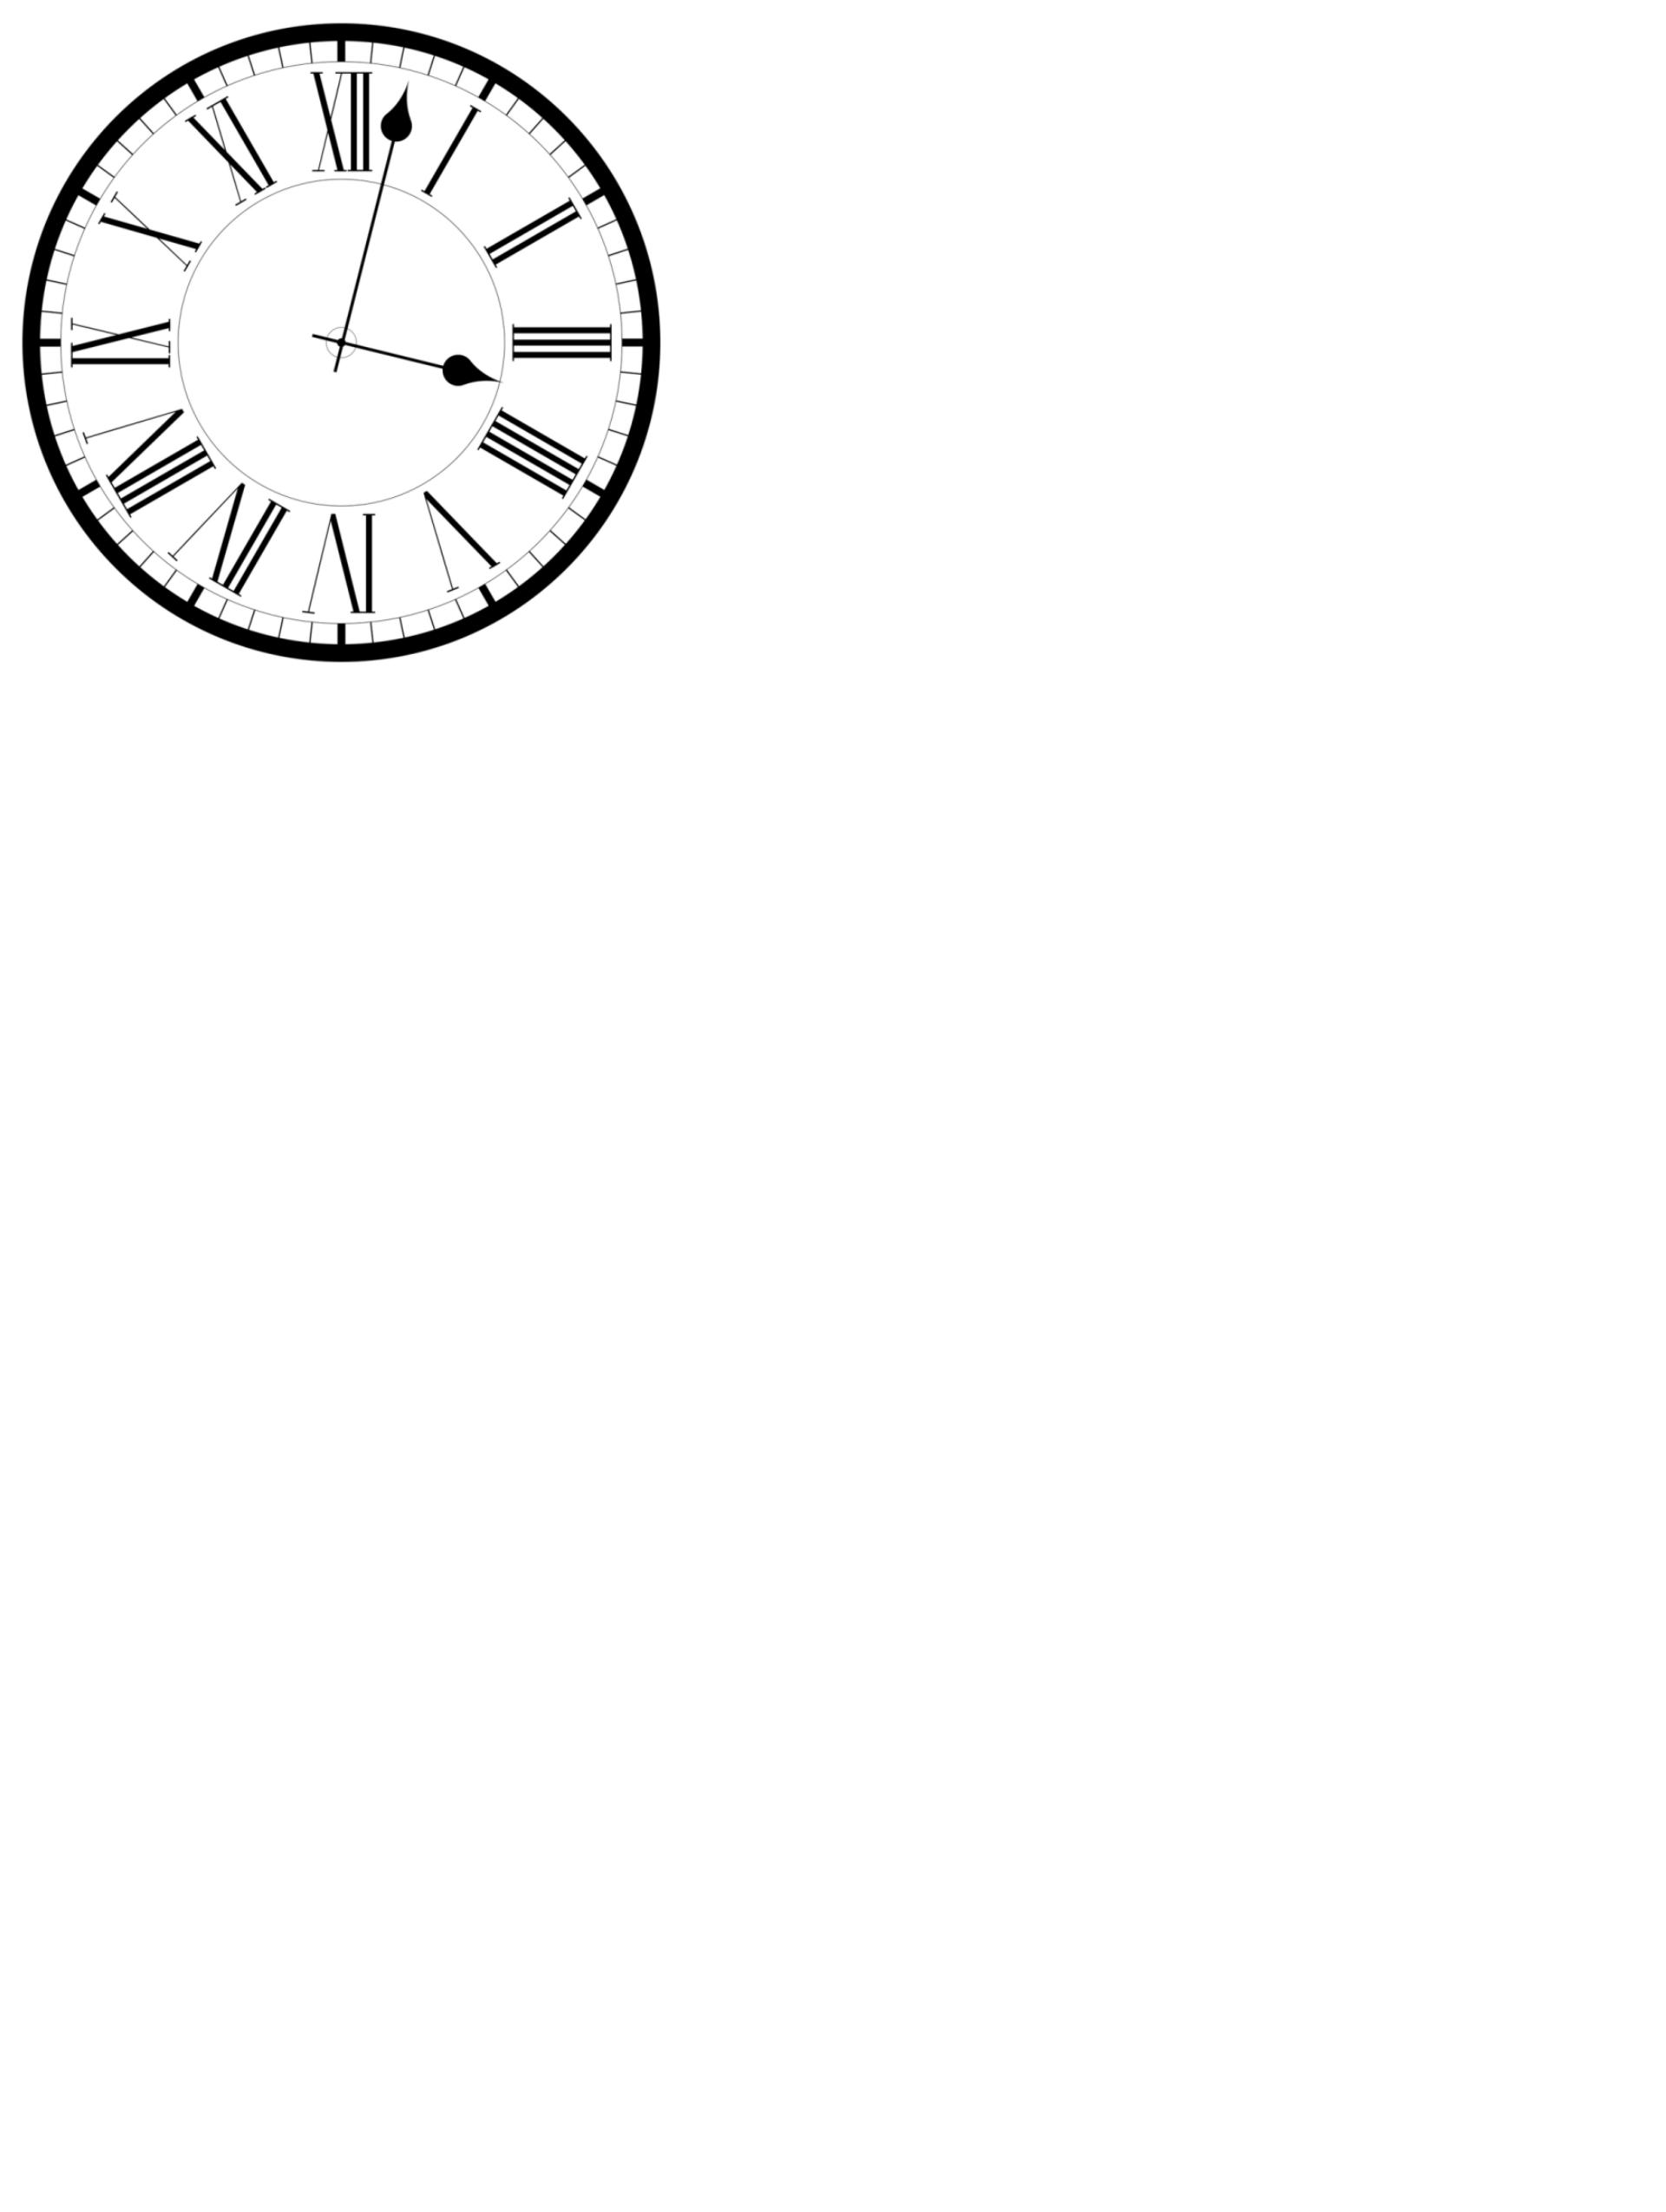
\includegraphics[height=5.5cm]{./Unit-01/img/Taxonomy-When-1_cc0.jpg}}%
   \only<3 | handout:0>{\centering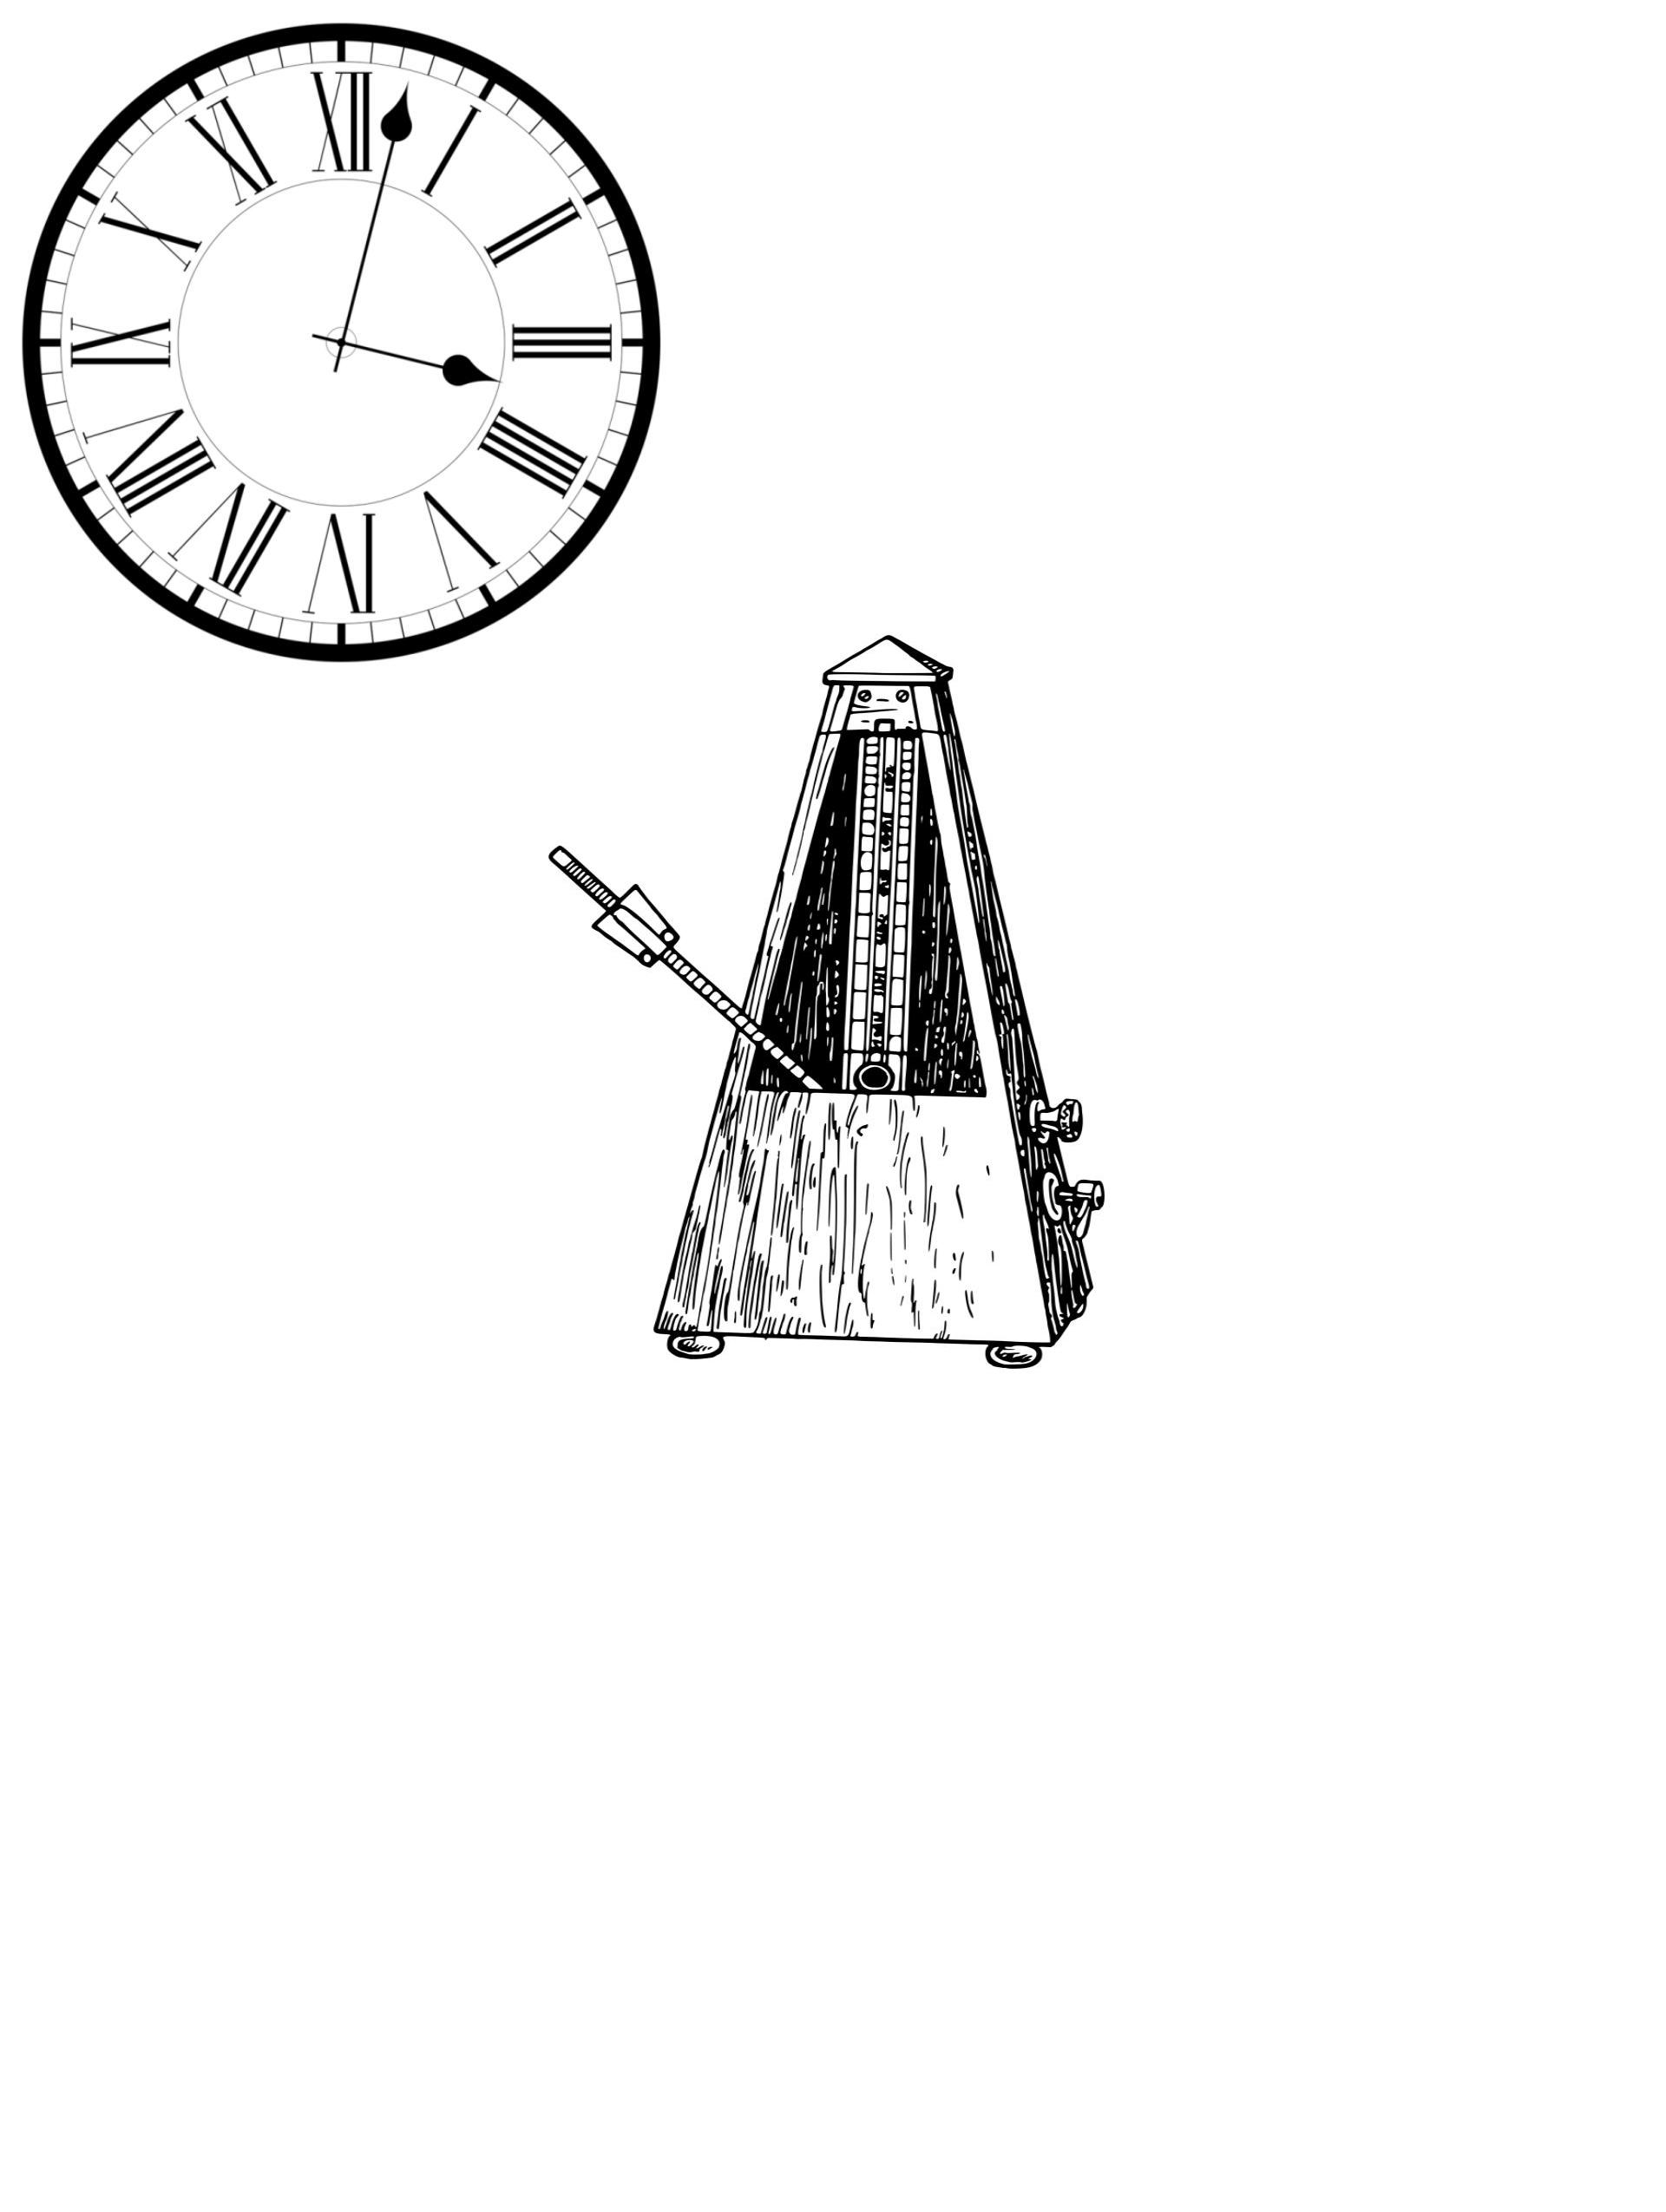
\includegraphics[height=5.5cm]{./Unit-01/img/Taxonomy-When-2_cc0.jpg}}%
   \only<4-           >{\centering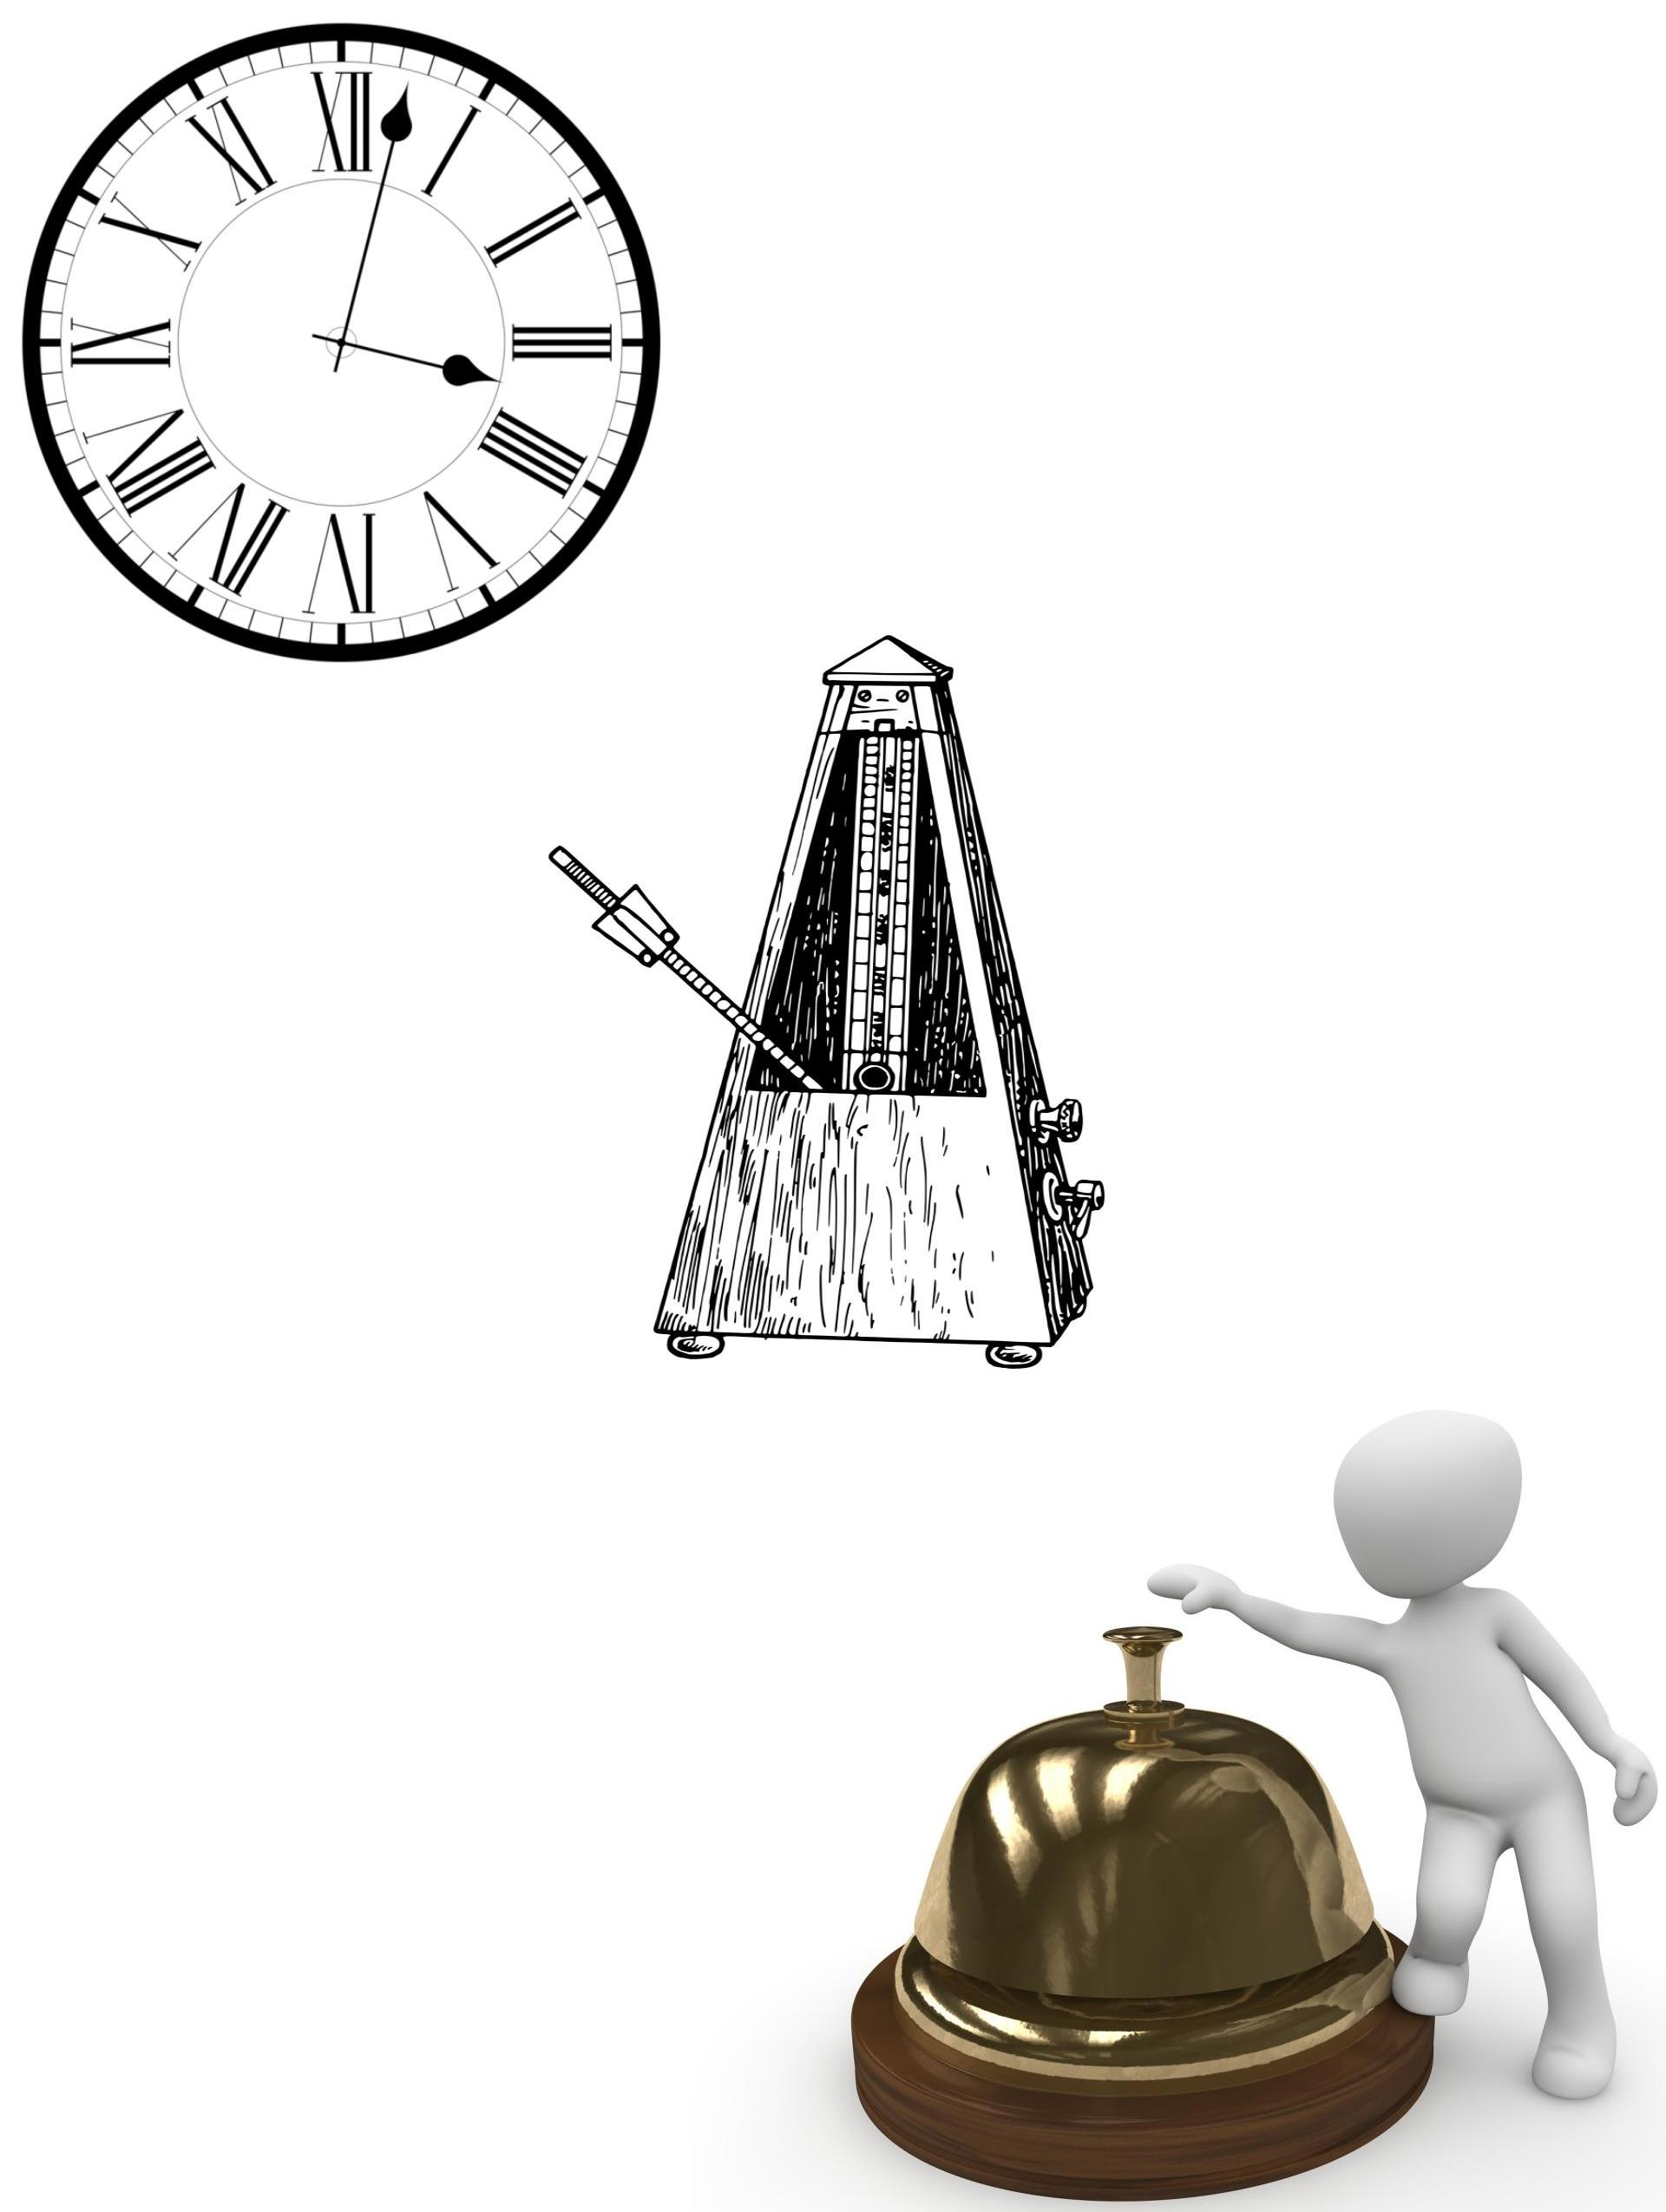
\includegraphics[height=5.5cm]{./Unit-01/img/Taxonomy-When-3_cc0.jpg}}%
  \column[T]{0.70\textwidth}
   \begin{itemize}[<+-| alert@+>]
   \item Continuously $\Rightarrow$ \TC{continuous-time} control\\
         (e.g., analogue electronics).
   \item \vspace{6mm}At points in time known \emph{a priori} $\Rightarrow$ \TC{discrete-time} control\\
         (e.g. and most typical, ISR for a \TC{periodic} interrupt).
   \item \vspace{6mm}When requested $\Rightarrow$ \TC{event-triggered} control\\
         (e.g., when a signal has changed 
          by more\\ than a given quantity wrt the last\\ control determination).
   \end{itemize}
 \end{columns}
\end{frame}

\begin{frame}\mccz
\frametitleTC{A very simple control taxonomy -- axis 3}
\framesubtitleTC{What is the nature of the control action}
\myPause
 \begin{columns}
  \column[T]{0.25\textwidth}
   \only<2 | handout:0>{\centering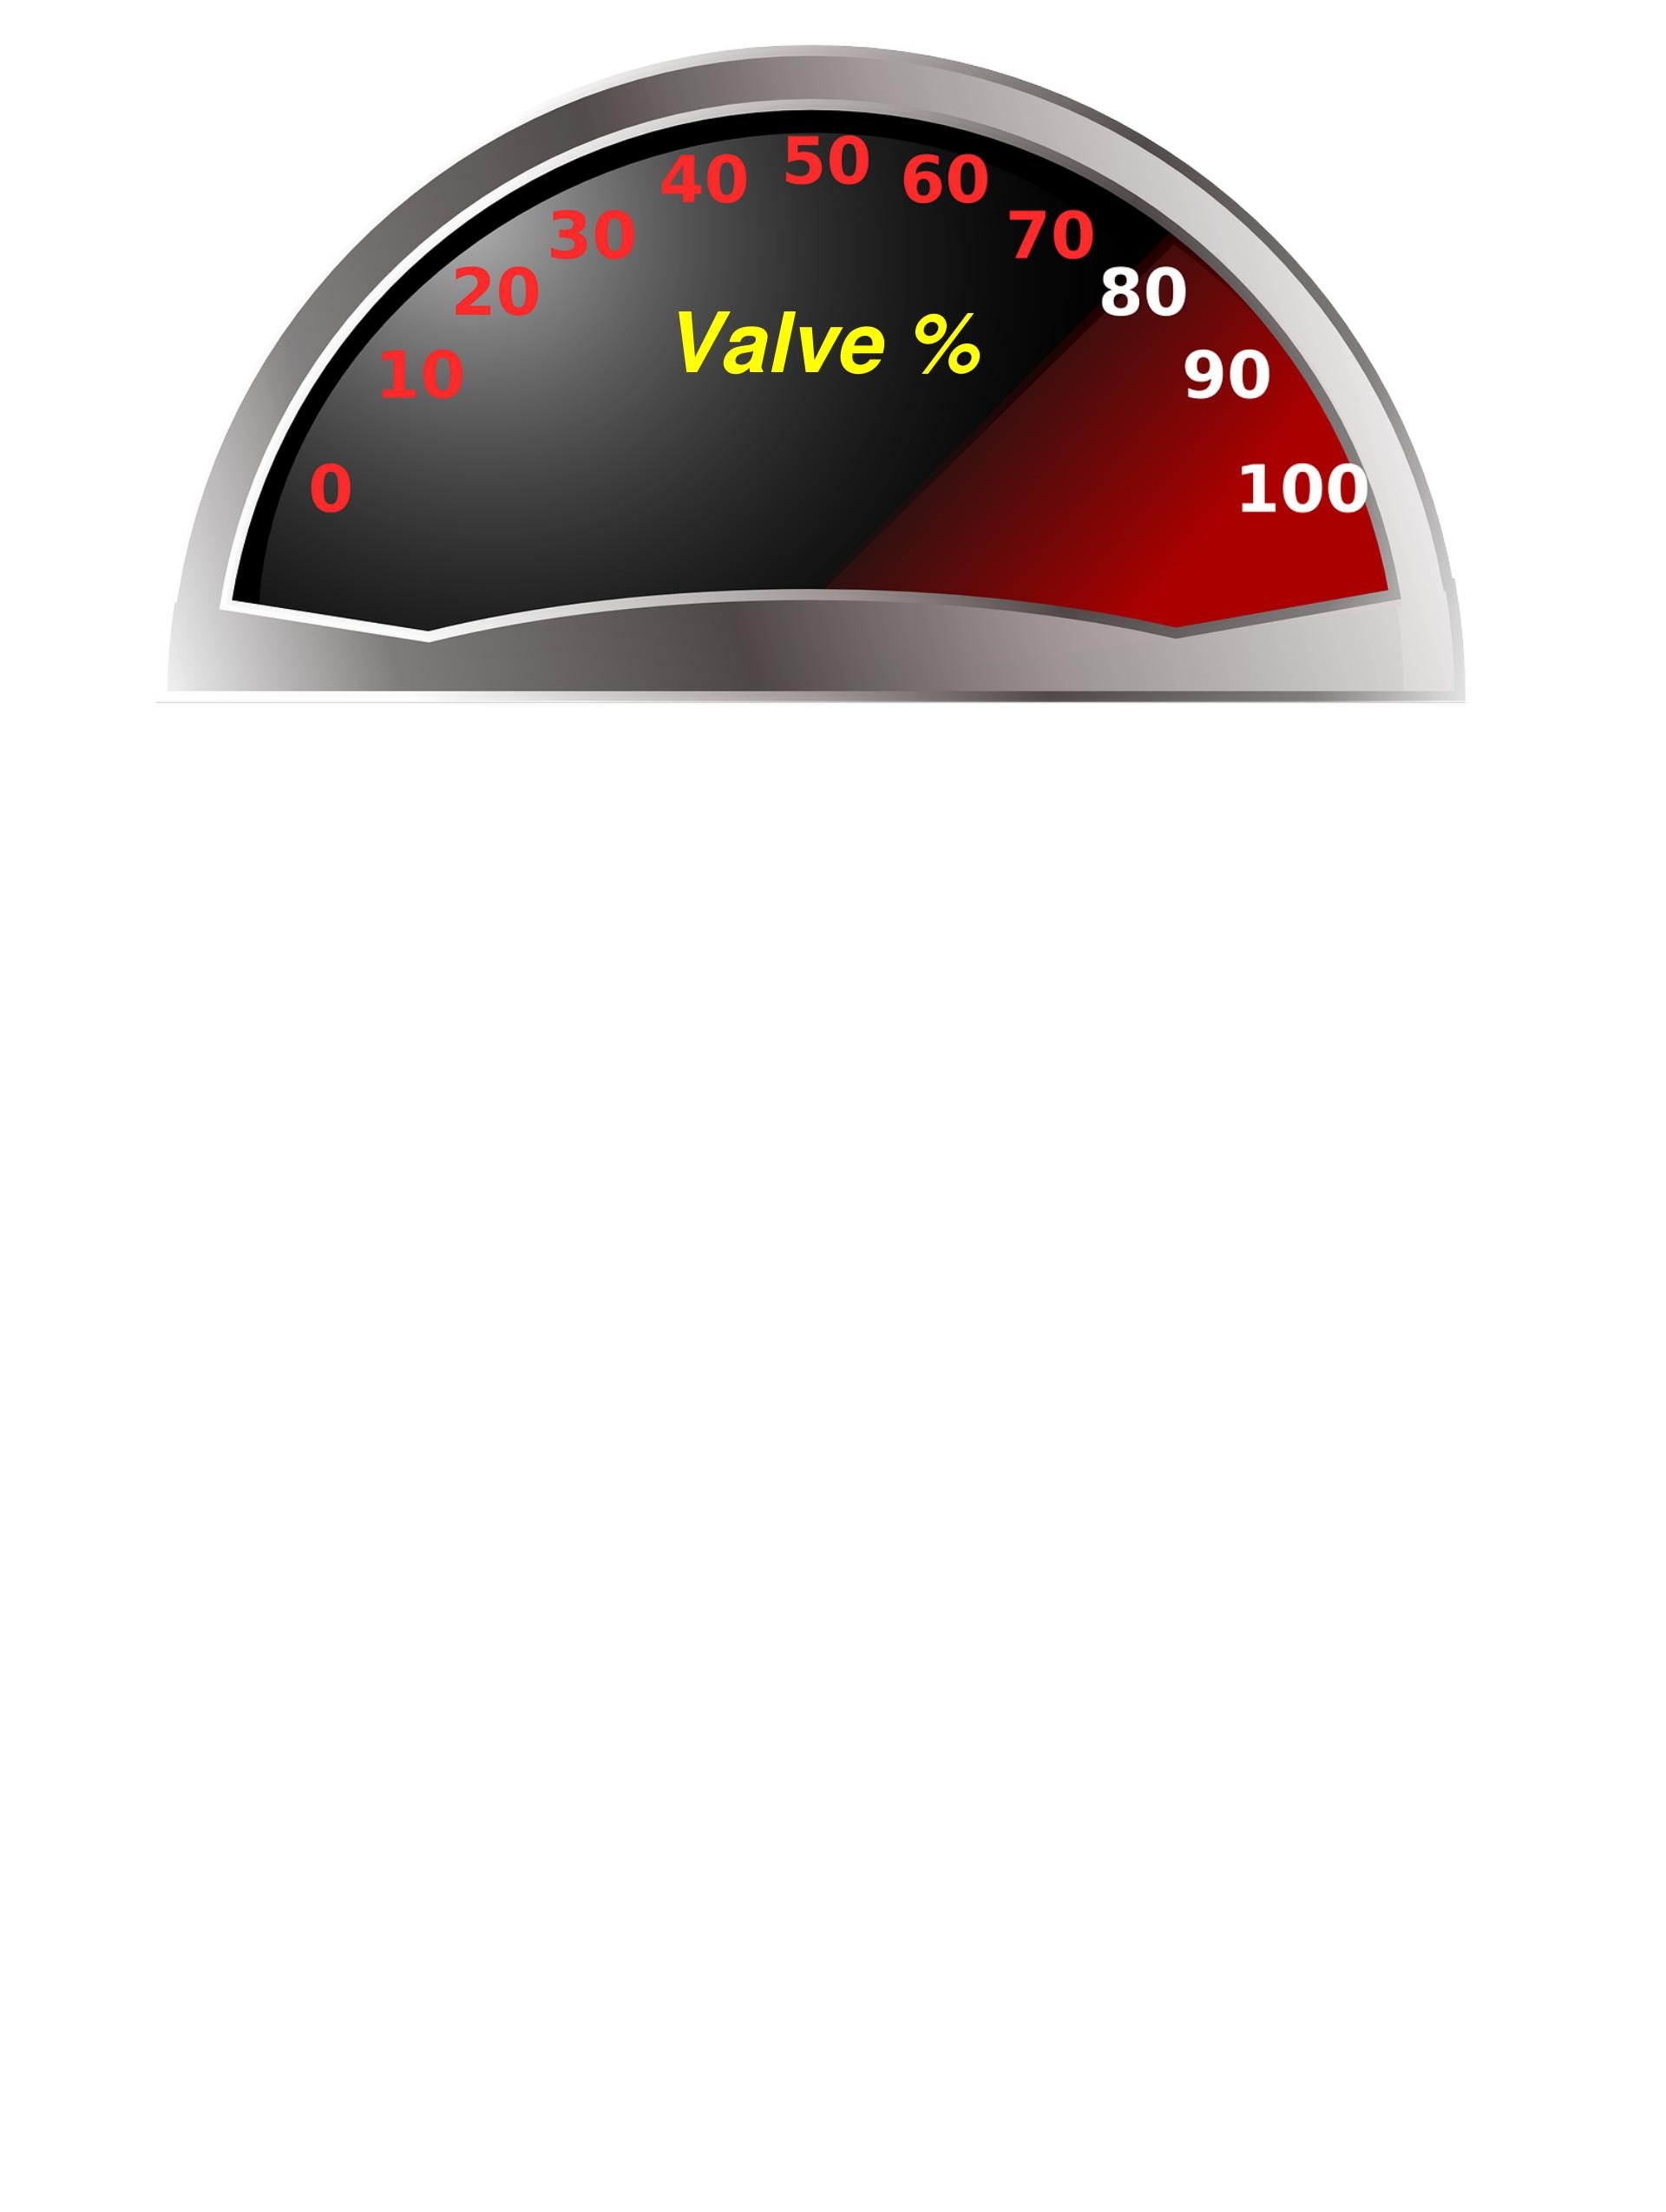
\includegraphics[height=6cm]{./Unit-01/img/Taxonomy-MvsL-1_cc0.jpg}}%
   \only<3-           >{\centering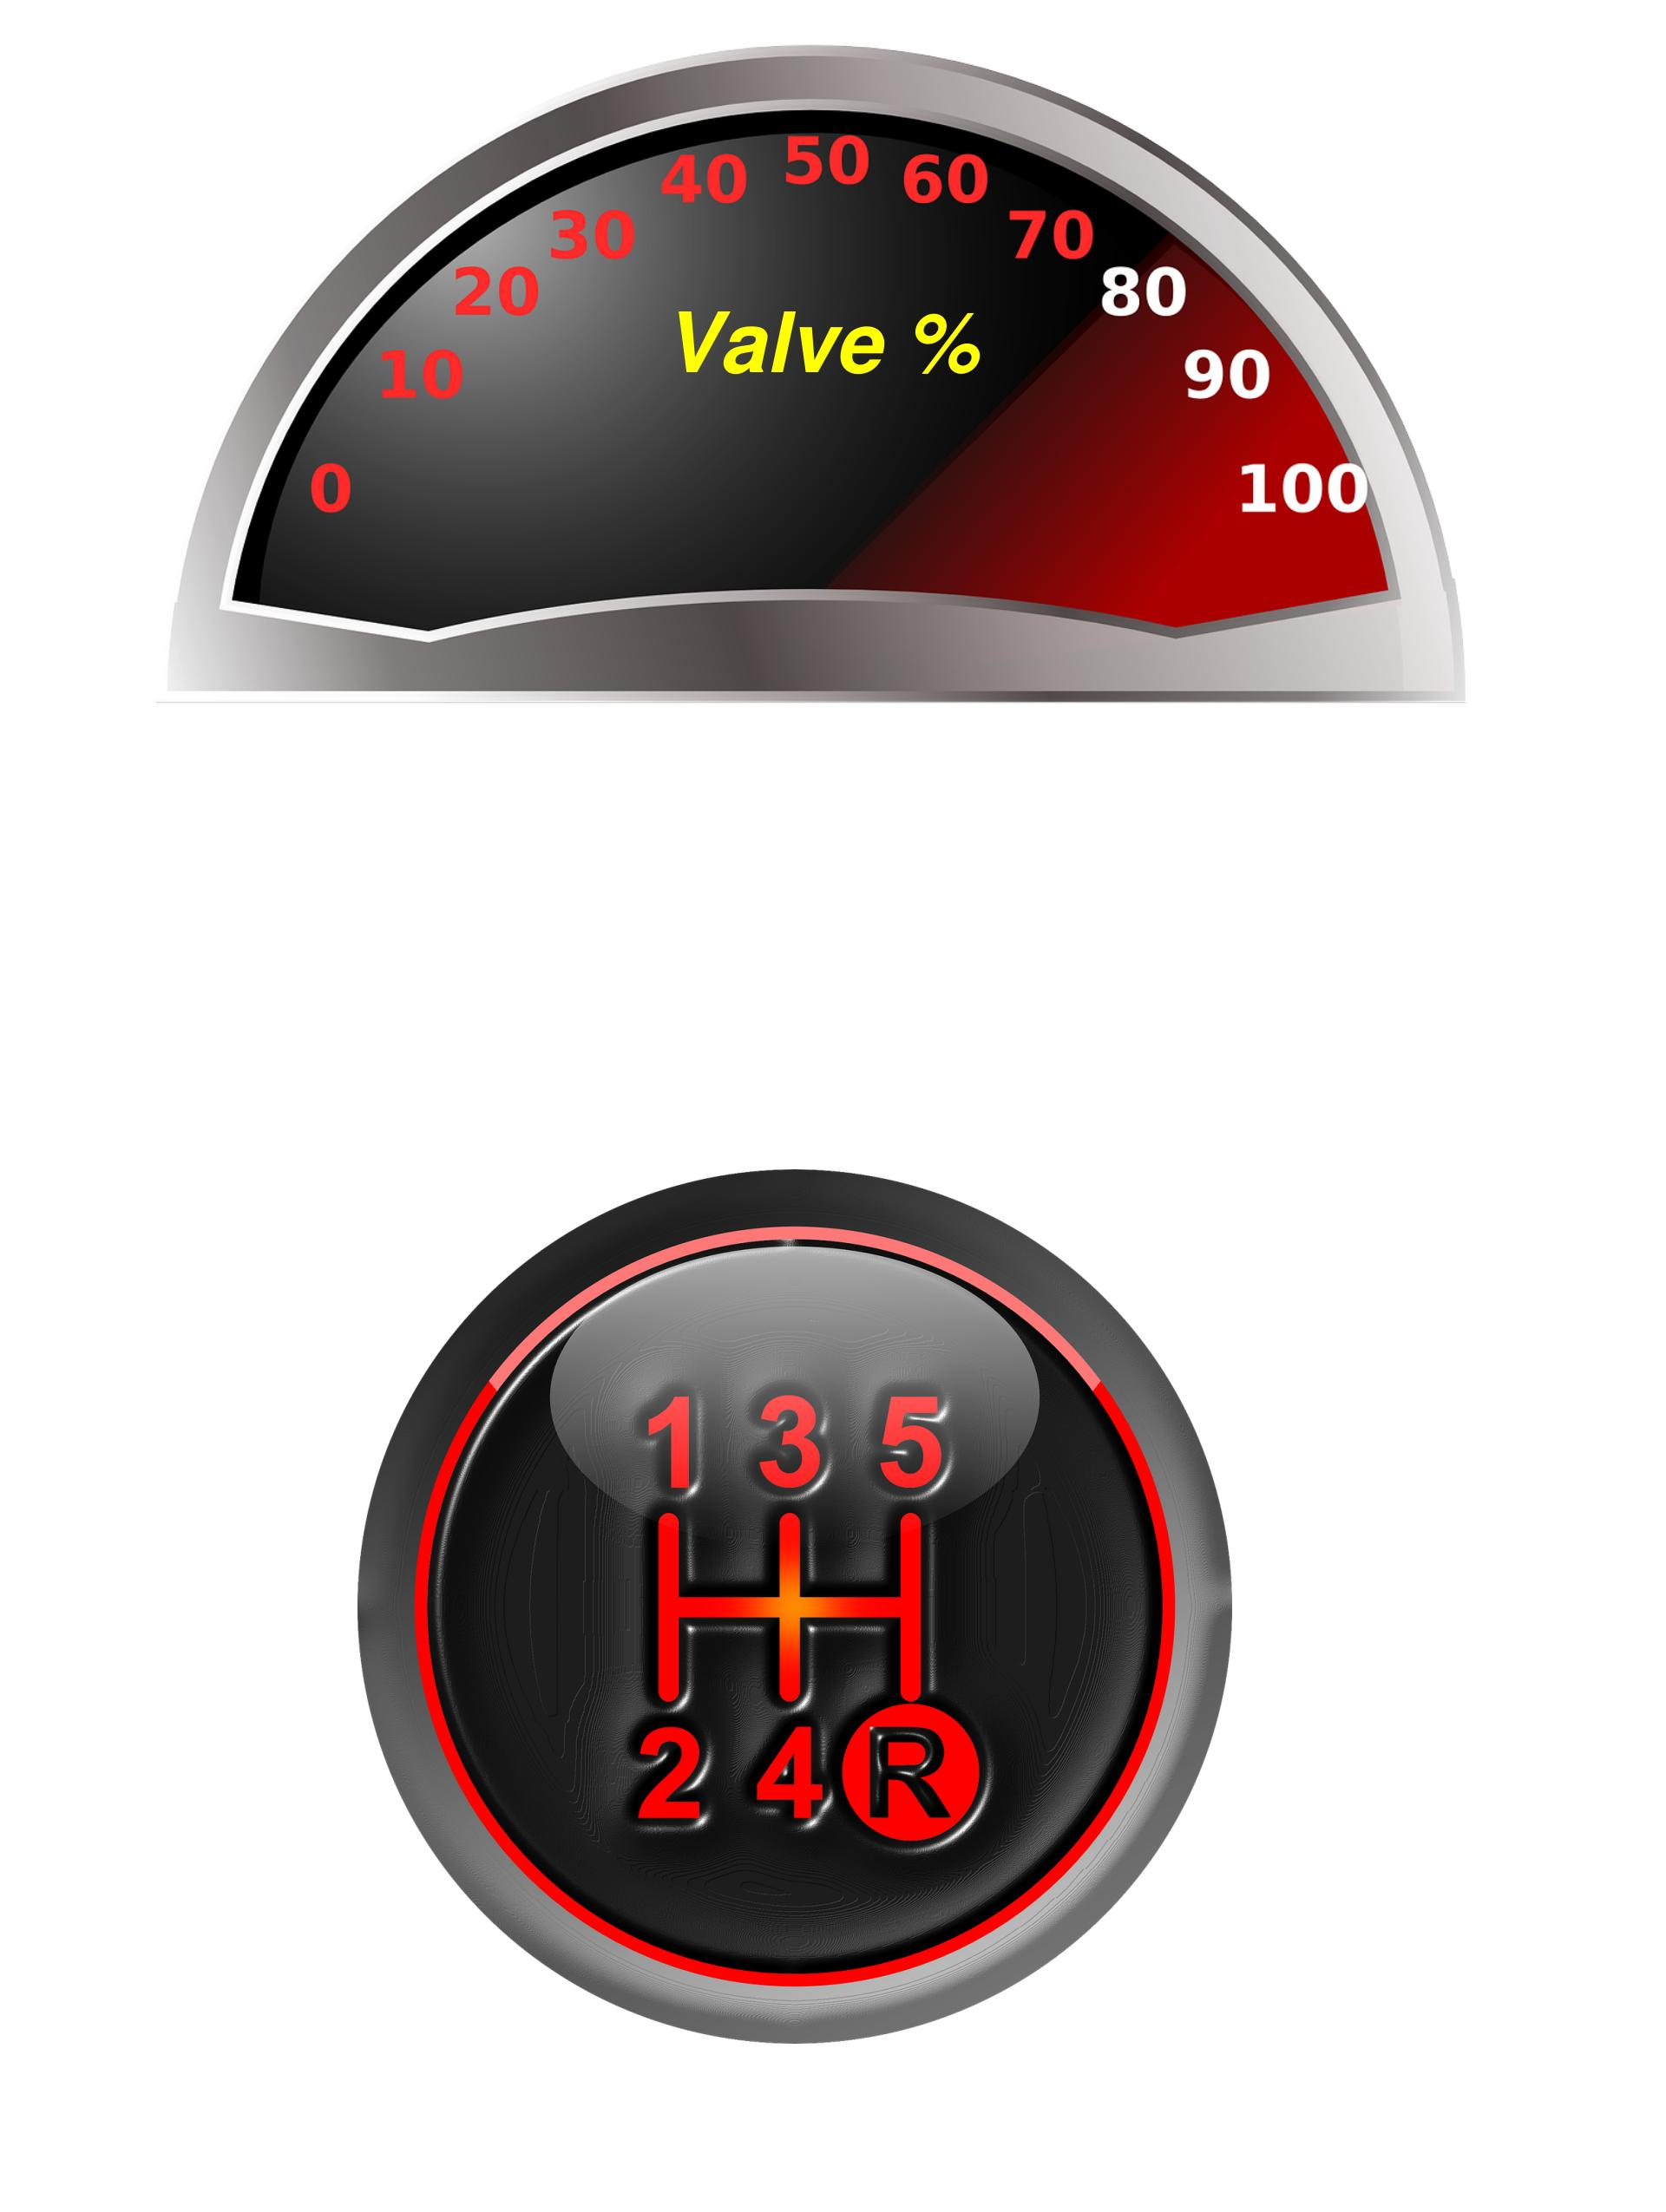
\includegraphics[height=6cm]{./Unit-01/img/Taxonomy-MvsL-2_cc0.jpg}}%
  \column[T]{0.70\textwidth}
   \begin{itemize}[<+-| alert@+>]
   \item Numeric, possibly quantised $\Rightarrow$ \TC{modulating} control\\
         (e.g., valve opening from 0 to 100\%,\\
         motor supply voltage from 0 to 24V in 0.1V steps,...);
         NOTE: \underline{any} such action has lower/upper bounds\\
         owing to physics.
   \item \vspace{10mm}Lexical ($\sim$bool/enum) $\Rightarrow$ \TC{logic} control\\
         (e.g., heater on/off,\\
          gear=\{reverse,neutral,1..5\},\\
          motor dir= \{forward,stop,backward\},...).
   \end{itemize}
 \end{columns}
\end{frame}

\begin{frame}[fragile]
\frametitleTC{Summarising}
\framesubtitleTC{brutally indeed}
\myPause
 \begin{itemize}[<+-| alert@+>]
 \item Controller:\\
         \begin{verbatim}
 type                     = {modulating,logic}
 timing                   = {continuous,discrete,event_triggered}
 connection_with_system   = {open-loop,closed_loop}
 disturbance_compensation = {present,absent}
         \end{verbatim}
 \item \vspace{-5mm}There are corner cases to this taxonomy, but for our purpose we can safely\\
       neglect them.
 \item In complex systems, controllers of different nature co-exist.
 \item \vfill To design and assess a controller, we need a modelling formalism.
 \item To make problems tractable, this formalism must also fit\\
       the controlled system.
 \item We thus move to the concept of \TC{dynamic system}.
 \end{itemize}
\end{frame}


\section{Dynamic systems}
\subsection{}

\begin{frame}\mccz
\frametitleTC{Foreword}
\framesubtitleTC{on how we shall proceed given the breadth of the subject}
\myPause
 \begin{columns}
  \column[T]{0.35\textwidth}
   \only<2 | handout:0>{\centering
\includegraphics[height=6cm]{./Unit-01/img/DynSys-Variety-1_cc0.jpg}}%
   \only<3 | handout:0>{\centering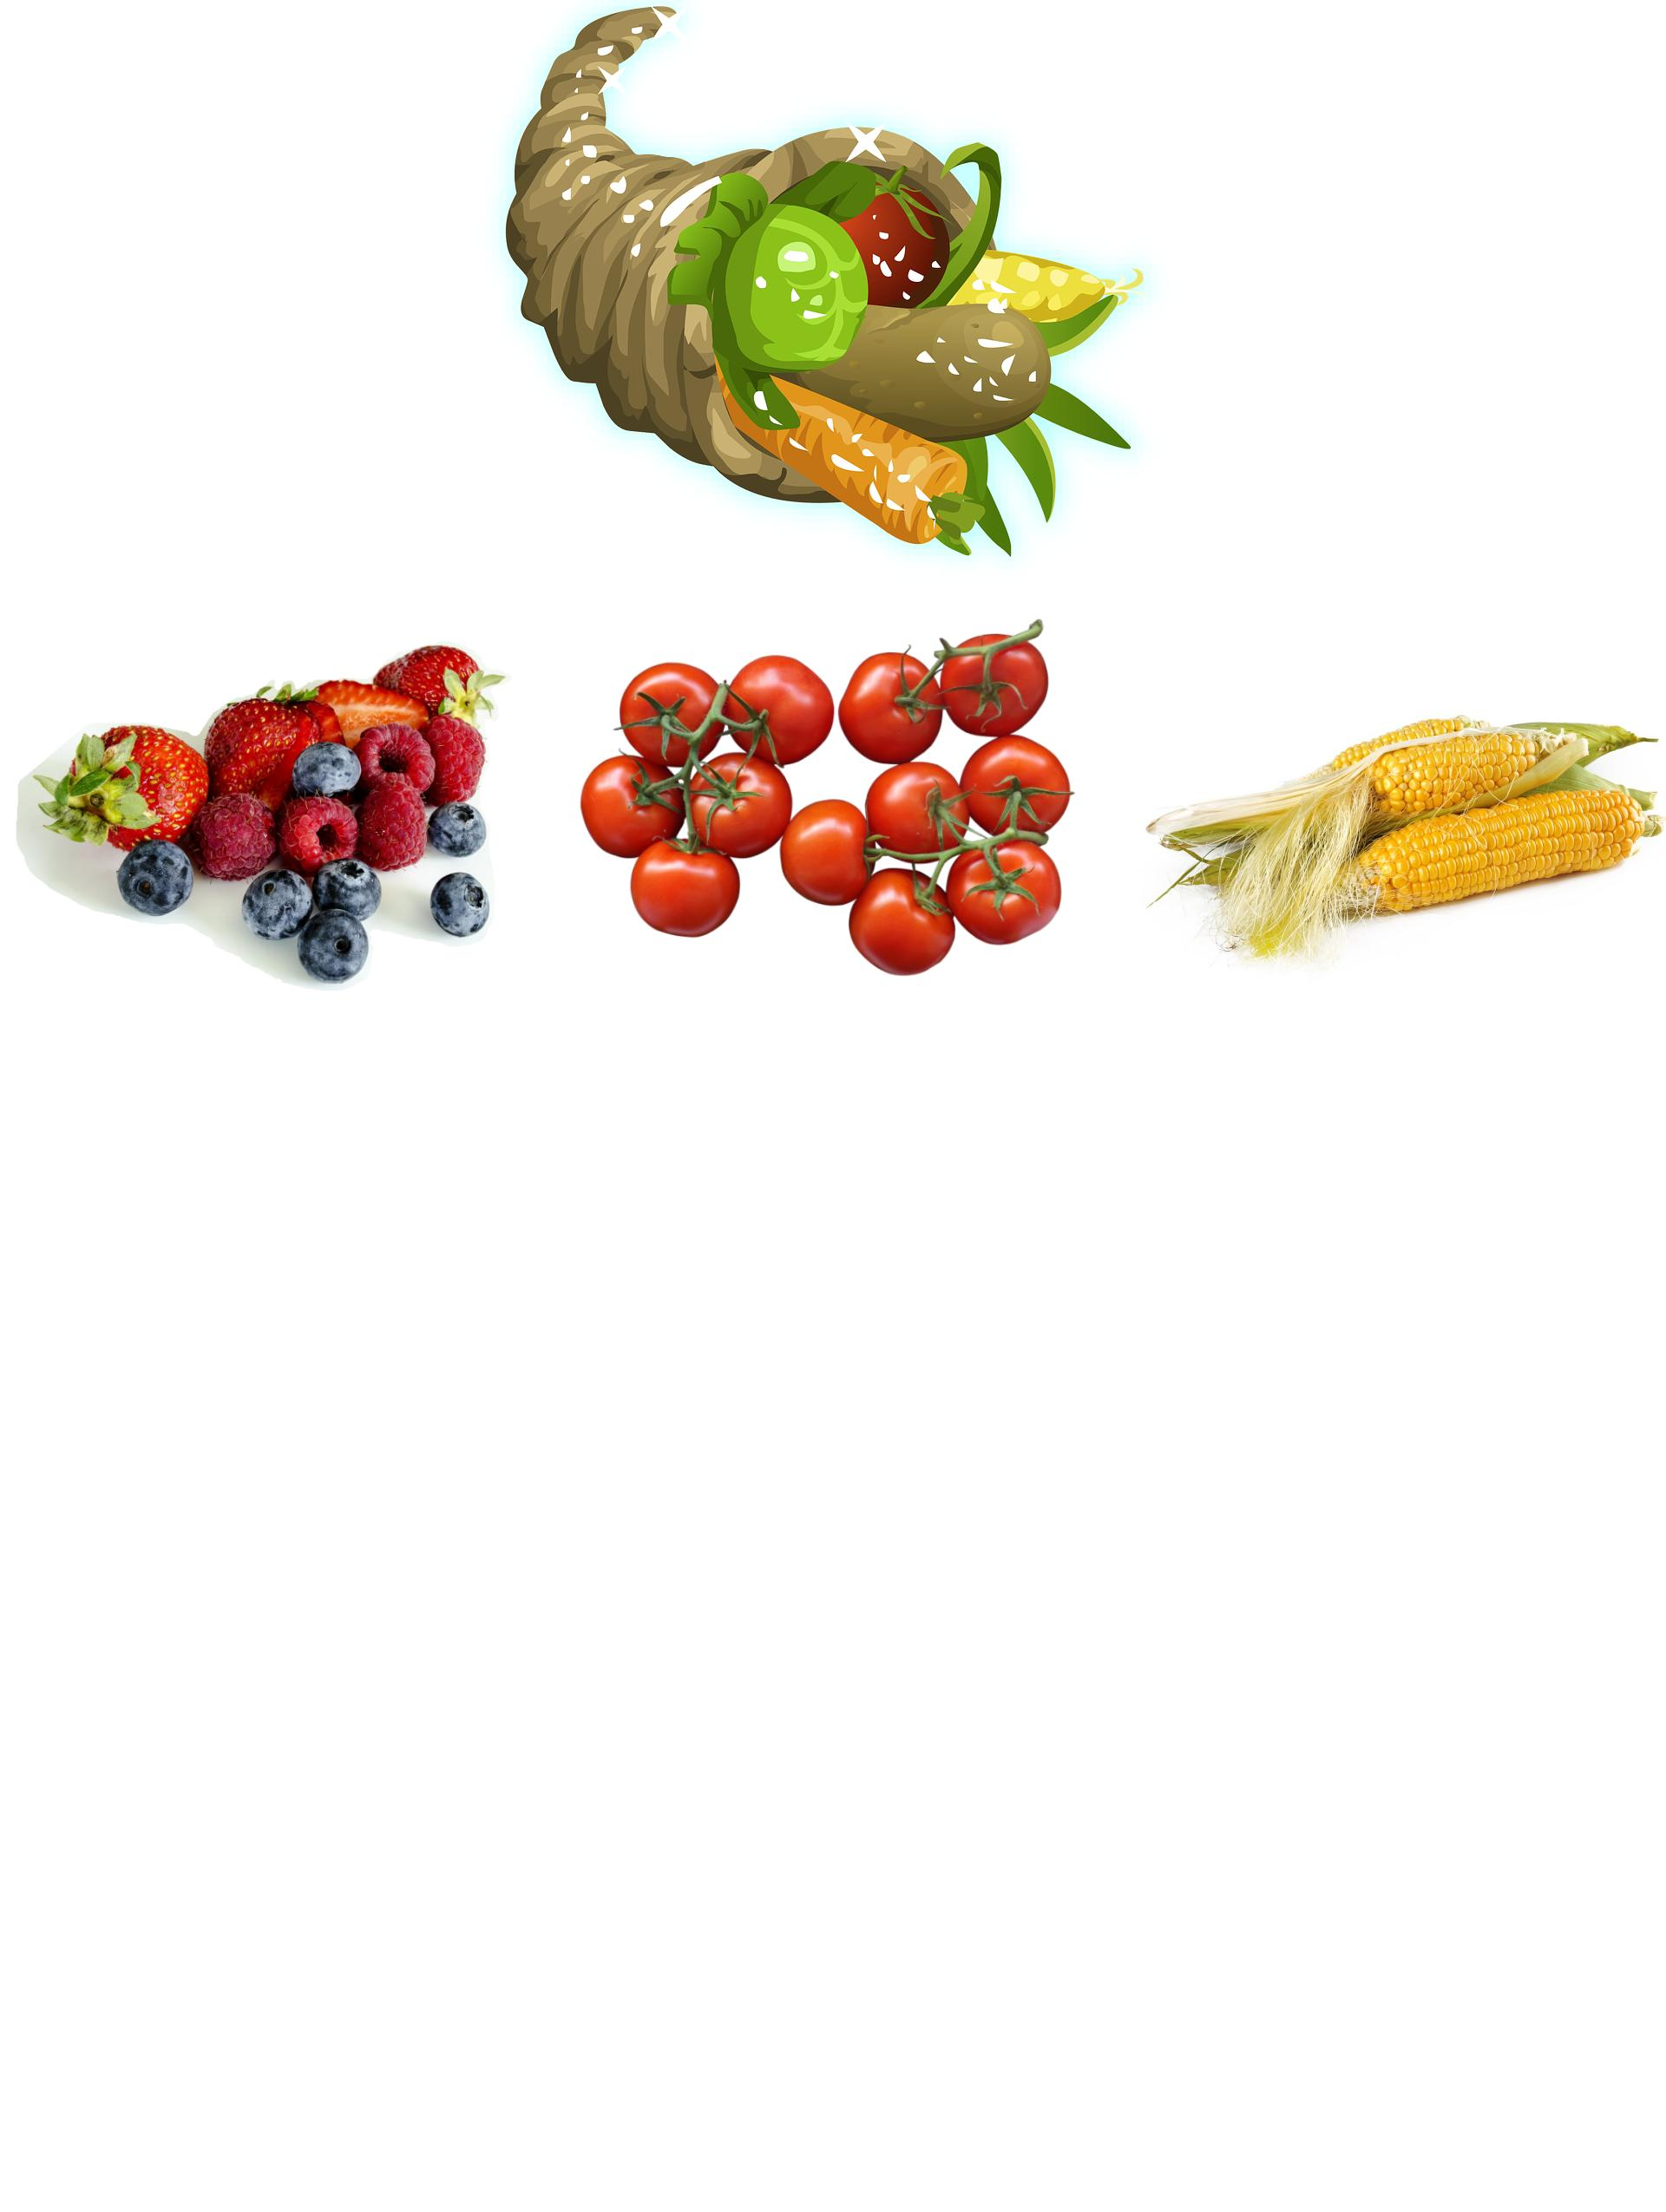
\includegraphics[height=6cm]{./Unit-01/img/DynSys-Variety-2_cc0.jpg}}%
   \only<4 | handout:0>{\centering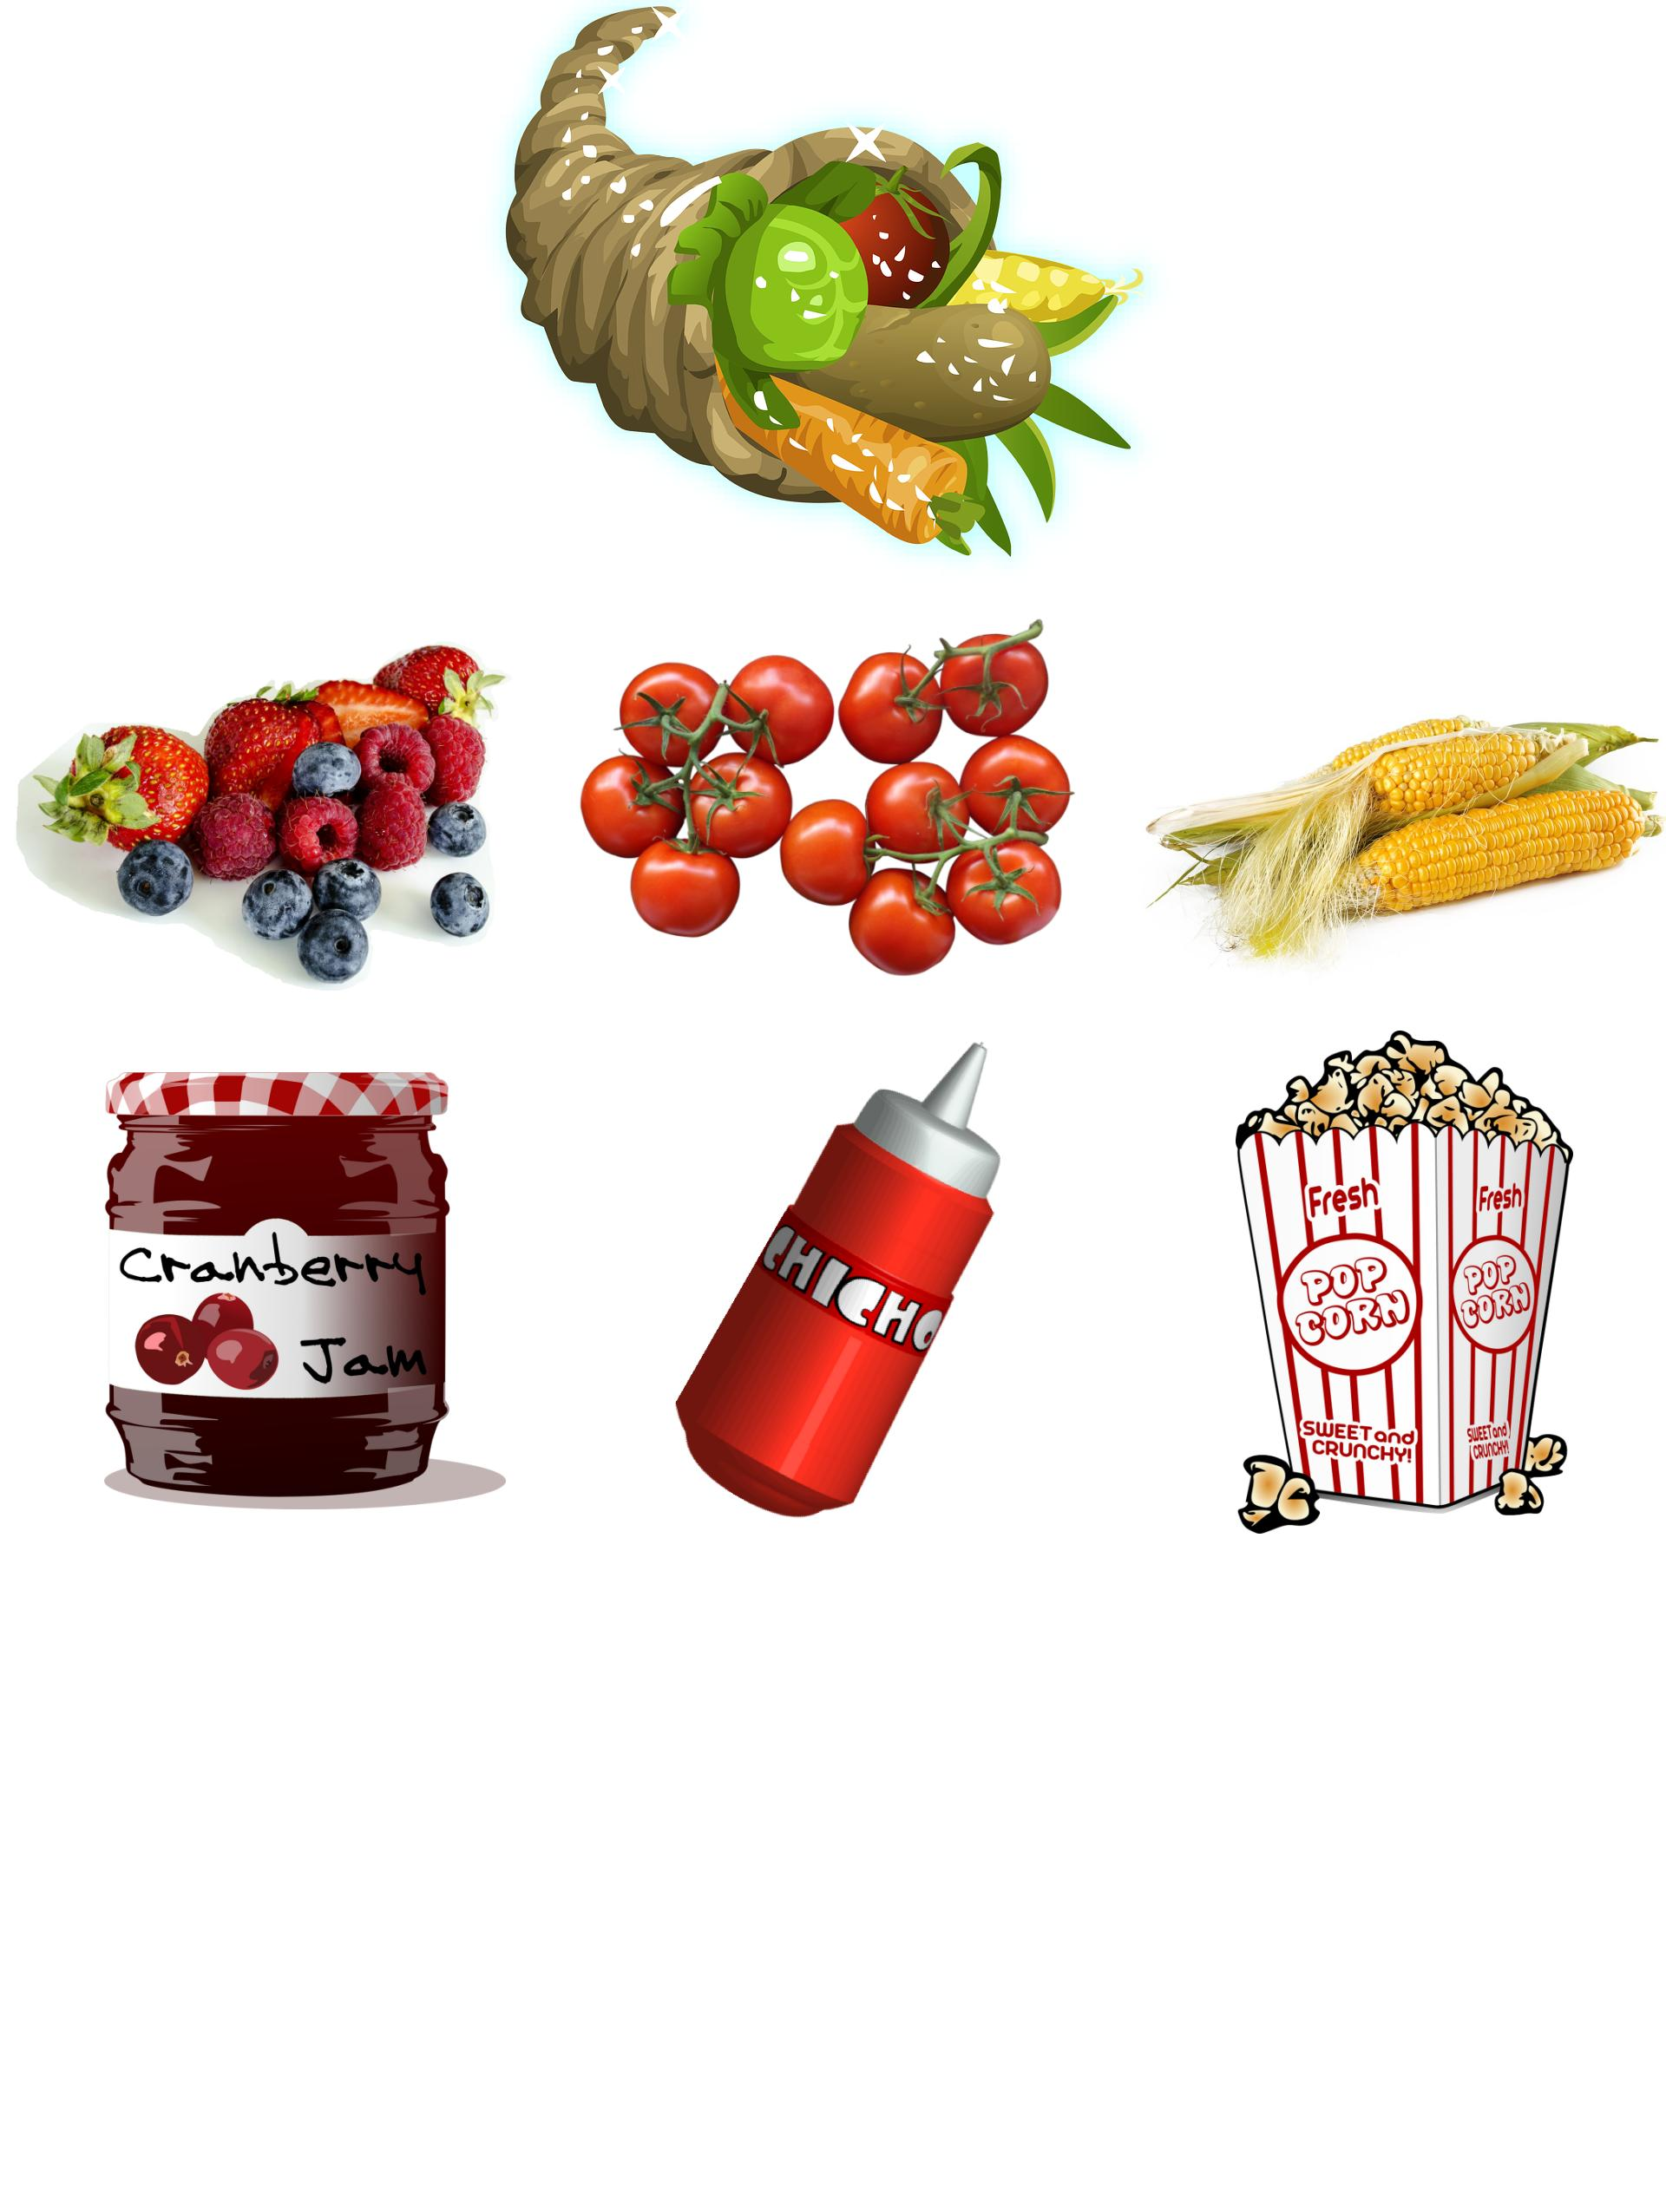
\includegraphics[height=6cm]{./Unit-01/img/DynSys-Variety-3_cc0.jpg}}%
   \only<5-           >{\centering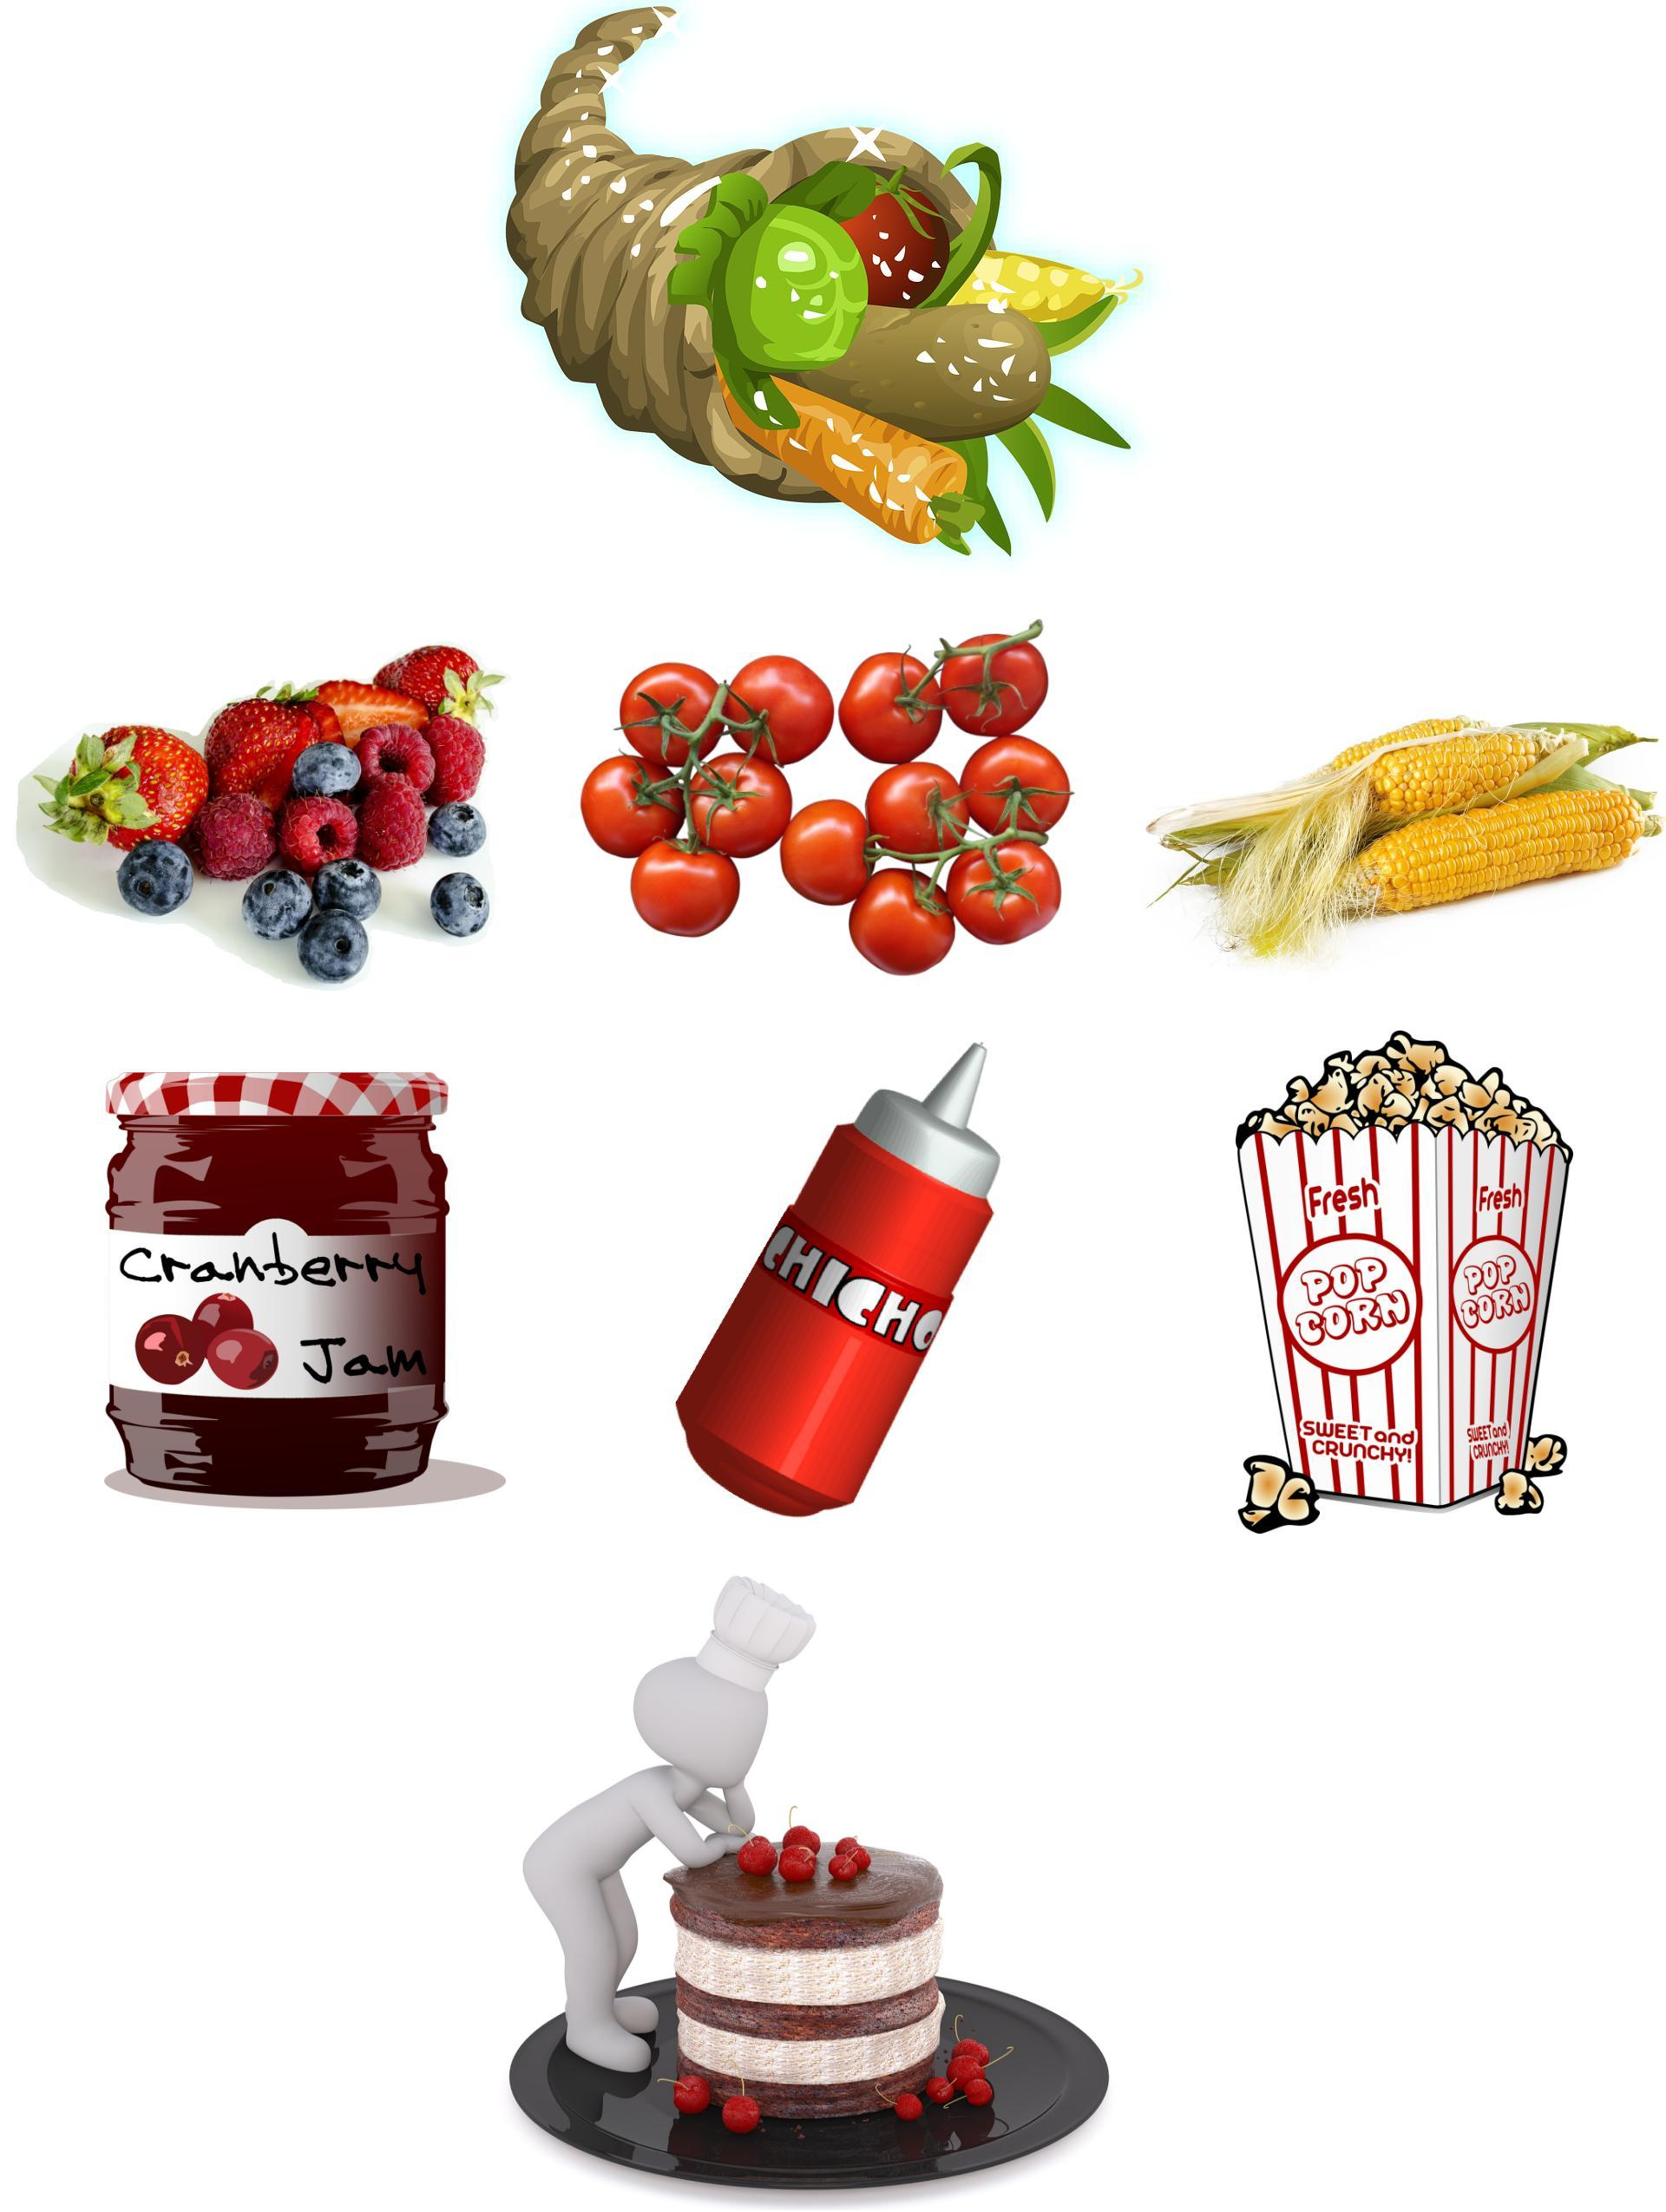
\includegraphics[height=6cm]{./Unit-01/img/DynSys-Variety-4_cc0.jpg}}%
  \column[T]{0.65\textwidth}
   \begin{itemize}[<+-| alert@+>]
   \item We shall state the \underline{general idea} of dynamic system,
   \item \vspace{8mm}then specialise to a few types of interest,
   \item \vspace{8mm}then see what control problems they fit,
   \item \vspace{8mm}and finally restrict to one type\\
         for the purpose of our activity.
   \end{itemize}
 \end{columns}
\end{frame}

\begin{frame}
\frametitleTC{Dynamic system}
\framesubtitleTC{General definition}
\myPause
 \begin{center}
  
\includegraphics[width=0.6\columnwidth]{./Unit-01/img/DynSys-GenericSystem.pdf}
  \myPause
 \end{center}
 \begin{itemize}[<+-| alert@+>]
 \item Suppose you know the values that the inputs have NOW.
 \item Can you tell which is NOW the values of the outputs?
 \item \vfill If so, the system is \TC{non dynamic}, otherwise it is \TC{dynamic.}
 \item Let us see some examples.
 \end{itemize}
\end{frame}

\begin{frame}
\frametitleTC{Dynamic system}
\framesubtitleTC{Introductory examples (1/3)}
\myPause
 \begin{itemize}[<+-| alert@+>]
 \item \textbf{Example 1}
       \begin{itemize}[<+-| alert@+>]
       \item[] \begin{tabular}{lll}
                System  &: & resistor of resistance $R$.\\
                Input   &: & applied voltage $V(t)$.\\
                Output  &: & flowing current $I(t)$.
               \end{tabular}
       \item \vspace{1mm}At time $\overline{t}$ the input is $V(\overline{t})=\overline{V}$; can you tell what
             the output $I(\overline{t})$ is?
       \item Yes, we have $I(\overline{t})=\overline{V}/R$.
       \item[] $\Rightarrow$ This system is non dynamic. 
       \end{itemize}
 \item \vfill\textbf{Example 2}
       \begin{itemize}[<+-| alert@+>]
       \item[] \begin{tabular}{lll}
                System  &: & water tank with inlet pump and outlet valve at the bottom.\\
                Inputs  &: & pump flowrate, valve opening.\\
                Output  &: & outlet flowrate.
               \end{tabular}
       \item \vspace{1mm}At time $\overline{t}$ we know the inlet pump flowrate and the outlet valve \\
             opening; can you tell what the output (outlet flowrate) is?
       \item No (it depends on valve opening and bottom pressure, i.e., level).
       \item[] $\Rightarrow$ This system is dynamic. 
       \end{itemize}
 \end{itemize}
\end{frame}

\begin{frame}
\frametitleTC{Dynamic system}
\framesubtitleTC{Introductory examples (2/3)}
\myPause
 \begin{itemize}[<+-| alert@+>]
 \item \textbf{Example 3}
       \begin{itemize}[<+-| alert@+>]
       \item[] \begin{tabular}{lll}
                System  &: & bus.\\
                Input   &: & $\Delta p(k)$, passengers on minus passengers off at stop $k$.\\
                Output  &: & passengers aboard when leaving stop $k$.
               \end{tabular}
       \item \vspace{1mm}At stop $k$ three passengers get on and two off, hence $\Delta p(k)=1$; can you tell\\
             how many passengers are aboard when leaving stop $k$?
       \item No (I should know how many were aboard before arriving at stop $k$).
       \item[] $\Rightarrow$ This system is dynamic. 
       \end{itemize}
 \end{itemize}
\end{frame}

\begin{frame}
\frametitleTC{Dynamic system}
\framesubtitleTC{Introductory examples (3/3)}
\myPause
 \begin{itemize}[<+-| alert@+>]
 \item \textbf{Example 4} -- note the slight difference
       \begin{itemize}[<+-| alert@+>]
       \item[] \begin{tabular}{lll}
                System  &: & lamp.\\
                Input   &: & button, when pressed the lamp goes on if off and \emph{vice versa}.\\
                Output  &: & lamp status (on/off).
               \end{tabular}
       \item \vspace{1mm}In the last hour we pressed the button 8 times;\\
             can you tell the status of the lamp?
       \item No (I should know the status 1 hour ago, however I can say that now\\
             the status is the same it was 1 hour ago).
       \item[] $\Rightarrow$ This system is dynamic. 
       \end{itemize}
 \end{itemize}
\end{frame}

\begin{frame}
\frametitleTC{Dynamic system}
\framesubtitleTC{Introductory examples -- summary for the dynamic cases}
\myPause
 \begin{itemize}[<+-| alert@+>]
 \item Example 2:
       \begin{itemize}[<+-| alert@+>]
       \item the system evolves in the continuous time,
       \item need to know the present tank level.
       \end{itemize}
 \item Example 3:
       \begin{itemize}[<+-| alert@+>]
       \item the system evolves in steps (stops 1 to last),
       \item need to know the previous bus occupancy.
       \end{itemize}
 \item Example 4:
       \begin{itemize}[<+-| alert@+>]
       \item the system evolves when events occur (no \emph{a priori} idea how many\\
             in a given timespan),
       \item need to know the initial lamp status.
       \end{itemize}
 \item \vfill So in general, to know the outputs, I need to know the inputs\\
       plus the present (or initial, or ``previous'' when applicable)\\
       value of something else.
 \item This "something else" is the system \TC{state.}
 \end{itemize}
\end{frame}

\begin{frame}
\frametitleTC{Classes of dynamic systems}
\framesubtitleTC{No theory, just intuition and abstraction from the examples}
\myPause
 \begin{itemize}[<+-| alert@+>]
 \item Common elements: input, output and \TC{state} (variables).
 \item Two equivalent viewpoints:
       \begin{itemize}[<+-| alert@+>]
       \item \underline{present state} and possibly present input $\Rightarrow$ present output\\
             (in the tank, opening and level now $\Rightarrow$ outlet flow now);
       \item \underline{initial state} and input story $\Rightarrow$ state and output story\\
             (initial level, inflow and opening story $\Rightarrow$ level and outflow story).
       \end{itemize}
 \item \vspace{2mm}General fact: dynamic systems
       \begin{itemize}[<+-| alert@+>]
       \item have memory of the past,
       \item and can respond differently to the same input, because they have a state.
       \end{itemize}
 \item \vfill Revisiting the examples and generalising, we shall now introduce\\
       three classes of dynamic systems:
       \begin{itemize}[<+-| alert@+>]
       \item continuous-time,
       \item discrete-time,
       \item and discrete-events.
       \end{itemize}
 \end{itemize}
\end{frame}

\begin{frame}
\frametitleTC{Continuous-time (CT) dynamic systems}
\myPause
 \begin{itemize}[<+-| alert@+>]
 \item They are made of \TC{differential equations.} Let us see what happens with the tank.
 \item Cylindrical tank of area $A$, fluid of constant density $\rho$, variable level $\ell(t)$
 \item Contained mass $M(t) = \rho A \ell(t)$.
 \item Bottom pressure $p(t) = \rho g \ell(t)$, where $g$ is gravity acceleration.
 \item Derivative of mass with time = inlet flowrate minus outlet flowrate.
 \item Inlet flowrate $w_i(t)$ is an input.
 \item Outlet flowrate $w_o(t)=A_v o(t) \sqrt{\rho p(t)}$, $A_v$ is a valve constant and $o(t)$ the opening.
 \item Valve opening $o(t)$ is an input, while $w_o(t)$ is the system output.
 \item The state is $\ell(t)$ and evolves from the initial value $\ell_0$ at $t=t_0$\\
       according to
       \begin{displaymath}
        \frac{dM(t)}{dt} = \rho A \frac{d\ell(t)}{dt} = w_i(t) - A_v o(t) \sqrt{\rho p(t)}, \quad
        \ell(t_0) = \ell_0.
       \end{displaymath}
 \end{itemize}
\end{frame}

\begin{frame}
\frametitleTC{Continuous-time dynamic systems}
\framesubtitleTC{In general}
\myPause
 \begin{itemize}[<+-| alert@+>]
 \item Input $u(t)$, state $x(t)$ with initial value $x_0$ at $t=t_0$, output $y(t)$;
       \begin{displaymath}
        \left\{\begin{array}{rll}
         \frac{dx(t)}{dt} &= f\left(x(t),u(t),t\right) &\quad \text{[State equation]} \\
         y(t)             &= g\left(x(t),u(t),t\right) &\quad \text{[Output equation]}
        \end{array}\right. \qquad
        x(t_0) = x_0.
       \end{displaymath}
 \item In the following for compactness we shall write $\dot{x}(t)$ to indicate $\frac{dx(t)}{dt}$.
 \item \vfill Enough on these systems for the moment (and for the great\\
       majority of our activity).
 \end{itemize}
\end{frame}

\begin{frame}
\frametitleTC{Discrete-time (DT) dynamic systems}
\myPause
 \begin{itemize}[<+-| alert@+>]
 \item They are made of \TC{difference equations.} Let us see what happens with the bus.
 \item Passengers after leaving stop $k$ = passengers before arriving at stop $k$ plus passengers on
       minus passengers off at stop $k$.
 \item Denote by $p(k)$ the passengers \underline{after} stop $k$ and by $\Delta p(k)$ the net variation
       or passengers (on minus off) at stop $k$, and we have
       \begin{displaymath}
        p(k) = p(k-1)+\Delta p(k).
       \end{displaymath}
 \end{itemize}
\end{frame}

\begin{frame}
\frametitleTC{Discrete-time dynamic systems}
\framesubtitleTC{In general}
\myPause
 \begin{itemize}[<+-| alert@+>]
 \item The integer $k$ is the ``time index'': it can really be time-related if it corresponds to the elapsing
       of a fixed period (giving rise to \TC{sampled-data} systems) or just count the evolution steps (bus stops,...).
 \item Input $u(t)$k, state $x(k)$ with initial value $x_0$ at $k=k_0$, output $y(k)$;
       \begin{displaymath}
        \left\{\begin{array}{rll}
         x(k) &= f\left(x(k-1),u(k-1),k\right) &\quad \text{[State equation]} \\
         y(k) &= g\left(x(k-1),u(k-1),k\right) &\quad \text{[Output equation]}
        \end{array}\right. \qquad
        x(k_0) = x_0.
       \end{displaymath}
 \item Read: at each step
       \begin{itemize}[<+-| alert@+>]
       \item I take the old state an the old input, and compute the new state,
       \item then I take the new state and the new input, and compute\\
             the new output.
       \end{itemize}
 \end{itemize}
\end{frame}

\begin{frame}
\frametitleTC{LTI (Linear, Time-Invariant) dynamic systems -- both CT and DT}
\framesubtitleTC{A specific but extremely useful subclass}
\myPause
 \begin{itemize}[<+-| alert@+>]
 \item \vspace{2mm}Linear: functions $f(\cdot,\cdot,\cdot)$ and  $g(\cdot,\cdot,\cdot)$ linear in $x$ and $u$.
 \item Time-invariant: $f$ and $g$ do not depend explicitly on $t$ (CT case) or $k$ (DT case).
 \item Input $u(t|k)$, state $x(t|k)$ with initial value $x_0$ at $t|k=t_0|k_0$, output $y(t|k)$;
       \begin{displaymath}
         \begin{array}{lll}
          \text{CT case:} & 
          \left\{\begin{array}{rll}
           \dot{x}(t) &= Ax(t)+bu(t) \\
           y(t)       &= cx(t)+du(t)
          \end{array}\right. &
          x(0) = x_0 \\ \\
          \text{DT case:} & 
          \left\{\begin{array}{rll}
           x(k) &= Ax(k-1)+bu(k-1) \\
           y(k) &= cx(k)+du(k)
          \end{array}\right. &
          x(0) = x_0
         \end{array}
        \end{displaymath}
 \item \vfill The time origin is zero because the system is time-invariant (TI).
 \item $A$, $b$, $c$ and $d$ are matrices of convenient dimensions. 
 \end{itemize}
\end{frame}

\begin{frame}
\frametitleTC{Discrete-event dynamic systems}
\myPause
 \begin{itemize}[<+-| alert@+>]
 \item Not driven by time but rather by events.
 \item Represented as automata, Petri nets, and the like.
 \item Example automaton for the lamp:
       \begin{center}
        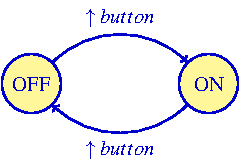
\includegraphics[width=0.30\columnwidth]{./Unit-01/img/DynSys-LampAutomaton.pdf}
       \end{center}
 \item In our activity we are not addressing this kind of systems.
 \item Let us move to a \emph{rough} (system class)--(control problem) pairing.
 \end{itemize}
\end{frame}

\begin{frame}
\frametitleTC{Dynamic systems classes and control problems}
\framesubtitleTC{...this time looking at computers -- just an overview to stimulate discussion}
\myPause
 \begin{itemize}[<+-| alert@+>]
 \item Group 1 -- problems directly related to physics \emph{stricto sensu}:
       \begin{itemize}[<+-| alert@+>]
       \item typical example -- CPU temperature;
       \item system model -- continuous-time dynamic system;
       \item controller design -- as continuous-time system, then converted to discrete-time\\
             to become control \TC{code}.
       \end{itemize}
 \item Group 2 -- problems not in group 1 where requirements are translatable into desired behaviours
       of signals (reference or admissible range):
       \begin{itemize}[<+-| alert@+>]
       \item typical example -- deadline enforcement, obtained by tracking a desired completion\\
             that reaches 100\% by the deadline (\underline{many} problems can be formulated\\
             this way or analogously);
       \item system model -- discrete-time dynamic system;
       \item controller design -- as discrete-time system, then code.
       \end{itemize}
 \item Group 3 -- anything else:
       \begin{itemize}[<+-| alert@+>]
       \item mixed design strategy (not in the scope of our activity),
       \item or not suited for a control-theoretical design.
       \end{itemize}
 \end{itemize}
\end{frame}


\section{Conclusions}
\subsection{}

\begin{frame}
\frametitleTC{Conclusions}
\framesubtitleTC{Recap and lessons learnt (1/3)}
\myPause
 \begin{itemize}[<+-| alert@+>]
 \item Control is \TC{governing a phenomenon} (physical or not).
 \item This means determining \TC{actions} on that phenomenon, based on \TC{requirements}\\
       and possibly \TC{measurements}.
 \item Major issues are exogenous actions -- or \TC{disturbances} -- and \TC{uncertainty},\\
       i.e., only partial knowledge of the controlled system.
 \item Quite often a control problem can be formulated in terms of signals,\\
       i.e., as \TC{tracking a reference} and/or \TC{rejecting disturbances}.
 \end{itemize}
\end{frame}

\begin{frame}
\frametitleTC{Conclusions}
\framesubtitleTC{Recap and lessons learnt (2/3)}
\myPause
 \begin{itemize}[<+-| alert@+>]
 \item A controller may or may not know the effects of its action on the controlled system, giving rise to
       \TC{closed-loop} (or \TC{feedback}) versus \TC{open-loop} control.
 \item A controller can operate in the continuous time, but in computing systems this is\\
       practically never the case;
 \item hence for us a controller is a piece of code, invoked either periodically or based\\
       on events, giving rise to \TC{discrete-time} versus \TC{event-based} control.
 \item Control signals can be \TC{numeric} or \TC{lexical}, corresponding to \TC{modulating}\\
       versus \TC{logic} control.
 \item Control problems are posed and treated with reference to one\\
       or more classes of \TC{dynamic systems}. 
 \end{itemize}
\end{frame}

\begin{frame}
\frametitleTC{Conclusions}
\framesubtitleTC{Recap and lessons learnt (3/3)}
\myPause
 \begin{itemize}[<+-| alert@+>]
 \item Dynamic systems have a \TC{state}, hence they
       \begin{itemize}[<+-| alert@+>]
       \item remember the past,
       \item or -- equivalently -- their initial condition,
       \item and thus \TC{can produce different outputs in response to the same input}...
       \item ...without however being time-varying or ``adaptive'' (remember this remark!).
       \end{itemize}
 \item We have seen some classes of dynamic systems.
 \item In the following we shall concentrate on LTI ones, almost exclusively\\
       in the DT domain. 
 \end{itemize}
\end{frame}

\section{}
{
\setbeamertemplate{headline}{
  \begin{beamercolorbox}[wd=\paperwidth,ht=4.2ex,dp=1.5ex]{palette quaternary}
  \end{beamercolorbox}
  }
\setbeamertemplate{footline}{
  \begin{beamercolorbox}[wd=\paperwidth,ht=2.2ex,dp=1.5ex]{palette quaternary}
  \end{beamercolorbox}
  }
\begin{frame}[noframenumbering]
 \vspace{20mm}\Huge{Discussion open}
\end{frame}
}








%%% UNIT 2
{
\setbeamertemplate{headline}{}
\setbeamertemplate{footline}{
  \begin{beamercolorbox}[wd=\paperwidth,ht=2.2ex,dp=1.5ex]{palette quaternary}
  \end{beamercolorbox}
  }
\begin{frame}[noframenumbering]
\frametitle{\DB{\huge{\textbf{$\blacksquare$ Unit 2}}}}
\myPause
 \begin{itemize}
 \item[] \LARGE{\MB{Feedback and its magic}}
 \item[] \vspace{-1mm}\LARGE{\MB{Dynamic systems}}
 \item[] \vspace{-1mm}\LARGE{\MB{The DT LTI case in detail}}
 \item[] \vspace{-1mm}\LARGE{\MB{Conclusions and discussion}}
 \end{itemize}
\end{frame}
}

\part{}

\section{Feedback (informally)}
\subsection{}

\begin{frame}\mccz
\frametitleTC{Feedback and its magic}
\myPause
 \begin{columns}
  \column[T]{0.45\textwidth}
   \only<2->{\centering
\includegraphics[height=6cm]{./Unit-02/img/Feedback-TheMagic_cc0.jpg}}\myPause%
  \column[T]{0.55\textwidth}
   \begin{itemize}[<+-| alert@+>]
   \item If PROPERLY used, feedback can
         \begin{itemize}[<+-| alert@+>]
         \item \vspace{2mm}counteract model errors\\
                and uncertainties,
         \item \vspace{2mm}reject a disturbance\\
                without the need\\
                for its measurement,
         \item \vspace{2mm}stabilise an unstable\\
               or ``runaway'' system.
         \end{itemize}
   \item \vspace{4mm}Let us see.
   \end{itemize}
 \end{columns}
\end{frame}

\begin{frame}
\frametitleTC{Feedback to counteract model errors/uncertainty and disturbances}
\framesubtitleTC{(to introduce this idea we do not use dynamic systems for simplicity)}
\myPause
 \begin{itemize}[<+-| alert@+>]
 \item \vspace{-8mm}Consider a controlled system such that the outcome $O$ depends on the control action $A$ and
       the disturbance $D$ as \textcolor{magenta}{$O=0.5(A+D)$.}
 \item If we want to use open-loop control and to make $O$ equal a reference $R$, we must solve for $A$ the equation
       $0.5(A+D)=R$, whence the control law \DG{$A=2R-D$.}
 \item Let us verify with some numbers:
 \item[] \begin{center}
          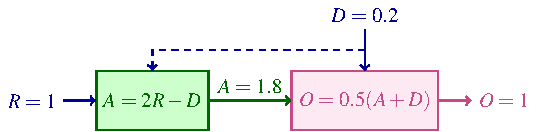
\includegraphics[width=0.60\columnwidth]{./Unit-02/img/Taxonomy-OpenLoop-Example-FullKnowledge.pdf}
          \hspace{6mm}
\includegraphics[height=1.5cm]{./Unit-02/img/smile.png}
         \end{center}
 \end{itemize}
\end{frame}

\begin{frame}
\frametitleTC{Feedback to counteract model errors/uncertainty and disturbances}
\myPause
 \begin{itemize}[<+-| alert@+>]
 \item But what if we assume \textcolor{magenta}{$O=0.5(A+D)$} while the true system is
       \textcolor{magenta}{ $O=\mathbf{0.6}(A+D)$}?
 \item If we use the nominal control law \DG{$A=2D-R$} on the true system, we get the following:
 \item[] \begin{center}
          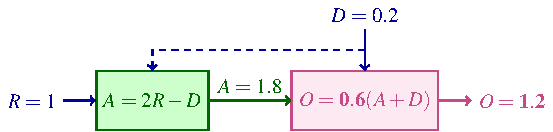
\includegraphics[width=0.65\columnwidth]{./Unit-02/img/Taxonomy-OpenLoop-Example-PartialKnowledge.pdf}
          \hspace{6mm}
\includegraphics[height=1.5cm]{./Unit-02/img/frown.png}
         \end{center}
 \item \vfill H\'{e}las, 20\% error on a model parameter (0.6 instead of 0.5)\\
       $\Rightarrow$ 20\% error of $O$ wrt $R$.
 \item Open-loop control cannot counteract model errors.
 \item Let us try with feedback.
 \end{itemize}
\end{frame}

\begin{frame}
\frametitleTC{Feedback to counteract model errors/uncertainty and disturbances}
\myPause
 \begin{itemize}[<+-| alert@+>]
 \item \underline{EXAMPLE} feedback scheme with \TC{proportional} control (action $A$ proportional\\
       to the \TC{error} $R-O$); note that we do not compensate the disturbance:
 \item[] \begin{center}
          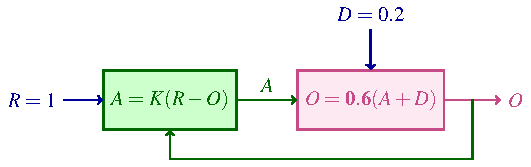
\includegraphics[width=0.60\columnwidth]{./Unit-02/img/Taxonomy-ClosedLoop-Example.pdf}
         \end{center}
 \item Joining the system and controller equations, for $O$ we get
       \begin{displaymath}
        \begin{array}{rcl}
         \left\{\begin{array}{rl}
          A &= K(R-O) \\
          O &= 0.6(A+D)
         \end{array}\right. &
         \Rightarrow &
          O = \frac{3K}{3K+5}R+\frac{3}{3K+5}D
         \end{array}
        \end{displaymath}
 \item Apparently, as $K \rightarrow \infty$, $O \rightarrow R$ $\forall D$.
 \item \vfill Yes, feedback can counteract model errors and disturbances;
 \item possible drawbacks on stability (improper use of feedback) later on. 
 \end{itemize}
\end{frame}

\begin{frame}
\frametitleTC{Studying the stability of a system}
\framesubtitleTC{adopting here a \underline{very} informal attitude, where ``stable'' means ``left alone, does not
                 run amok''}
\myPause
 \begin{itemize}[<+-| alert@+>]
 \item Let us take our system, initialise $y(0)$ to $y_0$, let $u(k)=0$ $\forall k$ so that
       \begin{displaymath}
        y(k) = ay(k-1),
       \end{displaymath}
       and see what happens.
 \item \vfill Case 1: $|a|<1$, for example 0.5 or -0.5.\\
 \item[] For $k=0,1,2,\ldots$, we have respectively the $y$ sequences
       \begin{displaymath}
        \begin{matrix*}[r]
          y_0, &  0.5y_0, & 0.25y_0, &  0.125y_0, \ldots \\
          y_0, & -0.5y_0, & 0.25y_0, & -0.125y_0, \ldots
        \end{matrix*}
       \end{displaymath}       
 \item[] For $k\rightarrow\infty$ the system's \TC{free motion} (no input) converges to zero\\
         $\Rightarrow$ we say the system is \TC{asymptotically stable.}      
 \end{itemize}
\end{frame}

\begin{frame}
\frametitleTC{Studying the stability of a system}
\myPause
 \begin{itemize}[<+-| alert@+>]
 \item Case 2: $|a|=1$, i.e., $a=\pm 1$.\\
 \item[] For $k=0,1,2,\ldots$, we have respectively the $y$ sequences
       \begin{displaymath}
        \begin{matrix*}[r]
          y_0, &  y_0, & y_0, &  y_0, \ldots \\
          y_0, & -y_0, & y_0, & -y_0, \ldots
        \end{matrix*}
       \end{displaymath}       
 \item[] For $k\rightarrow\infty$ the free motion neither converges to zero nor diverges\\
         $\Rightarrow$ we say the system is \TC{stable}, but not asymptotically.
 \item \vfill Case 3: $|a|>1$, for example 2 or -2.\\
 \item[] For $k=0,1,2,\ldots$, we have respectively the $y$ sequences
       \begin{displaymath}
        \begin{matrix*}[r]
          y_0, &  2y_0, & 4y_0, &  8y_0, \ldots \\
          y_0, & -2y_0, & 4y_0, & -8y_0, \ldots
        \end{matrix*}
       \end{displaymath}
 \item[] For $k\rightarrow\infty$ the free motion diverges (except for the one case $y_0=0$)\\
         $\Rightarrow$ we say the system is \TC{unstable.} 
 \end{itemize}
\end{frame}


\begin{frame}
\frametitleTC{Stabilising a system by means of feedback}
\myPause
 \begin{itemize}[<+-| alert@+>]
 \item Take an unstable system:
       \begin{displaymath}
        y(k) = ay(k-1)+u(k-1), \qquad a=2.
       \end{displaymath}
 \item Feed $y$ back to $u$ proportionally, i.e., set $u(k) = Qy(k)$.
 \item Doing so we have the closed-loop system
       \begin{displaymath}
        y(k) = 2y(k-1)+Qy(k-1) = (2+Q)y(k-1)
       \end{displaymath}
       and if we chose $Q$ so that $|2+Q|<1$, this is asymptotically stable.
 \end{itemize}
\end{frame}

\begin{frame}
\frametitleTC{Stabilising a system by means of feedback}
\framesubtitleTC{and once again, tolerating model errors/uncertainties}
\myPause
 \begin{itemize}[<+-| alert@+>]
 \item Note that feedback control is also naturally \TC{robust} (for the moment,\\
       think of this as ``resilient to model errors'').
 \item For example, take $Q=-1.5$ so that $2+Q=0.5$.
 \item In this case the closed loop is asymptotically stable not only for $a=2$,\\
       but $\forall a$ s.t. $|a+Q|=|a-1.5|<1$, i.e., for $0.5<a<2.5$.
 \item \vspace{4mm} Summing up, with feedback we can impose stability even if we do not know\\
       the system (here, parameter $a$) precisely...
 \item[]\vspace{-1mm} ...but for the very same reasons, we might also \emph{destroy} stability.
 \item Feedback is a powerful weapon, use with care.
 \item \vfill And now, let us re-address feedback and dynamic systems\\
       with a formal attitude (soon focusing on the DT LTI case).
 \end{itemize}
\end{frame}



\section{Dynamics (formally)}
\subsection{}

\begin{frame}
\frametitleTC{System -- recap and systematisation}
\framesubtitleTC{A mathematical representation (model) of something that evolves}
\myPause
 \begin{columns}
  \column[T]{0.45\textwidth}
   \begin{itemize}[<+-| alert@+>]
   \item[] Simple representation
   \item[] \vspace{2mm}\begin{center}
            \usetikzlibrary{matrix}
\usetikzlibrary{arrows}
\usetikzlibrary{calc}

\tikzstyle{block} = [draw,rectangle,thick,minimum height=3em,minimum width=4em]
\tikzstyle{sum} = [draw,circle,inner sep=0mm,minimum size=2mm]
\tikzstyle{connector} = [->,thick]

\begin{tikzpicture}[scale=1.00]

\node [left] at (00.00,00.00) (in_u) {$u$};
\node [block] at (01.20,00.00) (S) {{\huge$\mathcal{S}$}};
\draw [connector] (in_u.east) -- (S.west);
\node [right] at (02.40,00.00) (out_y) {$y$};
\draw [connector] (S.east) -- (out_y.west);
\end{tikzpicture}


           \end{center}
           \begin{itemize}[<+-| alert@+>]
           \item[] $u$ -- input(s)
           \item[] $y$ -- output(s)
           \end{itemize}
   \end{itemize}
  \column[T]{0.55\textwidth}
   \begin{itemize}[<+-| alert@+>]
   \item[] Model ingredients
           \begin{itemize}[<+-| alert@+>]
           \item what the system evolves upon:
                 \begin{itemize}[<+-| alert@+>]
                 \item the \TC{continuous time} $t$;
                 \item an integer index $k$ counting some events,
                       frequently called\\the \TC{discrete time}.
                 \end{itemize}
           \item the \TC{evolution law}:
                 \begin{itemize}[<+-| alert@+>]
                 \item $u[t_0,t]\;\rightarrow\;y[t_0,t]$;
                 \item $u[k_0,k]\;\rightarrow\;y[k_0,k]$.
                 \end{itemize}
           \end{itemize}
   \end{itemize}
 \end{columns} \myPause
 \vfill
 \begin{center}
  \vfill \textbf{Is anything missing? \myPause Sometimes, yes.}
 \end{center}
\end{frame}

\begin{frame}
\frametitleTC{\underline{Dynamic} system -- recap and systematisation}
\framesubtitleTC{The most general definition}
\myPause
\begin{center}
 {\Large
 If the knowledge of $u[t_0,t]$ --- or $u[k_0,k]$ \\ \myPause
 allows to determine $y[t_0,t]$ --- or $y[k_0,k]$ \\ \myPause
 the system is said to be \TC{non dynamic},\\ \myPause
 \vspace{1.5mm}\TC{dynamic} otherwise. \myPause
 }
\end{center}
\end{frame}

\begin{frame}
\frametitleTC{Dynamic system -- recap and systematisation}
\framesubtitleTC{Input, output, and \emph{state}}
\myPause
\begin{itemize}[<+-| alert@+>]
\item Non dynamic system:\\
      $y[t_0,t]$ or $y[k_0,k]$ depends only on $u[t_0,t]$ or $u[k_0,k]$.
\item Dynamic system:\\
      $y[t_0,t]$ or $y[k_0,k]$ depends on $u[t_0,t]$ or $u[k_0,k]$,\\
      and on the initial values $x[t_0]$ or $x[k_0]$ of some quantities.
\item These are called the \TC{state variables}, and form the \TC{state (vector)}.
\item The number of state variables is called the \TC{order} of the system.
\end{itemize}
\end{frame}

\begin{frame}
\frametitleTC{Dynamic system -- recap and systematisation}
\framesubtitleTC{How can we express this in mathematical terms?}
\myPause
In several ways. We see the only two relevant for us.\myPause
\begin{itemize}[<+-| alert@+>]
\item Continuous-Time (CT) system:\\
      \begin{displaymath}
       \left\{
        \begin{array}{rl}
         \frac{dx(t)}{dt} &= f \big( x(t),u(t),t  \big) \\
         y(t)             &= g \big( x(t),u(t),t  \big)
        \end{array}
       \right.
      \end{displaymath}
\item Discrete-Time (DT) system:\\
      \begin{displaymath}
       \left\{
        \begin{array}{rl}
         x(k) &= f \big( x(k-1),u(k-1),k  \big) \\
         y(k) &= g \big( x(k),u(k),k  \big)
        \end{array}
       \right.
      \end{displaymath}

\end{itemize}
\end{frame}

\begin{frame}
\frametitleTC{Dynamic system -- recap and systematisation}
\framesubtitleTC{Some more definitions (for both the CT and the DT case)}
\myPause
\begin{itemize}[<+-| alert@+>]
\item \TC{Linear (L)} system:\\
      $f(\cdot,\cdot,\cdot)$ and $g(\cdot,\cdot,\cdot)$ linear in $x$ and $u$.
\item \TC{Time-Invariant (TI)} system:\\
      $f(\cdot,\cdot,\cdot)$ and $g(\cdot,\cdot,\cdot)$ not depending on $t$ or $k$.
\item \TC{Proper} (sometimes, \emph{strictly} proper) system:\\
      $g(\cdot,\cdot,\cdot)$ not depending on $x$,\\
      i.e., the input acts on the output only through the state.
\item \TC{SISO} (Single-Input, Single-Output) system:\\
      $u$ and $y$ -- not necessarily $x$ -- scalars.
\end{itemize}
\end{frame}

\begin{frame}
\frametitleTC{Motion}
\framesubtitleTC{General definition}
\myPause
\centerline{Note: from now on we mostly speak DT, for CT just replace $k$ with $t$.} \myPause
\vspace{3mm}\begin{itemize}[<+-| alert@+>]
\item Initial state + input at a certain start time $\Rightarrow$ motion, i.e.,
      \begin{displaymath}
       \left.
        \begin{array}{l}
         x(k_0) \\ u(k),\,k \geq k_0
        \end{array}
       \right\}
       \quad \Rightarrow \quad
        x(k),y(k),\,k \geq k_0.
      \end{displaymath}
\item We call $x(k)$ and $y(k)$, respectively,
      \begin{itemize}[<+-| alert@+>]
      \item the \TC{state motion}
      \item and the \TC{output motion}
      \end{itemize}
\item [] produced by the initial state $x(k_0)$ and the input $u(k)$, starting\\
      at time $k_0$.
\end{itemize}
\end{frame}

\begin{frame}
\frametitleTC{Motion}
\framesubtitleTC{for the Time-Invariant (TI) case, to which we restrict the scope from now on}
\myPause
\begin{itemize}[<+-| alert@+>]
\item Initial state + input $\Rightarrow$ motion independently of the start time, i.e.,
      \begin{displaymath}
       \left.
        \begin{array}{l}
         x(0) \\ u(k),\,k \geq 0
        \end{array}
       \right\}
       \quad \Rightarrow \quad
        x(k),y(k),\,k \geq 0.
      \end{displaymath}
\item Alternatively, we can say that with TI systems one can set the origin\\
      of the time axis wherever one wants (for convenience, at zero).
\end{itemize}
\end{frame}

\begin{frame}
\frametitleTC{Equilibrium}
\framesubtitleTC{Definition (in the TI case)}
\myPause
\begin{center}
 {\Large
 If there exist some state vectors $\overline{x}$\\ \myPause
 such that $x(0)=\overline{x}$ and $u(k)=\overline{u}$, $k \geq 0$,\\ \myPause
 produce the constant state motion $x(k)=\overline{x}$, $k \geq 0$,\\ \myPause
 then those vectors are called \TC{equilibrium states},\\ \myPause
 or \TC{equilibria} for short,\\ \myPause
 \vspace{1.5mm}corresponding to the constant input $\overline{u}$.
 }
\end{center}
\end{frame}


\begin{frame}
\frametitleTC{Equilibrium}
\framesubtitleTC{Finding equilibrium states and outputs}
\myPause
\begin{itemize}[<+-| alert@+>]
\item A state vector $\overline{x}$ is an equilibrium for a given $\overline{u}$ if the consequent motion is
      $x(k)=x(k-1)=\overline{x}$ $\forall k$.
\item Thus to find equilibria one solves
      \begin{displaymath}
       \overline{x} = f(\overline{x},\overline{u}).
      \end{displaymath}
\item If some equilibrium state exists, and $g(\overline{x},\overline{u})$ does not lose significance,\\
      the result is the corresponding \TC{equilibrium output} $\overline{y}$.
\end{itemize}
\end{frame}

\begin{frame}
\frametitleTC{Stability}
\framesubtitleTC{Preliminaries}
\myPause
\begin{itemize}[<+-| alert@+>]
\item The existence of an equilibrium implies NOTHING on what happens if the system does not start exactly
      at the equilibrium.
\item Discussing this is a matter of \TC{stability}.
\item One can talk about stability of equilibria, motions, and sometimes systems.
\item We define stability for an equilibrium, do not talk about motions,\\
      and move to systems later on.
\end{itemize}
\end{frame}

\begin{frame}
\frametitleTC{Stability}
\framesubtitleTC{Stable equilibrium}
\myPause
\begin{itemize}[<+-| alert@+>]
\item Let $\overline{x}$ be an equilibrium for the constant input $\overline{u}$.
\item Denote by $x_{\Delta}(k)$ the \TC{perturbed motion} produced by
      \begin{itemize}[<+-| alert@+>]
      \item the input $\overline{u}$,
      \item and the \TC{perturbed initial state} $x(0)=\overline{x}+\Delta\overline{x}$.
      \end{itemize}
\item Not that in general, $x_{\Delta}(k)$ will not be constant.
\item Denote by $||x||$ the norm (think here of the Euclidean norm)\\
      of vector $x$.
\end{itemize}
\end{frame}


\begin{frame}
\frametitleTC{Stability}
\framesubtitleTC{Stable equilibrium}
\myPause
\begin{itemize}[<+-| alert@+>]
\item An equilibrium $\overline{x}$ corresponding to the constant input $\overline{u}$ is said to be \TC{stable} if
      \begin{displaymath}
       \forall \varepsilon>0 \;
       \exists \delta_{\varepsilon}>0 \; : \;
       ||\Delta\overline{x}||<\delta_{\varepsilon}
       \Rightarrow ||x_{\Delta}(k)-\overline{x}||<\varepsilon \; \forall k \geq 0.
      \end{displaymath}
\item Interpretation: stable equilibrium means that
      \begin{itemize}[<+-| alert@+>]
      \item no matter how close one wants the \TC{entire} perturbed motion to remain to the equilibrium,
      \item a maximum distance of the initial state from the equilibrium can be\\
            found, that fulfils the desire.
      \end{itemize}
      \item Graphically,
            \begin{center}
             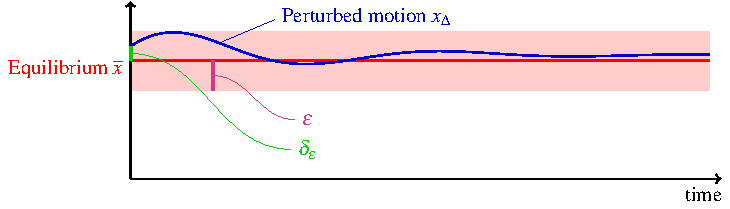
\includegraphics[width=0.60\columnwidth]{./Unit-02/img/StableEq-general.pdf}
            \end{center}
\item If the above does not hold true, the equilibrium is \TC{unstable}.
\end{itemize}
\end{frame}

\begin{frame}
\frametitleTC{Stability}
\framesubtitleTC{Asymptotically stable equilibrium}
\myPause
\begin{itemize}[<+-| alert@+>]
\item An equilibrium $\overline{x}$ corresponding to $\overline{u}$ is said to be \TC{asymptotically stable} if
      \begin{itemize}[<+-| alert@+>]
      \item it is stable,
      \item and \underline{in addition}
            \begin{displaymath}
             \lim_{k\rightarrow\infty} ||x_{\Delta}(k)-\overline{x}||=0.
            \end{displaymath}
      \end{itemize}
      \item Graphically,
            \begin{center}
             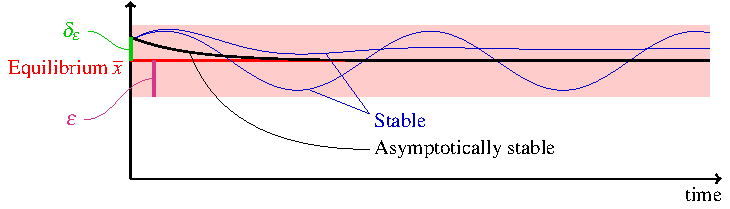
\includegraphics[width=0.60\columnwidth]{./Unit-02/img/AsympStableEq-general.pdf}
            \end{center}
\item Clearly asymptotic stability implies stability, but not \emph{vice versa}.
\end{itemize}
\end{frame}


\section{DT LTI -- state space}

\subsection{}

\begin{frame}
\frametitleTC{The DT LTI class}
\framesubtitleTC{Preliminaries}
\begin{itemize}[<+-| alert@+>]
\item For the LTI class, that we see here almost exclusively in the DT context, there exists a very strong theory.
\item The same is not true for more general (e.g., nonlinear) system classes.
\item Therefore, control problems of the type addressed here, are cast in the LTI framework wherever possible.
\item \vfill This motivates the importance of the DT LTI class, which we now\\
      come to examine.
\end{itemize}
\end{frame}

\begin{frame}
\frametitleTC{State-space representation of a DT LTI system}
\framesubtitleTC{Definition --- we stick to the SISO case for simplicity}
\myPause
\begin{itemize}[<+-| alert@+>]
\item The \TC{State-Space (SS)} representation of a DT LTI dynamic system is the quadruplet $(A,b,c,d)$ in
      \begin{displaymath}
       \left\{
        \begin{array}{rlll}
         x(k) &= A x(k-1) + b u(k-1) & & \text{\TC{(state equation)}}  \\
         y(k) &= c x(k)   + d u(k)   & & \text{\TC{(output equation)}}
        \end{array}
       \right.
      \end{displaymath}    
\item $u(k)$ and $y(k)$ are real scalars;
\item $x(k) \in \Re^n$, where $n$ is the system's order;
\item the real \TC{dynamic matrix} $A$ is $n \times n$;
\item $b$ is a real column vector ($n \times 1$);
\item $c$ is a real row vector ($1 \times n$);
\item $d$ is a real scalar.
\end{itemize}
\end{frame}

\begin{frame}
\frametitleTC{Motion}
\framesubtitleTC{}
\myPause
\begin{itemize}[<+-| alert@+>]
\item Given $x(0)$ and $u(k)$, $k \geq 0$, we get
      {\small
      \begin{displaymath}
       \begin{array}{rclcl}
        x(1) &=& Ax(0)+bu(0) \\
        x(2) &=& Ax(1)+bu(1) &=& A^2x(0)+Abu(0)+bu(1) \\
        x(3) &=& Ax(2)+bu(2) &=& A^3x(0)+A^2bu(0)+Abu(1)+bu(2) \\
             & & \cdots\\
       \end{array}
      \end{displaymath}
      }
\item This readily generalises to the \TC{Lagrange state formula}
      \begin{displaymath}
       x(k) = A^k x(0) +\sum\limits_{h=0}^{k-1} A^{k-h-1}bu(h).
      \end{displaymath}
\end{itemize}
\end{frame}

\begin{frame}
\frametitleTC{Free and induced state motion}
\framesubtitleTC{}
\myPause
\begin{itemize}[<+-| alert@+>]
\item In LTI systems, the state motion $x(k)$ is the \TC{sum} of a \TC{free motion} $x_F(k)$ and an
      \TC{induced motion} $x_I(k)$, i.e.,
      \begin{displaymath}
       x(k) = x_F(k) + x_I(k),
      \end{displaymath} \myPause
      where
      \begin{displaymath}
       x_F(k) = A^k x(0), \quad
       x_I(k) = \sum\limits_{h=0}^{k-1} A^{k-h-1}bu(h).
      \end{displaymath} \myPause
\item $x_F(k)$ depends linearly on $x(0)$ and not on $u$,
\item while $x_I(k)$ depends linearly only on $u(k)$ and not on $x(0)$.
\end{itemize}
\end{frame}

\begin{frame}
\frametitleTC{Free and induced output motion}
\framesubtitleTC{}
\myPause
\begin{itemize}[<+-| alert@+>]
\item In LTI systems, also the state motion $y(k)$ is the \TC{sum} of a \TC{free motion} $y_F(k)$ and an
      \TC{induced motion} $y_I(k)$, i.e.,
      \begin{displaymath}
       y(k) = y_F(k) + y_I(k),
      \end{displaymath} \myPause
      where
      \begin{displaymath}
       y_F(k) = cA^k x(0), \quad
       y_I(k) = c\sum\limits_{h=0}^{k-1} A^{k-h-1}bu(h) +du(k).
      \end{displaymath} \myPause
\item again, $y_F(k)$ depends linearly on $x(0)$ and not on $u$,
\item while $y_I(k)$ depends linearly only on $u(k)$ and not on $x(0)$.
\end{itemize}
\end{frame}

\begin{frame}
\frametitleTC{Equilibrium}
\framesubtitleTC{}
\myPause
\begin{itemize}[<+-| alert@+>]
\item For an LTI system, equilibrium states are found by solving
      \begin{displaymath}
       \overline{x} = A\overline{x}+b\overline{u}.
      \end{displaymath}
\item Thus, if $A$ has no unity eigenvalues, there exists the one equilibrium
      \begin{displaymath}
       \overline{x} = (I-A)^{-1}b\overline{u},
      \end{displaymath}
\item while in the opposite case, either there is no equilibrium, or there\\
      are infinite ones.
\end{itemize}
\end{frame}

\begin{frame}
\frametitleTC{Equilibrium}
\framesubtitleTC{Peculiarities of L(TI) systems}
\myPause
\begin{itemize}[<+-| alert@+>]
\item Contrary to nonlinear systems, they cannot have a finite number of equilibria, different from zero and one.
\item If some $\overline{u}$ produces zero, one or infinite equilibria, the same is true for any other $\overline{u}$,
      contrary again to the nonlinear case.
\item For each equilibrium state, there surely exists the one equilibrium output
      \begin{displaymath}
       \overline{y}=c\overline{x}+d\overline{u}.
      \end{displaymath}
\end{itemize}
\end{frame}

\begin{frame}
\frametitleTC{Stability of an equilibrium}
\framesubtitleTC{}
\myPause
\begin{itemize}[<+-| alert@+>]
\item Let $(\overline{x},\overline{u})$ be an equilibrium for an LTI system. 
\item The Lagrange state formula leads to write
      \begin{displaymath}
       \overline{x} = A^k \overline{x} +\sum\limits_{h=0}^{k-1} A^{k-h-1}b\overline{u}.
      \end{displaymath}.
\item Consider now the  perturbed motion $x_{\Delta}(k)$ produced by $\overline{u}$ and
      $x(0)=\overline{x}+\Delta\overline{x}$; the same formula yields
      \begin{displaymath}
       x_{\Delta}(k) = A^k (\overline{x}+\Delta\overline{x}) +\sum\limits_{h=0}^{k-1} A^{k-h-1}b\overline{u}.
      \end{displaymath}
\item Subtracting, therefore,
      \begin{displaymath}
       x_{\Delta}(k)-\overline{x} = A^k\Delta\overline{x}
      \end{displaymath}
\end{itemize}
\end{frame}

\begin{frame}
\frametitleTC{Stability of an equilibrium}
\framesubtitleTC{and in the L(TI) case, of a system}
\myPause
\begin{itemize}[<+-| alert@+>]
\item The way $x_{\Delta}(k)$ moves with respect to $\overline{x}$ does not depend on $\overline{x}$.
\item That is, contrary the nonlinear case, there cannot be equilibria with different stability characteristics.
\item In the L(TI) class, stability is a property of the \emph{system}, not of the individual equilibria.
\item Moreover, 
      \begin{itemize}[<+-| alert@+>]
      \item for $k\rightarrow\infty$, $||x_{\Delta}(k)-\overline{x}|| \rightarrow 0 \, \forall x(0)$  iff $A^k$
            converges to a zero matrix,
      \item the same norm generally diverges if at least one element of $A^k$ does,
      \item and if $A^k$ neither converges to zero nor diverges, the same happens\\
            to $||x_{\Delta}(k)-\overline{x}||$.
      \end{itemize}
\item Thus, in the LTI case, the stability of a system only depends on its\\
      dynamic matrix $A$.
\end{itemize}
\end{frame}

\begin{frame}[label={pag:stab-eivals}]
\frametitleTC{Stability and eigenvalues of $A$}
\framesubtitleTC{}
\myPause
\begin{itemize}[<+-| alert@+>]
\item The following can be proven.
      \begin{itemize}[<+-| alert@+>]
      \item An LTI system is asymptotically stable iff all the eigenvalues of $A$ have magnitude less  than one
            (or, equivalently, lie in the open \TC{unit circle} of the complex plane).
      \item The same system is unstable if (but not only if) at least one eigenvalue of $A$ has magnitude greater
            than one.
      \item If all the eigenvalues of $A$ have magnitude less than or equal to one, and there exists at least one
            with unity magnitude, the system can be either unstable\\
            or stable, but not asymptotically.
      \end{itemize}
\end{itemize}
\end{frame}

\begin{frame}
\frametitleTC{Properties of asymptotically stable systems}
\framesubtitleTC{also in a view to control}
\myPause
\begin{itemize}[<+-| alert@+>]
\item An asymptotically stable system has one and only one equilibrium for each constant input.
\item The state and output free motions of an asymptotically stable system converge to zero (norm)
      for $k\rightarrow\infty$.
\item As a consequence, asymptotically stable systems ``forget their initial condition''...
\item ...which is a definitely desired property for a \TC{controlled} system.
\end{itemize}
\end{frame}


\section{DT LTI -- transfer function and block diagrams}

\subsection{}

\begin{frame}
\frametitleTC{Preliminary}
\framesubtitleTC{for an alternative system representation, particularly useful for control}
\myPause
 \begin{itemize}[<+-| alert@+>]
 \item Let us introduce the \TC{one-step advance operator} $z$:
       \begin{displaymath}
        z\nu(k) := \nu(k+1) \qquad\qquad \text{whatever $\nu$ is}.
       \end{displaymath}
 \item This allows for a compact way to write LTI systems without evidencing the state (but it is there!).
 \item Suppose for example that we have a system with input $u$ and output $y$, ruled by
       \begin{displaymath}
        y(k) = ay(k-1)+bu(k-1),
       \end{displaymath}
       where clearly the state is the previous value of $y$;
 \item we can re-write $y(k+1)=ay(k)+bu(k)$ in the form
       \begin{displaymath}
        (z-a)y(k) = bu(k).
       \end{displaymath}
 \end{itemize}
\end{frame}

\begin{frame}
\frametitleTC{Preliminary}
\framesubtitleTC{introducing the transfer function}
\myPause
 \begin{itemize}[<+-| alert@+>]
 \item Rearranging -- remember the \emph{operatorial} meaning of $z$ -- we get
       \begin{displaymath}
        y(k) = \frac{b}{z-a}u(k)
       \end{displaymath}
\item[] and we can define the \TC{Transfer Function (TF)} notation, that expresses the system\\
        as a compound operator built upon the elementary one $z$:
       \begin{itemize}[<+-| alert@+>]
       \item we write the system's transfer function $G(z)$ as
             \begin{displaymath}
               G(z) = \frac{b}{z-a},
             \end{displaymath}
       \item[] and in force of this
             \begin{displaymath}
              y(k) = G(z)u(k) \quad \text{means} \quad y(k) = ay(k-1)+bu(k-1).
             \end{displaymath}
       \end{itemize}
 \item \vfill May not look so useful at the moment, but you will see later on\\
       how handy transfer functions are to determine controllers.
 \end{itemize}
\end{frame}

\begin{frame}
\frametitleTC{State space representation and transfer function}
\framesubtitleTC{}
\myPause
 \begin{itemize}[<+-| alert@+>]
 \item Given the SS representation we saw, shift all times by one (which is legit as the system is TI):
       \begin{displaymath}
        \left\{
         \begin{array}{rlll}
          x(k+1) &= A x(k)   + b u(k)\\
          y(k+1) &= c x(k+1) + d u(k+1) 
         \end{array}
        \right.
       \end{displaymath} 
 \item Apply the advance operator:
       \begin{displaymath}
        \left\{
         \begin{array}{rl}
          \textcolor{red}{z}x(k) &= A x(k) + b u(k)\\
          \textcolor{red}{z}y(k) &= c \textcolor{red}{z}x(k) + d\textcolor{red}{z} u(k)
         \end{array}
        \right.
       \end{displaymath} 
 \item Drop useless $z$'s and rearrange ($I$ is identity matrix of dimension $n$):
       \begin{displaymath}
        \left\{
         \begin{array}{rl}
          (zI-A)x(k) &= b u(k)\\
          y(k)       &= c x(k) + d u(k)
         \end{array}
        \right.
       \end{displaymath} 
 \end{itemize}
\end{frame}

\begin{frame}
\frametitleTC{State space representation and transfer function}
\framesubtitleTC{once again, sticking to the SISO case}
\myPause
 \begin{itemize}[<+-| alert@+>]
 \item Solve state equation for $x(k)$:
       \begin{displaymath}
        x(k) = (zI-A)^{-1} b u(k)
       \end{displaymath} 
 \item Substitute into output equation and rearrange:
       \begin{displaymath}
        y(k) = \textcolor{red}
                         {\underbrace{\left[c(zI-A)^{-1} b +d \right]}
                                    _{\text{Transfer function } G(z)}
                         } \; u(k)
       \end{displaymath} 
 \item We then define the transfer function of the generic SISO DT LTI\\
       system $(A,b,c,d)$ as
       \begin{displaymath}
        G(z) = c(zI-A)^{-1} b +d.
       \end{displaymath} 
 \end{itemize}
\end{frame}

\begin{frame}
\frametitleTC{Block diagrams}
\framesubtitleTC{Preliminaries}
\myPause
\begin{itemize}[<+-| alert@+>]
\item Block diagrams (BDs) are a graphical formalism to represent dynamic systems, that we see here limited to the
      DT LTI class.
\item They are useful to study \TC{interconnected} systems, i.e., compounds of \TC{subsystems} (e.g., a controller
      and the controlled object).
\item Important \emph{caveat}, that we state right from the beginning:
      \begin{itemize}[<+-| alert@+>]
      \item    a BD MUST NOT BE CONFUSED with a flow diagram;
      \item [] although subsystems have inputs and outputs,
      \item [] their compound comes from assembling \TC{equations}.
      \end{itemize}
\end{itemize}
\end{frame}

\begin{frame}
\frametitleTC{Block diagram components}
\framesubtitleTC{Block and summation node}
\myPause
\begin{center}
 \begin{picture}(210,70)(0,0)
  \put(000,35){\vector(1,0){30}}
  \put(000,40){{\small $u(k)$}}
  \put(030,20){\framebox(50,30)
              {$G(z)$}
              }
  \put(080,35){\vector(1,0){30}}
  \put(090,40){{\small $y(k)$}}

  \put(175,35){\circle{10}}

  \put(175,70){\vector(0,-1){30}}
  \put(150,62){{\small $u_1(k)$}}
  \put(165,40){{\small $+$}}

  \put(140,35){\vector(1,0){30}}
  \put(140,40){{\small $u_2(k)$}}
  \put(162,27){{\small $-$}}

  \put(175,00){\vector(0,1){30}}
  \put(150,03){{\small $u_3(k)$}}
  \put(167,20){{\small $+$}}

  \put(180,35){\vector(1,0){30}}
  \put(190,40){{\small $y(k)$}}
\end{picture}

\end{center} \myPause
\begin{itemize}[<+-| alert@+>]
\item \TC{Block} (left):\\
      an LTI SISO system with the indicated transfer function -- in the shown\\
      example, the \TC{equation} $G(z)u(k)-y(k)=0$.
\item \TC{Summation node} (right):\\
      a summation expression -- in the shown example, the \TC{equation}
      $u_1(k)-u_2(k)+u_3(k)-y(k)=0$.
\end{itemize}
\end{frame}


\section{Conclusions}
\subsection{}

\begin{frame}
\frametitleTC{Conclusions}
\framesubtitleTC{Recap and lessons learnt (1/2)}
\myPause
 \begin{itemize}[<+-| alert@+>]
 \item We can characerise a dynamic system with \TC{time domain responses}.
 \item These refer to a certain \emph{stimulus} (we used impulse and step).
 \item Responses can be used also to stipulate \TC{control objectives}.
 \item A viable way to do so is to transform time domain deires into some desired
       closed-loop transfer function.
 \item This paves the way to the \TC{direct synthesis} technique.
 \end{itemize}
\end{frame}

\begin{frame}
\frametitleTC{Conclusions}
\framesubtitleTC{Recap and lessons learnt (2/2)}
\myPause
 \begin{itemize}[<+-| alert@+>]
 \item We have open issues, however.
       \begin{itemize}[<+-| alert@+>]
       \item Why impulse and step \emph{stimuli} are meaningful?
       \item How can we choose the target closed-loop transfer function?
       \item What are the limits and what is their origin?
       \end{itemize}
 \item \vfill These issues are very suited for addressing in a practice session,\\
       which is our next task.
 \item Please review your notes, next time ask questions if needed\\
       before we start.
 \end{itemize}
\end{frame}

\section{}
{
\setbeamertemplate{headline}{
  \begin{beamercolorbox}[wd=\paperwidth,ht=4.2ex,dp=1.5ex]{palette quaternary}
  \end{beamercolorbox}
  }
\setbeamertemplate{footline}{
  \begin{beamercolorbox}[wd=\paperwidth,ht=2.2ex,dp=1.5ex]{palette quaternary}
  \end{beamercolorbox}
  }
\begin{frame}[noframenumbering]
 \vspace{20mm}\Huge{Discussion open}
\end{frame}
}



%%% UNIT 3
{
\setbeamertemplate{headline}{}
\setbeamertemplate{footline}{
  \begin{beamercolorbox}[wd=\paperwidth,ht=2.2ex,dp=1.5ex]{palette quaternary}
  \end{beamercolorbox}
  }
\begin{frame}[noframenumbering]
\frametitle{\DB{\huge{\textbf{$\blacksquare$ Unit 3}}}}
\myPause
 \begin{itemize}
 \item[] \LARGE{\MB{Practice session 1}}
 \item[] \vspace{-1mm}\hspace{5mm}\Large{\MB{Dynamic systems}}
 \end{itemize}
\end{frame}
}

\part{}

\section{Exercise 01}
\subsection{}

\begin{frame}
\frametitleTC{Problem}
\framesubtitleTC{This one we solve together}
\myPause
 Given the DT LTI dynamic system described in the state space by
 \begin{displaymath}
  A = \begin{bmatrix} 0.4 & 0.4 \\ 0.05 & 0.3 \end{bmatrix}, \quad
  b = \begin{bmatrix} 1 \\ 0.5 \end{bmatrix}, \quad
  c = \begin{bmatrix} 2 & -1 \end{bmatrix}, \quad
  d = 0,
 \end{displaymath}
 \begin{itemize}[<+-| alert@+>]
 \item[(a)] discuss its stability,
 \item[(b)] express it in scalar form,
 \item[(c)] compute its transfer function,
 \item[(d)] compute the first three values ($k=0,1,2$) of its response to
            \begin{displaymath}
             x(0) = \begin{bmatrix} 2 \\ 1 \end{bmatrix}, \quad
             u(k) = 0.4k.
            \end{displaymath}
 \end{itemize}
\end{frame}

\begin{frame}
\frametitleTC{Solution}
\framesubtitleTC{Item (a)}
\myPause
 \begin{itemize}[<+-| alert@+>]
 \item We need to compute the eigenvalues $\lambda_{1,2}$ of $A$:
       \begin{itemize}[<+-| alert@+>]
       \item[] \vspace{1mm}
               $\det(\lambda I -A) = 0$,
       \item[] \vspace{1mm}
               $\det \left(
                     \begin{bmatrix} \lambda & 0 \\ 0 & \lambda \end{bmatrix}
                    -\begin{bmatrix} 0.4 & 0.4 \\ 0.05 & 0.3 \end{bmatrix}
                     \right) = 0 $,
       \item[] \vspace{1mm}
               $\det \begin{bmatrix} \lambda-0.4 & -0.4 \\
                                    -0.05       & \lambda-0.3 \end{bmatrix} = 0 $,
       \item[] \vspace{1mm}
               $(\lambda-0.4)(\lambda-0.3)-(-0.4)(-0.05) = 0$,
       \item[] \vspace{1mm}
               $\lambda^2-0.7\lambda+0.1=0$,
       \item[] \vspace{1mm}
               $\lambda=\cfrac{0.7\mp\sqrt{0.7^2-4\cdot 0.5}}{2} \quad \Rightarrow \quad
                \lambda_1=0.2, \; \lambda_2=0.5.$
       \end{itemize}
 \item All the eigenvalues of $A$ are strictly less than one in magnitude\\
       $\Rightarrow$ the system is asymptotically stable.
 \end{itemize}
\end{frame}

\begin{frame}
\frametitleTC{Solution}
\framesubtitleTC{Item (b)}
\myPause
 \begin{itemize}[<+-| alert@+>]
 \item Denoting by $x=[x_1\;x_2]'$ the state vector (sign $'$means transpose) we have
       \begin{displaymath}
        \left\{\begin{array}{rcl}
         \begin{bmatrix} x_1(k) \\ x_2(k) \end{bmatrix} 
         &=&             
         \begin{bmatrix} 0.4 & 0.4 \\ 0.05 & 0.3 \end{bmatrix}\,
         \begin{bmatrix} x_1(k-1) \\ x_2(k-1) \end{bmatrix}
         +
         \begin{bmatrix} 1 \\ 0.5 \end{bmatrix}\,
         u(k-1) \\
         y(k)
         &=&          
         \begin{bmatrix} 2 & -1 \end{bmatrix} \,
         \begin{bmatrix} x_1(k) \\ x_2(k) \end{bmatrix}
        \end{array}\right.
       \end{displaymath}
 \item hence in scalar form
       \begin{displaymath}
        \left\{\begin{array}{rcl}
         x_1(k) &=&  0.4 x_1(k-1) + 0.4 x_2(k-1) +    u(k-1)\\
         x_2(k) &=& 0.05 x_1(k-1) + 0.3 x_2(k-1) + 0.5u(k-1)\\
         y(k)   &=&    2 x_1(k-1) -     x_2(k-1)
        \end{array}\right.
       \end{displaymath}
 \end{itemize}
\end{frame}

\begin{frame}
\frametitleTC{Solution}
\framesubtitleTC{Item (c)}
\myPause
 \begin{itemize}[<+-| alert@+>]
 \item The transfer function $G(z)$ is $c(zI-A)^{-1}b+d$, hence
       \begin{itemize}
       \item[] \begin{itemize}[<+-| alert@+>]
               \item[$G(z)$] \vspace{1mm}
                    $= \begin{bmatrix} 2 & -1 \end{bmatrix} \,
                       \begin{bmatrix} z-0.4 & -0.4 \\
                       -0.05& z-0.3 \end{bmatrix}^{-1} \,
                       \begin{bmatrix} 1 \\ 0.5 \end{bmatrix}
                       +0
                    $
               \item[] \vspace{1mm}
                    $= \cfrac{1}{(z-0.5)(z-0.2)}
                       \begin{bmatrix} 2 & -1 \end{bmatrix} \,
                       \begin{bmatrix} z-0.3 & 0.4 \\
                       0.05& z-0.4 \end{bmatrix} \,
                       \begin{bmatrix} 1 \\ 0.5 \end{bmatrix}
                    $
               \item[] \vspace{1mm}
                    $= \cfrac{1}{(z-0.5)(z-0.2)}
                       \begin{bmatrix} 2z-0.65 &-z+1.2 \end{bmatrix} \,
                       \begin{bmatrix} 1 \\ 0.5 \end{bmatrix}
                    $
               \item[] \vspace{1mm}
                    $= \cfrac{1.5z-0.05}{(z-0.5)(z-0.2)}.
                    $
               \end{itemize}
       \end{itemize}
 \end{itemize}
\end{frame}

\begin{frame}
\frametitleTC{Solution}
\framesubtitleTC{Item (d)}
\myPause
 \begin{itemize}[<+-| alert@+>]
 \item We have\\
       $u(0) = 0, \quad u(1) = 0.4, \quad u(2) = 0.8, \quad u(3) = 1.2, \, \ldots$
 \item We need to iteratively apply the state and output equations, whence
       \begin{itemize}
       \item[] \begin{itemize}[<+-| alert@+>]
               \item[$k=0$:] \vspace{1mm} 
                    $\left\{\begin{array}{rll}
                     x(0) &= \begin{bmatrix} 2 \\ 1 \end{bmatrix} (\text{given}) \\
                     y(0) &= \begin{bmatrix} 2 & -1 \end{bmatrix} \,
                             \begin{bmatrix} 2 \\ 1 \end{bmatrix}
                          &= 3
                     \end{array}\right.
                    $
               \item[$k=1$:] \vspace{1mm} 
                    $\left\{\begin{array}{rll}
                     x(1) &= \begin{bmatrix} 0.4 & 0.4 \\ 0.05 & 0.3 \end{bmatrix} \,
                             \begin{bmatrix} 2 \\ 1 \end{bmatrix}
                            +\begin{bmatrix} 1 \\ 0.5 \end{bmatrix} \cdot 0
                          &= \begin{bmatrix} 1.2 \\ 0.4 \end{bmatrix}\\
                     y(1) &= \begin{bmatrix} 2 & -1 \end{bmatrix} \,
                             \begin{bmatrix} 1.2 \\ 0.4 \end{bmatrix}
                          &= 2
                     \end{array}\right.
                    $
               \item[$k=2$:] \vspace{1mm} 
                    $\left\{\begin{array}{rll}
                     x(1) &= \begin{bmatrix} 0.4 & 0.4 \\ 0.05 & 0.3 \end{bmatrix} \,
                             \begin{bmatrix} 1.2 \\ 0.4 \end{bmatrix}
                            +\begin{bmatrix} 1 \\ 0.5 \end{bmatrix} \cdot 0.4
                          &= \begin{bmatrix} 1.04 \\ 0.38 \end{bmatrix}\\
                     y(1) &= \begin{bmatrix} 2 & -1 \end{bmatrix} \,
                             \begin{bmatrix} 1.04 \\ 0.38 \end{bmatrix}
                          &= 1.7
                     \end{array}\right.
                    $
               \end{itemize}
       \end{itemize}
 \end{itemize}
\end{frame}

\begin{frame}
\frametitleTC{Addendum}
\framesubtitleTC{}
\myPause
 \begin{itemize}[<+-| alert@+>]
 \item We define some signals useful for the following.
       \begin{itemize}[<+-| alert@+>]
       \item Impulse (precisely, \TC{unit} impulse as the value is 1):
             \begin{displaymath}
              imp(k) = \begin{cases} 1 & k=0 \\ 0 & \text{otherwise} \end{cases}
             \end{displaymath}
       \item Step (\TC{unit} step, amplitude is 1):
             \begin{displaymath}
              step(k) = \begin{cases} 1 & k \geq 0 \\ 0 & \text{otherwise} \end{cases}
             \end{displaymath}
       \item Ramp(\TC{unit} ramp, slope is 1):
             \begin{displaymath}
              ramp(k) = k\; step(k) = \begin{cases} k & k \geq 0 \\ 0 & \text{otherwise} \end{cases}
             \end{displaymath}
       \end{itemize}
 \item Quite frequently ``unit'' is omitted, e.g. ``step response'' actually\\
       means ``unit step response''.
 \end{itemize}
\end{frame}

\begin{frame}
\frametitleTC{Proposed exercise 01}
\framesubtitleTC{Try this at home, ask questions next time if needed}
\myPause
 Given the DT LTI dynamic system described in the state space by
 \begin{displaymath}
  A = \begin{bmatrix} 0.5 & 0 \\ 2 & -0.3 \end{bmatrix}, \quad
  b = \begin{bmatrix} 1 \\ 0 \end{bmatrix}, \quad
  c = \begin{bmatrix} 0 & 4 \end{bmatrix}, \quad
  d = 1,
 \end{displaymath}
 \begin{itemize}[<+-| alert@+>]
 \item[(a)] discuss its stability,
 \item[(b)] express it in scalar form,
 \item[(c)] compute its transfer function,
 \item[(d)] compute the first three values ($k=0,1,2$) of its response to
            \begin{displaymath}
             x(0) = \begin{bmatrix} 1 \\ 1 \end{bmatrix}, \quad
             u(k) = 2 step(k).
            \end{displaymath}
 \end{itemize}
\end{frame}

\begin{frame}[fragile]
\frametitleTC{But how can we check our results?}
\framesubtitleTC{}
\myPause
 \begin{itemize}[<+-| alert@+>]
 \item With the symbolic package wxMaxima:
       \begin{verbatim}
        A  : matrix([0.4,0.4],[0.05,0.3]);
        b  : matrix([1],[0.5]);
        c  : matrix([2,-1]);
        d  : 0;
        G  : factor(c.invert(z*ident(2)-A).b+d);
        Gr : rat(G,z);
        x0 : matrix([2],[1]);
        y0 : c.x0;
        x1 : A.x0+b*0;   /* the 0   is u(0) */
        y1 : c.x1;
        x2 : A.x1+b*0.4; /* the 0.4 is u(1) */
        y2 : c.x2;
       \end{verbatim}

 \end{itemize}
\end{frame}

\begin{frame}
\frametitleTC{But how can we check our results?}
\framesubtitleTC{}
\myPause
 \begin{itemize}[<+-| alert@+>]
 \item We are learning (the bit we need of) wxMaxima by example.
 \item For the moment:
       \begin{itemize}[<+-| alert@+>]
       \item you SET with \texttt{:}, \texttt{=} is for equations,
       \item \texttt{[} and \texttt{]} delimit a list,
       \item matrices are defined with \texttt{matrix} as one list per row,
       \item you multiply scalars (or by a scalar) with \texttt{*}, matrices \& vectors with \texttt{.} (period), 
       \item \texttt{ident(n)} is identity of dimension n,
       \item \texttt{invert} is self-explanatory, you also have \texttt{transpose}, \texttt{determinant},\\
             \texttt{eigenvalues}, \texttt{eigenvectors} and much more,
       \item \texttt{factor} attempts to factor an expression, \texttt{rat(expr,var)} to express\\
             \texttt{expr} rationally wrt \texttt{var};
       \item enjoy \smiley...
       \end{itemize}
 \end{itemize}
\end{frame}

\begin{frame}
\frametitleTC{Takeaways}
\framesubtitleTC{from exercise 01 (and the proposed one)}
\myPause
 \begin{itemize}[<+-| alert@+>]
 \item A transfer function is the ratio of two polynomials.
 \item We call the roots of its numerator the \TC{zeroes}.
 \item We call the roots of its denominator the \TC{poles}. 
 \item The poles are eigenvalues of $A$.
 \item The degree of the numerator is at most equal to that of the denominator,
 \item and equal iff $d \neq 0$ (you will see this in the proposed exercise, try to\\
       prove it holds true in general).
 \item We call the number of poles minus that of zeroes the \TC{relative degree}\\
       of the system.
 \end{itemize}
\end{frame}


\section{Exercise 02}
\subsection{}

\begin{frame}
\frametitleTC{Problem}
\framesubtitleTC{This one we solve together}
\myPause
 Take the same system as in exercise 01, i.e.,
 \begin{displaymath}
  A = \begin{bmatrix} 0.4 & 0.4 \\ 0.05 & 0.3 \end{bmatrix}, \quad
  b = \begin{bmatrix} 1 \\ 0.5 \end{bmatrix}, \quad
  c = \begin{bmatrix} 2 & -1 \end{bmatrix}, \quad
  d = 0,
 \end{displaymath}
 and turn it into a block diagram.\\ \myPause
 \vspace{5mm}Important hint: since $z$ is the one-step advance operator, $z^{-1}$ is the one-step\\
 \emph{delay} operator, i.e., 
 \begin{displaymath}
  z^{-1} v(k) = v(k-1).
 \end{displaymath}
\end{frame}

\begin{frame}
\frametitleTC{Solution}
\framesubtitleTC{}
\myPause
 \only<2 >{One delay element per state variable:\\
           \begin{center}
            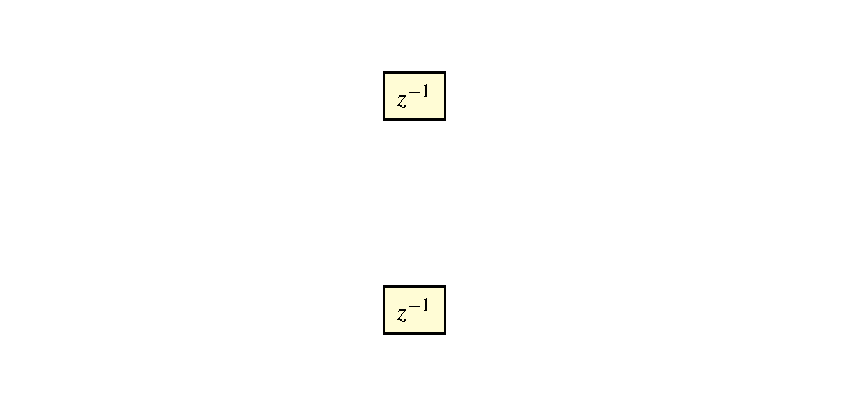
\includegraphics[width=0.85\columnwidth]{./Unit-03/img/PS01-ex02-fig01.pdf}
           \end{center}}
 \only<3 >{If the inputs are the $x_i(k+1)$, then the outputs are the $x_i(k)$:\\
           \begin{center}
            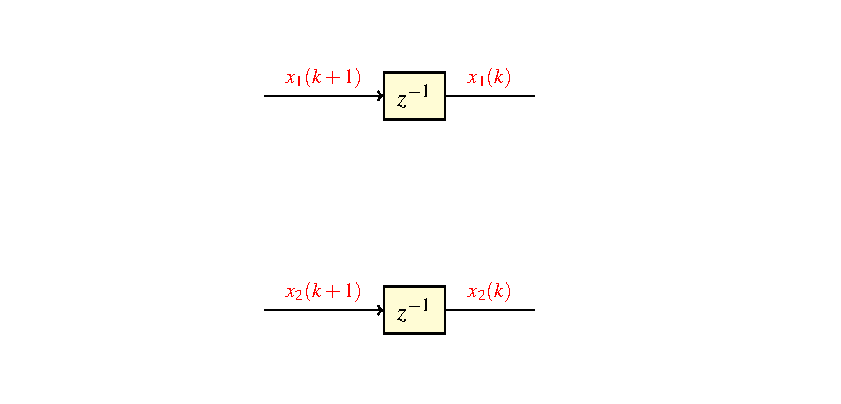
\includegraphics[width=0.85\columnwidth]{./Unit-03/img/PS01-ex02-fig02.pdf}
           \end{center}}
 \only<4 >{Now place the elements of \textcolor{magenta}{$A$} and \textcolor{blue}{$b$}:\\
           \begin{center}
            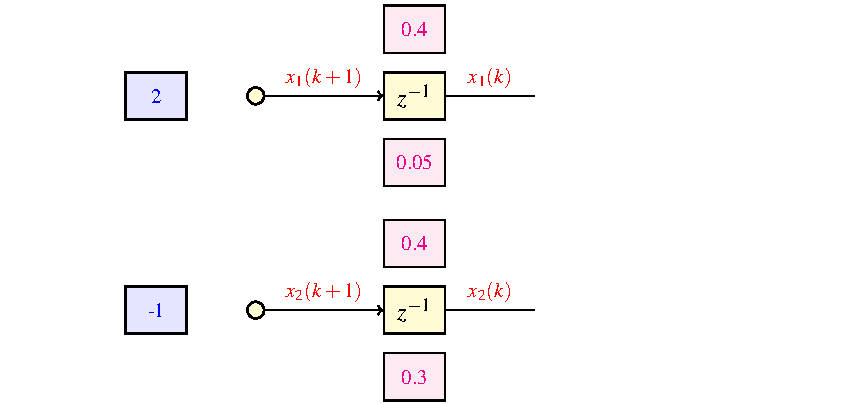
\includegraphics[width=0.85\columnwidth]{./Unit-03/img/PS01-ex02-fig03.pdf}
           \end{center}}
 \only<5 >{Read the state equation and wire how $x(k+1)$ depends on $x(k)$:\\
           \begin{center}
            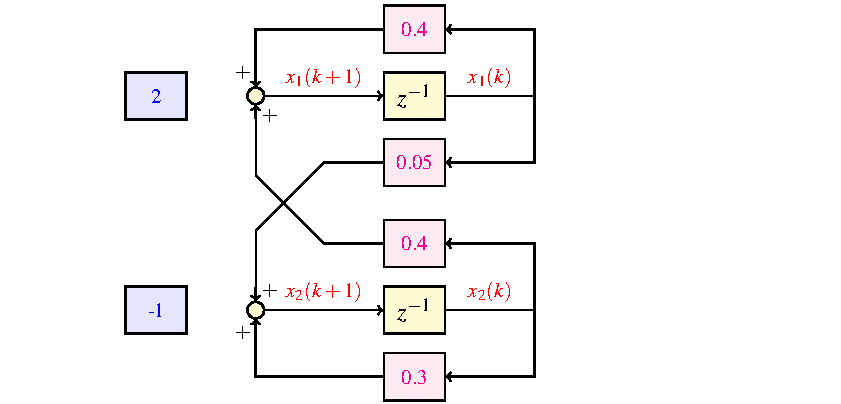
\includegraphics[width=0.85\columnwidth]{./Unit-03/img/PS01-ex02-fig04.pdf}
           \end{center}}
 \only<6 >{Continue reading and wire how $x(k+1)$ depends on $u(k)$:\\
           \begin{center}
            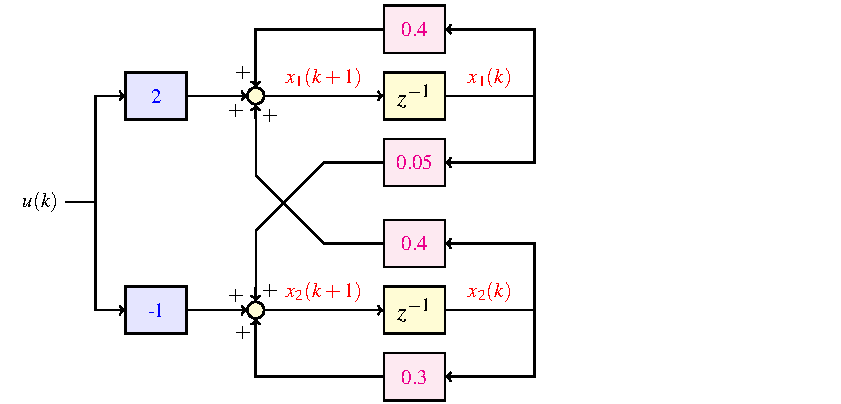
\includegraphics[width=0.85\columnwidth]{./Unit-03/img/PS01-ex02-fig05.pdf}
           \end{center}}
 \only<7 >{Now place the elements of \textcolor{green!80!black}{$c$}:\\
           \begin{center}
            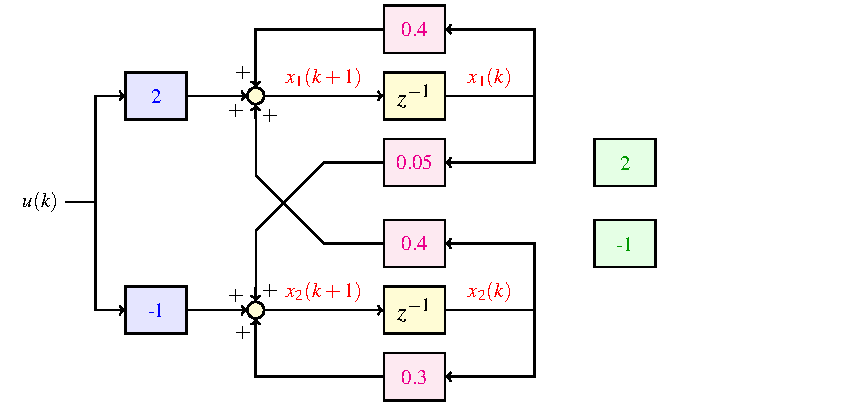
\includegraphics[width=0.85\columnwidth]{./Unit-03/img/PS01-ex02-fig06.pdf}
           \end{center}}
 \only<8->{Read the output equation and complete the block diagram:\\
           \begin{center}
            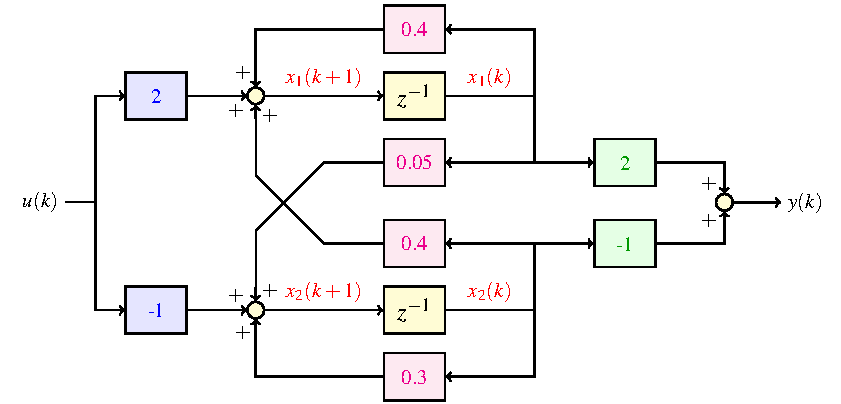
\includegraphics[width=0.85\columnwidth]{./Unit-03/img/PS01-ex02-fig07.pdf}
           \end{center}}
\end{frame}

\begin{frame}
\frametitleTC{Proposed exercise 02}
\framesubtitleTC{Try this at home, ask questions next time if needed}
\myPause
 Take the same system as in the previous proposed exercise, i.e.,
 \begin{displaymath}
  A = \begin{bmatrix} 0.5 & 0 \\ 2 & -0.3 \end{bmatrix}, \quad
  b = \begin{bmatrix} 1 \\ 0 \end{bmatrix}, \quad
  c = \begin{bmatrix} 0 & 4 \end{bmatrix}, \quad
  d = 1,
 \end{displaymath}
 and turn it into a block diagram.\\ \myPause
 \vspace{5mm}Remark: in this case you will see a \TC{direct feedthrough} from $u$ to $y$,\\
 because $d \neq 0$. 
\end{frame}

\begin{frame}
\frametitleTC{Takeaways}
\framesubtitleTC{from exercise 02 (and the proposed one)}
\myPause
 \begin{itemize}[<+-| alert@+>]
 \item Generalise the situation with compact matrix notation (thick lines are vectors):
       \begin{center}
        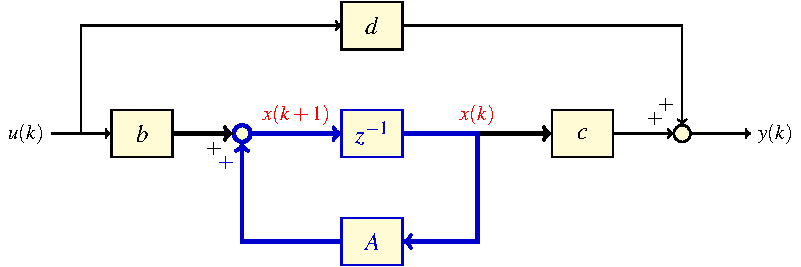
\includegraphics[width=0.65\columnwidth]{./Unit-03/img/PS01-ex02-takeaway-FBscheme.pdf}
       \end{center}
 \item Do you see the \textcolor{blue!80!black}{feedback loop} inherently inside the system?
 \item Feedback is not ``an invention for control''; it is an integral part\\
       of how nature works!
 \end{itemize}
\end{frame}

\begin{frame}
\frametitleTC{Takeaways}
\framesubtitleTC{from exercise 02 (and the proposed one)}
\myPause
 \begin{itemize}[<+-| alert@+>]
 \item Get acquainted with the $(k,k-1)$ and the $(k+1,k)$ ways of writing a DT system,\\
       and always pay attention to which symbol is what.
 \item In particular, the $u$ in the state equation is NOT at the same instant as that\\
       in the output equation, no matter how the system is written.
 \item \vspace{4mm}As feedback is a powerful weapon, ``slight'' approximations as taking\\
       the previous input of a block and not the current, or \emph{vice versa},\\
       can in fact be devastating...
 \item ...and without a system-theoretical analysis, this is impossible\\
       to figure out before the system is run --- i.e., possibly, broken.
 \end{itemize}
\end{frame}




\section{Exercise 03}
\subsection{}

\begin{frame}
\frametitleTC{Problem}
\framesubtitleTC{This one we solve together}
 Given the two DT LTI dynamic systems
 \begin{displaymath}
  S_1:
  \left\{\begin{array}{rcl}
   x_1(k) &=& 0.5x_1(k-1)+u(k-1)\\
   x_2(k) &=& 0.5x_2(k-1)+u(k-1)\\
   y(k)   &=& x_1(k)+x_2(k)
  \end{array}\right. \quad
  S_2:
  \left\{\begin{array}{rcl}
   x_1(k) &=& 0.4x_1(k-1)+u(k-1)\\
   x_2(k) &=& 0.8x_2(k-1)+u(k-1)\\
   y(k)   &=& x_2(k)
  \end{array}\right.
 \end{displaymath}

 \begin{itemize}[<+-| alert@+>]
 \item[(a)] compute their transfer functions,
 \item[(b)] comment on the result.
 \end{itemize}
\end{frame}

\begin{frame}
\frametitleTC{Solution}
\framesubtitleTC{Item (a)}
\myPause
 \begin{itemize}[<+-| alert@+>]
 \item We start with $S_1$:
       \begin{itemize}
       \item[] \begin{itemize}[<+-| alert@+>]
               \item[$G(z)$] \vspace{1mm}
                    $= \begin{bmatrix} 1 & 1  \end{bmatrix} \,
                       \begin{bmatrix} z-0.5 & 0 \\
                                       0     & z-0.5 \end{bmatrix}^{-1} \,
                       \begin{bmatrix} 1 \\ 1 \end{bmatrix}
                       +0
                    $
               \item[] \vspace{1mm}
                    $= \cfrac{1}{(z-0.5)^2}
                       \begin{bmatrix} 1 & 1 \end{bmatrix} \,
                       \begin{bmatrix} z-0.5 & 0 \\
                                       0     & z-0.5 \end{bmatrix} \,
                       \begin{bmatrix} 1 \\ 1 \end{bmatrix}
                    $
               \item[] \vspace{1mm}
                    $= \cfrac{1}{(z-0.5)^2}
                       \begin{bmatrix} z-0.5 & z-0.5 \end{bmatrix} \,
                       \begin{bmatrix} 1 \\ 1 \end{bmatrix}
                    $
               \item[] \vspace{1mm}
                    $= \cfrac{2\cancel{(z-0.5)}}{(z-0.5)^{\cancel{2}}} \qquad \qquad
                       \TC{\leftarrow \text{zero/pole \underline{cancellation}}}
                    $
               \item[] \vspace{1mm}
                    $= \cfrac{2}{z-0.5}.
                    $
               \end{itemize}
       \end{itemize}
 \end{itemize}
\end{frame}


\begin{frame}[fragile]
\frametitleTC{Solution}
\framesubtitleTC{Item (a)}
\myPause
 \begin{itemize}[<+-| alert@+>]
 \item And now $S_2$:
       \begin{itemize}
       \item[] \begin{itemize}[<+-| alert@+>]
               \item[] wxMaxima, we are lazy \smiley
                       \begin{verbatim}
A:matrix([0.4,0],[0,0.8]);
b:matrix([1],[1]);
c:matrix([0,1]);
G:c.invert(z*ident(2)-A).b;
                       \end{verbatim}
               \item[] \vspace{1mm}
                    $ G(z) = \cfrac{1}{z-0.8}.
                    $
               \end{itemize}
               \item \vspace{3mm}Another case with cancellation: the characteristic polynomial of $A$\\
                     has degree 2, the denominator of $G(z)$ has degree 1.
       \end{itemize}
 \end{itemize}
\end{frame}



\begin{frame}
\frametitleTC{Solution}
\framesubtitleTC{Item (b) -- comments on the $S_1$ case}
\myPause
 \begin{itemize}[<+-| alert@+>]
 \item In fact $S_1$ is a ``fake'' 2nd order system, since as far as induced motions are\\
       concerned  $x_1$ and $x_2$ are the same, and the system is \TC{input-output} (i.e, as far\\
       as we only look at $u$ and $y$) \TC{equivalent} to a 1st order one:
       \begin{displaymath}
        \left\{\begin{array}{rcl}
         x_1(k) &=& 0.5x_1(k-1)+u(k-1)\\
         x_2(k) &=& 0.5x_2(k-1)+u(k-1)\\
         y(k)   &=& x_1(k)+x_2(k)
        \end{array}\right. \quad
        \Rightarrow \quad
        \left\{\begin{array}{rcl}
         x(k) &=& 0.5x(k-1)+u(k-1)\\
         y(k) &=& 2x(k)
        \end{array}\right.
        \end{displaymath} 
        apparently with
        \begin{displaymath}
         G(z)=\cfrac{2}{z-0.5}.
        \end{displaymath} 
 \item This system cannot move in the whole $(x_1,x_2)$ plane, but only\\
       on the straight line $x_1=x_2$.
 \item In general, systems like this can only move on a \TC{subspace} (line)\\
       of their \TC{state space} (plane).
 \item We call them \TC{not fully reachable} (the term should be intuitive).
 \end{itemize}
\end{frame}

\begin{frame}
\frametitleTC{Solution}
\framesubtitleTC{Item (b) -- comments on the $S_2$ case}
\myPause
 \begin{itemize}[<+-| alert@+>]
 \item Also $S_2$ is a ``fake'' 2nd order system, because however $x_1$ moves, $y$ does not
       reveal this, and thus we can reduce this system as well to a 1st order one:
       \begin{displaymath}
        \left\{\begin{array}{rcl}
         x_1(k) &=& 0.4x_1(k-1)+u(k-1)\\
         x_2(k) &=& 0.8x_2(k-1)+u(k-1)\\
         y(k)   &=& x_2(k)
        \end{array}\right. \quad
        \Rightarrow \quad
        \left\{\begin{array}{rcl}
         x(k) &=& 0.8x(k-1)+u(k-1)\\
         y(k) &=& x(k)
        \end{array}\right.
        \end{displaymath} 
        apparently with
        \begin{displaymath}
         G(z)=\cfrac{1}{z-0.8}.
        \end{displaymath} 
 \item In this system one state variable does not influence the output.
 \item We call such systems \TC{not fully observable} (the term should be\\
       once again intuitive).
 \end{itemize}
\end{frame}

\begin{frame}
\frametitleTC{Proposed exercise 03}
\framesubtitleTC{Try this at home, ask questions next time if needed}
\myPause
 Take the two system of exercise 03, and turn them into block diagrams.\\
 \vspace{5mm}Analyse those diagrams along the idea that parts of the system are not influenced
 by the input, or do not influence the output. 
\end{frame}



\begin{frame}
\frametitleTC{Takeaways}
\framesubtitleTC{from exercise 03 (and the proposed one)}
\myPause
 \begin{itemize}[<+-| alert@+>]
 \item There are cases in which a system cannot move in all its state space, or equivalently,
       some state variables are not influenced by the input.
 \item Suggestion for reflections: why ``equivalently''?
 \item There are also cases in which some state variables do not influence the output.
 \item There are also cases where both facts occur.
 \item We detect this because in computing the transfer function we get\\
       \TC{cancellations}.
 \end{itemize}
\end{frame}

\begin{frame}
\frametitleTC{Takeaways}
\framesubtitleTC{from exercise 03 (and the proposed one)}
\myPause
 \begin{itemize}[<+-| alert@+>]
 \item Do we need to bother?
 \item Yes, because this collectively means that a system may have \TC{hidden parts}\\
       (things the transfer function does not tell).
 \item In setting up controls, we must be careful to not generate UNSTABLE hidden parts.
 \item We do not mind about asymptotically stable ones, because their effect\\
       vanishes with their free motion.
 \end{itemize}
\end{frame}




\section{Exercise 04}
\subsection{}

\begin{frame}[label={pag:ex-realisation}]
\frametitleTC{Problem}
\framesubtitleTC{This one we solve together}
\myPause
 Take the block diagram
 \begin{center}
  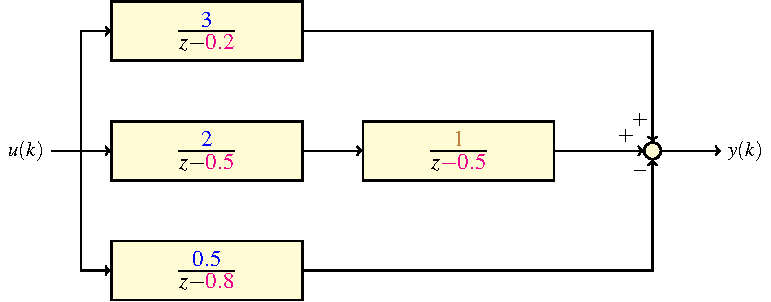
\includegraphics[width=0.85\columnwidth]{./Unit-03/img/PS01-ex04-fig01.pdf}
 \end{center}\myPause
 \begin{itemize}[<+-| alert@+>]
 \item[(a)] compute the transfer function from $u(k)$ to $y(k)$,
 \item[(b)] find a possible state-space description for the system.
 \end{itemize}
\end{frame}

\begin{frame}
\frametitleTC{Solution}
\framesubtitleTC{Item (a) -- preliminaries}
\myPause
 \begin{itemize}[<+-| alert@+>]
 \item Take two blocks in \TC{series} or \TC{cascade}, i.e., the output $y_1(k)$ of the first is the
       input $u_2(k)$ of the second. Name $G_1(z)$ and $G_2(z)$ their transfer functions.
 \item Let the overall system input $u(k)$ be connected to the input $u_1(k)$ of $G_1(z)$, and the overall
       system output $y(k)$ be the output $y_2(k)$ of $G_2(z)$.
 \item Then we have
       \begin{displaymath}
        y(k) = y_2(k) = G_2(z)u_2(k) = G_2(z)y_1(k) = G_2(z)G_1(z)u_1(k)=G_2(z)G_1(z)u(k),
       \end{displaymath}
 \item and therefore the overall transfer function $G(z)$ from $u(k)$ to $y(k)$ is
       \begin{displaymath}
        G(z) = G_2(z)G_1(z).
       \end{displaymath}
 \end{itemize}
\end{frame}

\begin{frame}
\frametitleTC{Solution}
\framesubtitleTC{Item (a) -- preliminaries}
\myPause
 \begin{itemize}[<+-| alert@+>]
 \item Take two blocks $G_1(z)$ and $G_2(z)$ in \TC{parallel}, i.e., they get the same input $u(k)$
       and their outputs sum together to produce the overall system output $y(k)$.
 \item With obvious notation have
       \begin{displaymath}
        y(k) = y_1(k)+y_2(k) = G_1(z)u_1(k)+G_2(z)u_2(k) = (G_1(z)+G_2(z))u(k),
       \end{displaymath}
 \item and therefore the overall transfer function $G(z)$ from $u(k)$ to $y(k)$ is
       \begin{displaymath}
        G(z) = G_1(z)+G_2(z).
       \end{displaymath}
 \item Extending to more blocks and different signs is trivial.
 \end{itemize}
\end{frame}

\begin{frame}
\frametitleTC{Solution}
\framesubtitleTC{Item (a)}
\myPause
 \begin{itemize}[<+-| alert@+>]
 \item The system under question is composed of three branches in parallel.
 \item The middle one is composed of two blocks in series.
 \item Hence (mind the signs) the overall transfer function $G(z)=y(k)/u(k)$ is
       \begin{displaymath}
        \begin{array}{rcll}
         G(z) &=& & \cfrac{3}{z-0.2}\\
              & &+& \cfrac{2}{z-0.5} \,\cdot\,
                    \cfrac{1}{z-0.5}\\
              & &-& \cfrac{0.5}{z-0.8} \; \ldots\\ \\
              &=& & \cfrac{2.5z^3-2.8z^2+0.925z-0.255}{(z-0.2)(z-0.5)^2(z-0.8)}.
        \end{array}
       \end{displaymath}
 \end{itemize}
\end{frame}

\begin{frame}
\frametitleTC{Solution}
\framesubtitleTC{Item (b)}
\myPause%
 \only<2 >{Consider the individual first-order blocks:\\%
           \begin{center}
            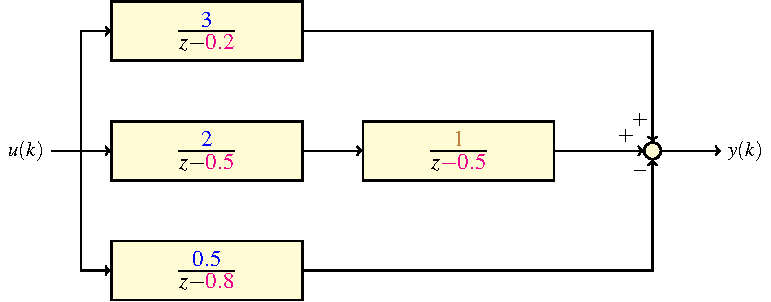
\includegraphics[width=0.85\columnwidth]{./Unit-03/img/PS01-ex04-fig01.pdf}
           \end{center}}
 \only<3 >{Take their outputs as state variables:\\%
           \begin{center}
            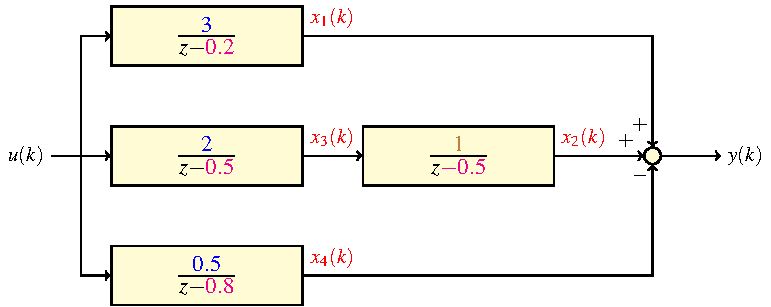
\includegraphics[width=0.85\columnwidth]{./Unit-03/img/PS01-ex04-fig02.pdf}
           \end{center}}
 \only<4->{write the elementary difference equations for each block:\\%
           \begin{center}
            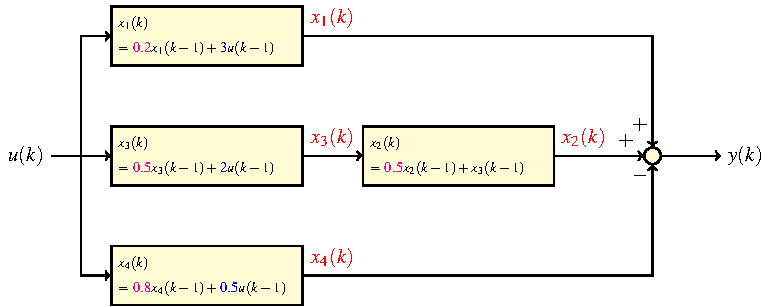
\includegraphics[width=0.85\columnwidth]{./Unit-03/img/PS01-ex04-fig03.pdf}
           \end{center}}
\end{frame}

\begin{frame}
\frametitleTC{Solution}
\framesubtitleTC{Item (b)}
\myPause
 \begin{itemize}[<+-| alert@+>]
 \item Now put it all together:
       \begin{displaymath}
        \left\{\begin{array}{rlllll}
         x_1(k) &= 0.2x_1(k-1) &              &              &              & +u(k-1)    \\
         x_2(k) &=             & +0.5x_2(k-1) & +x_3(k-1)                                \\
         x_3(k) &=             &              &  0.5x_3(k-1) &              & +2u(k-1)   \\
         x_4(k) &=             &              &              &  0.8x_4(k-1) & +0.5u(k-1) \\
         y(k)   &= x_1(k)      & +x_2(k)      &              & -x_4(k)                   \\
        \end{array}\right.
       \end{displaymath}
 \item Hence
       \begin{displaymath}
        \begin{array}{c}
         A = \begin{bmatrix}
              0.2 & 0   & 0   & 0   \\
              0   & 0.5 & 1   & 0   \\
              0   & 0   & 0.5 & 0   \\
              0   & 0   & 0   & 0.8
             \end{bmatrix}, \quad
         b = \begin{bmatrix} 1 \\ 0 \\ 2 \\ 0.5 \end{bmatrix}, \\ \\
         c = \begin{bmatrix} 1 & 0 & 1 & -1 \end{bmatrix}, \quad
         d = 0.
        \end{array}
       \end{displaymath}
 \end{itemize}
\end{frame}

\begin{frame}
\frametitleTC{Takeaways}
\framesubtitleTC{from exercise 04}
\myPause
 \begin{itemize}[<+-| alert@+>]
 \item We know that the poles of $G(z)$ are eigenvalues of $A$.
 \item Not THE eigenvalues, some may be cancelled.
 \item Our matrices are real, hence eigenvalues (and poles) are either real, or in complex
       conjugate couples. Here we limit the math to real ones (but results hold in general).
 \item \vfill It should be clear that \emph{any} $G(z)$, once decomposed in simple fractions,\\
       can be treated as we did.
 \item Can we say something on our $A$? Can we use it to understand\\
       the eigenvalues--stability relationship we mentioned? 
 \item Remember that the free motion of a system converges to zero,\\
       diverges or neither, if so  does $A^k$ for $k\rightarrow\infty$. Let us have a look\\
       with this idea in mind.
 \end{itemize}
\end{frame}

\begin{frame}
\frametitleTC{Takeaways}
\framesubtitleTC{from exercise 04}
\myPause
 \begin{itemize}[<+-| alert@+>]
 \item In general, once treated as we did, matrix $A$ looks e.g. as follows:
 \begin{displaymath}
  A = 
  \begin{bmatrix}
   \-& \cellcolor{green!30!white}{\lambda_{1}} & 0 & 0 & 0 & 0 & 0 & 0 & \ldots & \\
   \-& 0 &\cellcolor{green!30!white}{\lambda_{2}}  & 0 & 0 & 0 & 0 & 0 \\
   \-& 0 & 0 &\cellcolor{orange!50!white}{\lambda_{3}}
             &\cellcolor{yellow!30!white}{\textcolor{cyan!80!black}{0}} & 0 & 0 & 0 \\
   \-& 0 & 0 &\cellcolor{yellow!30!white}{0}
             &\cellcolor{orange!50!white}{\lambda_{3}} & 0 & 0 & 0 \\
   \-& 0 & 0 & 0 & 0 &\cellcolor{orange!50!white}{\lambda_{4}}
                     &\cellcolor{orange!30!white}{\textcolor{red}{1}} & \cellcolor{yellow!30!white}{0} \\
   \-& 0 & 0 & 0 & 0 &\cellcolor{orange!30!white}{0}
                     &\cellcolor{orange!50!white}{\lambda_{4}}
                     & \cellcolor{yellow!30!white}{\textcolor{cyan!80!black}{0}} \\
   \-& 0 & 0 & 0 & 0 &\cellcolor{yellow!30!white}{0}
                     &\cellcolor{yellow!30!white}{0} & \cellcolor{orange!50!white}{\lambda_{4}} \\
   \-& \vdots &&&&&&& \ddots \\
  \end{bmatrix}
 \end{displaymath}
 \item Notice the block diagonal structure:
       \begin{itemize}[<+-| alert@+>]
       \item \colorbox{green!30!white}{single} eigenvalues are just diagonal elements;
       \item \colorbox{orange!50!white}{multiple} ones are repeated to form square \colorbox{yellow!30!white}{blocks},
       \item in turn diagonally composed of \colorbox{orange!30!white}{mini-blocks} separated by
             \textcolor{cyan!80!black}{zeroes}\\
             that break the over-diagonal sequence of \textcolor{red}{ones} in the block.
       \end{itemize}
 \end{itemize}
\end{frame}

\begin{frame}
\frametitleTC{Takeaways}
\framesubtitleTC{from exercise 04}
\myPause
 \begin{itemize}[<+-| alert@+>]
 \item Now, let us compute $A^k$:\myPause
 \begin{displaymath}
  A^k = 
  \begin{bmatrix}
   \-& \cellcolor{green!30!white}{\lambda_{1}^k} & 0 & 0 & 0 & 0 & 0 & 0 & \ldots & \\
   \-& 0 &\cellcolor{green!30!white}{\lambda_{2}^k}  & 0 & 0 & 0 & 0 & 0 \\
   \-& 0 & 0 &\cellcolor{orange!50!white}{\lambda_{3}^k}
             &\cellcolor{yellow!30!white}{\textcolor{cyan!80!black}{0}} & 0 & 0 & 0 \\
   \-& 0 & 0 &\cellcolor{yellow!30!white}{0}
             &\cellcolor{orange!50!white}{\lambda_{3}^k} & 0 & 0 & 0 \\
   \-& 0 & 0 & 0 & 0 &\cellcolor{orange!50!white}{\lambda_{4}^k}
                     &\cellcolor{orange!30!white}{\textcolor{red}{k\lambda_4^{k-1}}} & \cellcolor{yellow!30!white}{0} \\
   \-& 0 & 0 & 0 & 0 &\cellcolor{orange!30!white}{0}
                     &\cellcolor{orange!50!white}{\lambda_{4}^k}
                     & \cellcolor{yellow!30!white}{\textcolor{cyan!80!black}{0}} \\
   \-& 0 & 0 & 0 & 0 &\cellcolor{yellow!30!white}{0}
                     &\cellcolor{yellow!30!white}{0} & \cellcolor{orange!50!white}{\lambda_{4}^k} \\
   \-& \vdots &&&&&&& \ddots \\
  \end{bmatrix}
 \end{displaymath}\myPause
 \item Does it converge to a matrix of zeroes? Or diverge --- i.e., does\\
       at least one element diverge? Or neither?
 \item In other words, is the system asymptotically stable, unstable,\\
       or (simply) stable?
 \end{itemize}
\end{frame}

\begin{frame}[fragile]
\frametitleTC{Takeaways}
\framesubtitleTC{from exercise 04}
\myPause
 \begin{itemize}[<+-| alert@+>]
 \item Diagonal terms, in the form $\lambda^k$:
       \begin{displaymath}
        \begin{array}{rcl}
         \lim\limits_{k\rightarrow\infty}|\lambda^k| = 
          \begin{cases}
           0        & |\lambda| < 1 \\
           1        & |\lambda| = 1 \\
           \infty   & |\lambda| > 1 \\
          \end{cases}
        \end{array}
       \end{displaymath}
 \item Over-diagonal terms, in the form $k\lambda^k$:
       \begin{displaymath}
        \begin{array}{rcl}
         \lim\limits_{k\rightarrow\infty}|k\lambda^k| = 
          \begin{cases}
           0        & |\lambda| < 1 \\
           \infty   & |\lambda| \geq 1 \\
          \end{cases}
        \end{array}
       \end{displaymath}
 \item NOTE: larger mini-blocks give over-diagonal terms in other forms,\\
       but analogous as for the above. Take wxMaxima and try e.g.\\
       {\small
       \begin{verbatim}
  A:matrix([lambda,1,0],[0,lambda,1],[0,0,lambda]);
  A.A.A; /* NOT A^3, that is the elem-by-elem power */
       \end{verbatim}
       }
 \end{itemize}
\end{frame}

\begin{frame}
\frametitleTC{Takeaways}
\framesubtitleTC{from exercise 04}
\myPause
 \begin{itemize}[<+-| alert@+>]
 \item Now let us put it all together:
       \begin{itemize}[<+-| alert@+>]
       \item each single eigenvalue $\lambda_i$ only gives one diagonal term $\lambda_i^k$;
       \item each eigenvalue $\lambda_j$ with multiplicity $n_j$ gives $n_j$ diagonal terms $\lambda_j^k$, plus some\\
             \vspace{-0.75mm}over-diagonal terms $k\lambda_j^k$ -- or analogous -- iff the maximum size of its mini-block\\
             is greater then one.
       \end{itemize}
 \item Hence\\
       {\scriptsize 
       %\begin{center}
        \begin{tabular}{rcl}
         all $|\lambda_i|<1$                             & $\Rightarrow$ & System asymptotically stable\\
         \\
         at least one $|\lambda_i|>1$                    & $\Rightarrow$ & System unstable\\
         \\
         all $|\lambda_i|\leq 1$                         & \\
         and at least one has unity magnitude            & $\Rightarrow$ & System (simply) stable\\
         but in this case also unity max mini-block size & \\
         \\
         otherwise (i.e.,all $|\lambda_i|\leq 1$, and    & \\
         at least one has both unity magnitude and       & $\Rightarrow$ & System unstable\\
         maximum mini-block size greater than one)       & \\
        \end{tabular}
       %\end{center}
       }
 \item \vfill This proves (and completes) the statement of slide~\ref{pag:stab-eivals}.
 \end{itemize}
\end{frame}

 


\section{Wrap-up}
\subsection{}

\begin{frame}
\frametitleTC{Ideas and capabilities to take home}
\framesubtitleTC{(1/2) not necessarily in the same order as we saw them...}
 \begin{itemize}[<+-| alert@+>]
 \item Interpreting the state space description of a DT LTI dynamic system\\
       as scalar equations.
 \item Computing a system's transfer function from its state space description.
 \item Computing state and output responses in the time domain, and distinguishing\\
       free and induced motion.
 \item Commonly used signals: impulse, step, ramp.
 \end{itemize}
\end{frame}

\begin{frame}
\frametitleTC{Ideas and capabilities to take home}
\framesubtitleTC{(2/2)}
 \begin{itemize}[<+-| alert@+>]
 \item Poles and zeroes of a transfer functions, the former being eigenvalues\\
       of the dynamic matrix.
 \item Pole/zero cancellations and hidden parts.
 \item Writing a dynamic system as block diagram and recognise the inherent\\
       feedback in it.
 \item Combining blocks into overall transfer functions: for the moment series and parallel, more
       on this subject later on.
 \item A possible way to transform a transfer function into a state space\\
       representation.
 \item Stability and eigenvalues of the dynamic matrix (for the curious,\\
       we proved our statement by writing that matrix in \TC{Jordan} form).
 \end{itemize}
\end{frame}



%%% UNIT 4
{
\setbeamertemplate{headline}{}
\setbeamertemplate{footline}{
  \begin{beamercolorbox}[wd=\paperwidth,ht=2.2ex,dp=1.5ex]{palette quaternary}
  \end{beamercolorbox}
  }
\begin{frame}[noframenumbering]
\frametitle{\DB{\huge{\textbf{$\blacksquare$ Unit 4}}}}
\myPause
 \begin{itemize}
 \item[] \LARGE{\MB{System responses}}
 \item[] \vspace{-1mm}\LARGE{\MB{Formalising requirements}}
 \item[] \vspace{-1mm}\LARGE{\MB{The control loop}}
 \item[] \vspace{-1mm}\LARGE{\MB{Direct synthesis -- PIDs appearing on the horizon...}}
 \item[] \vspace{-1mm}\LARGE{\MB{Conclusions and discussion}}
 \end{itemize}
\end{frame}
}

\part{}

\section{System responses}
\subsection{}

\begin{frame}\mccz
\frametitleTC{Foreword}
\framesubtitleTC{}
\myPause
 \begin{columns}
  \column[T]{0.35\textwidth}
   \only<2->{\centering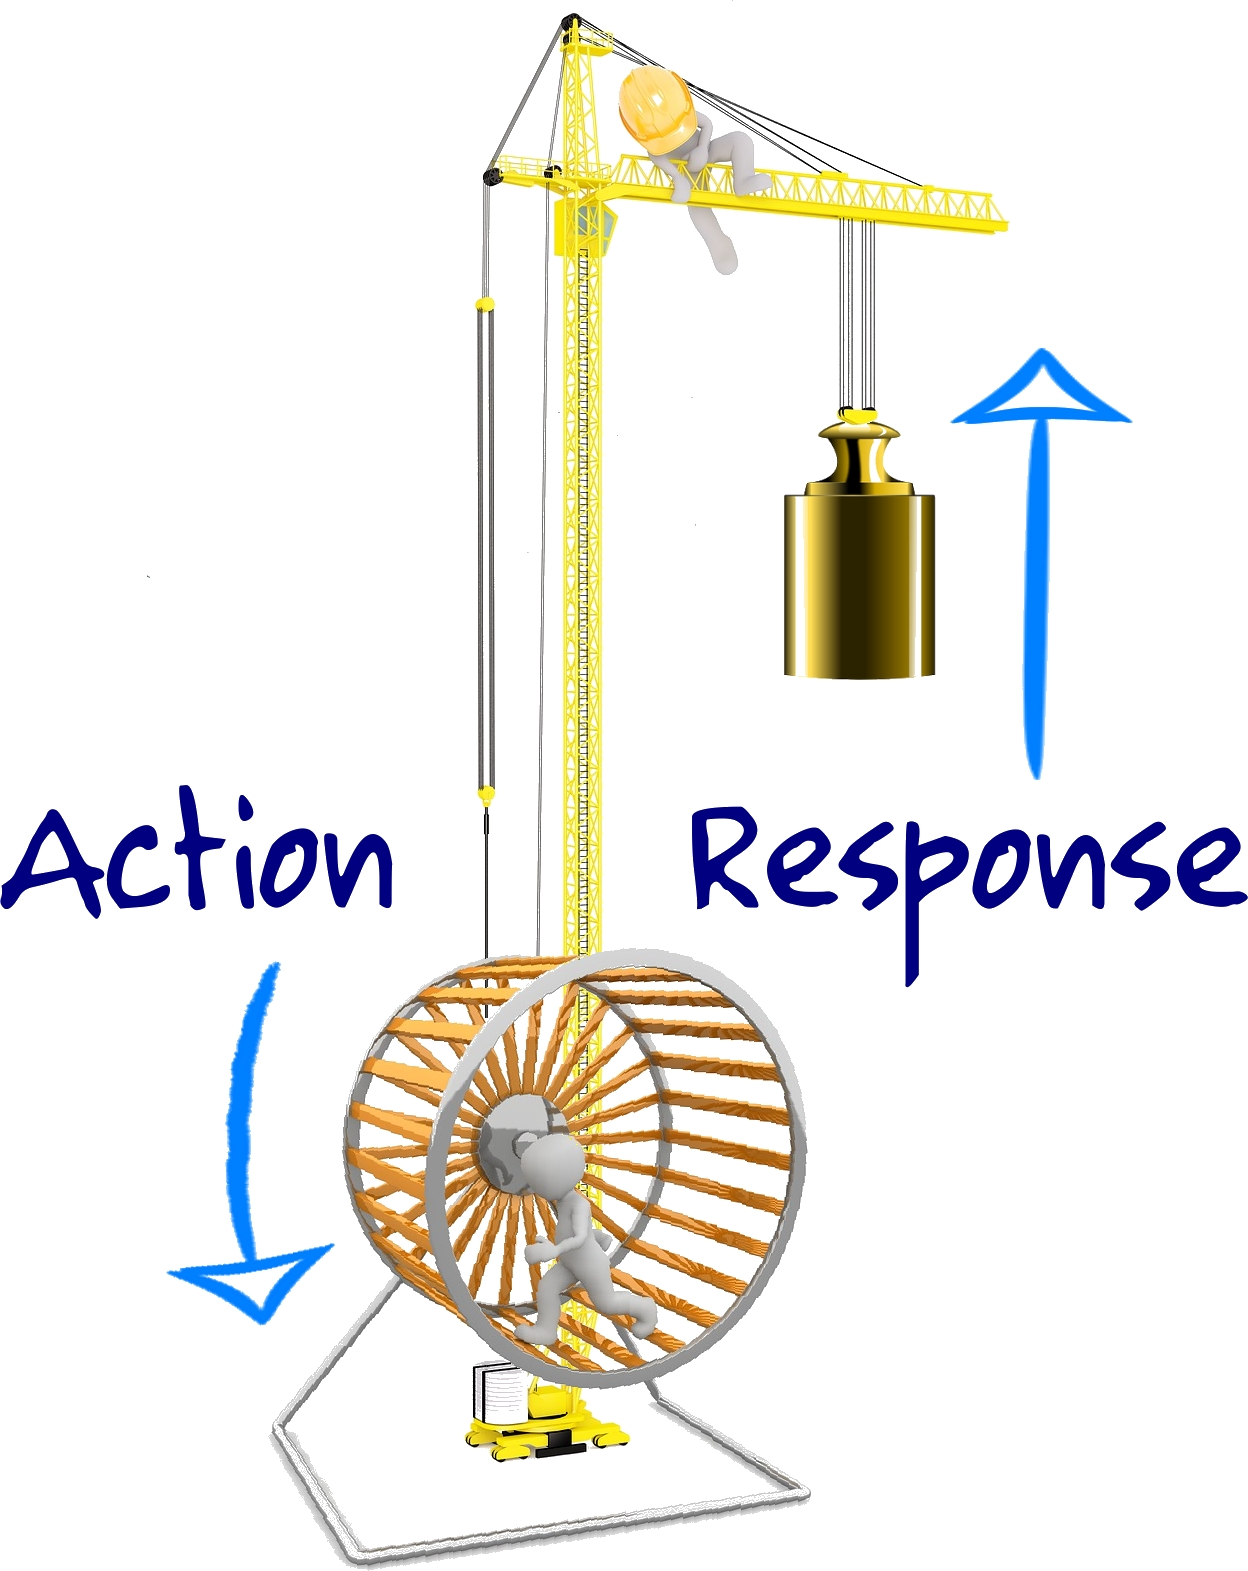
\includegraphics[height=6cm]{./Unit-04/img/response-intro_cc0.jpg}}\myPause%
  \column[T]{0.65\textwidth}
   \begin{itemize}[<+-| alert@+>]
   \item We know how to describe a (DT LTI) dynamic system
         \begin{itemize}[<+-| alert@+>]
         \item in the state space with $(A,b,c,d)$
         \item and with a transfer function $G(z)$.
         \end{itemize}
   \item But how do these descriptions relate to the way\\
         the system responds to a certain \emph{stimulus}?
   \item Specifically for our purpose, can we somehow\\
         relate a transfer function to its\\
         \TC{time (domain) responses}?
   \item \vspace{3mm} Of course we can.
   \item Let us see first how and then why.
   \end{itemize}
 \end{columns}
\end{frame}

\begin{frame}
\frametitleTC{Foreword}
\framesubtitleTC{An introductory case}
\myPause
 \begin{itemize}[<+-| alert@+>]
 \item We showed that as long as a system has only real eigenvalues, its transfer function can be
       expressed as sum/product of elementary first order terms in the form
       \begin{displaymath}
        g(z) = \frac{\mu}{z-p}
       \end{displaymath}
 \item NOTE: if all eigenvalues are distinct, a sum (no products) of terms\\
       like the above suffices.
 \item Given the linearity of the system, responses will sum together the\\
       same way as elementary terms in the transfer function do.
 \item We therefore start by analysing the responses of $g(z)$ above\\
       to a unit impulse and a unit step.
 \item We deal with TI systems, hence in the following everything starts\\
       at $k=0$.
 \end{itemize}
\end{frame}

\begin{frame}
\frametitleTC{An introductory case}
\framesubtitleTC{Impulse response of $g(z)$}
\myPause
 \begin{itemize}[<+-| alert@+>]
 \item Recalling the meaning of $z$, $g(z)$ in the time domain means
       \begin{displaymath}
        y(k) = p y(k-1) + \mu u(k-1).
       \end{displaymath}
 \item Set now $u(k)=imp(k)$, i.e., the sequence $\{1,0,0,0,\ldots\}$. We assume no action on the system
       before $k=0$, consistently with the definition of impulse. We also assume the system at rest, otherwise
       there is free motion and we don not see ONLY the response to $u$, hence $y=0$ for $k<0$.
 \item This said, we get
       {\small
       \begin{displaymath}
        \begin{array}{lclclclclcl}
         y(0) &=& p y(-1) + \mu u(-1) &=& p \cdot 0     + \mu \cdot 0 &=& 0       \\
         y(1) &=& p y(0)  + \mu u(0)  &=& p \cdot 0     + \mu \cdot 1 &=& \mu     \\
         y(2) &=& p y(1)  + \mu u(1)  &=& p \cdot \mu   + \mu \cdot 0 &=& \mu p   \\
         y(3) &=& p y(2)  + \mu u(2)  &=& p \cdot \mu p + \mu \cdot 0 &=& \mu p^2 \\
         \ldots
        \end{array}
       \end{displaymath}
       }
 \item \vspace{-4mm}i.e., the sequence $\{0,\mu,\mu p,\mu p^2,\mu p^3,\ldots\}$.
 \end{itemize}
\end{frame}

\begin{frame}[fragile]
\frametitleTC{An introductory case}
\framesubtitleTC{Impulse response of $g(z)$}
\myPause
 \begin{itemize}[<+-| alert@+>]
 \item Summarising, the impulse response of $g(z)$ is
       \begin{displaymath}
        y(k) = \begin{cases}
                0           & k=0 \\
                \mu p^{k-1} & k>0
               \end{cases}
       \end{displaymath}
 \item Let us compute and plot this response with Scilab:
       {\small
       \begin{verbatim}
 g   = syslin('d',1/(%z-0.5)); // define transfer function ('d' means DT)
 gss = tf2ss(g);               // convert to state space for dsimul
 u   = [1,0,0,0,0,0,0,0,0,0];  // impulse sequence (10 samples)
 y   = dsimul(gss,u);          // compute response
 plot(y,'.');                  // plot (as dots)
       \end{verbatim}
       }
 \item Try different values of $\mu$ and $p$, and comment on the results.
 \end{itemize}
\end{frame}

\begin{frame}
\frametitleTC{An introductory case}
\framesubtitleTC{Impulse response of $g(z)$ -- general remarks}
\myPause
 \begin{itemize}[<+-| alert@+>]
 \item The pole $p$ governs stability as we already know.
 \item For $p=0$ the system is a pure one-step delay.
 \item For $0<p<1$ the response converges monotonically, for $-1<p<0$ oscillating.
 \item In both cases, $p$ governs the convergence speed.
 \item For $p=1$ the response is constant, for $p=-1$ a sustained oscillation\\
       (in both cases for $k>0$, obviously).
 \item Parameter $\mu$ acts as a (signed) scale factor.
 \end{itemize}
\end{frame}

\begin{frame}
\frametitleTC{An introductory case}
\framesubtitleTC{Step response of $g(z)$}
\myPause
 \begin{itemize}[<+-| alert@+>]
 \item Set $u(k)=step(k)$, i.e., the sequence $\{1,1,1,1,\ldots\}$.
 \item We can verify that this yields the response
       \begin{displaymath}
        y(k) = \frac{\mu}{1-p}(1-p^k)
       \end{displaymath}
 \item To this end, we observe that with $\mu=1-p$ we get $y(k) = 1-p^k$:
       {\scriptsize
       \begin{displaymath}
        \begin{array}{lclclclclcl}
         y(0) &=& p \cdot 0       + (1-p) \cdot 0 & &           &=& 0     \\
         y(1) &=& p \cdot 0       + (1-p) \cdot 1 & &           &=& 1-p   \\
         y(2) &=& p \cdot (1-p)   + (1-p) \cdot 1 &=& p-p^2+1-p &=& 1-p^2 \\
         y(3) &=& p \cdot (1-p^2) + (1-p) \cdot 1 &=& p-p^3+1-p &=& 1-p^3 \\
         y(4) &=& p \cdot (1-p^3) + (1-p) \cdot 1 &=& p-p^4+1-p &=& 1-p^4 \\
         y(5) &=& p \cdot (1-p^4) + (1-p) \cdot 1 &=& p-p^5+1-p &=& 1-p^5 \\
         \ldots
        \end{array}
       \end{displaymath}
       }
 \item \vspace{-4mm}Hence a generic $\mu$ scales $y$ to give the result above.
 \end{itemize}
\end{frame}

\begin{frame}[fragile]
\frametitleTC{An introductory case}
\framesubtitleTC{Step response of $g(z)$}
\myPause
 \begin{itemize}[<+-| alert@+>]

 \item Also for the step response case, let us compute and plot some examples with Scilab:
       {\small
       \begin{verbatim}
 g   = syslin('d',1/(%z-0.5)); // define transfer function ('d' means DT)
 gss = tf2ss(g);               // convert to state space for dsimul
 u   = ones(1,10)              // step sequence (a row of 10 samples)
 y   = dsimul(gss,u);          // compute response
 plot(y,'.');                  // plot (as dots)
       \end{verbatim}
       }
 \item Try again different values of $\mu$ and $p$, and comment on the results.
 \end{itemize}
\end{frame}

\begin{frame}
\frametitleTC{An introductory case}
\framesubtitleTC{Step response of $g(z)$ -- general remarks}
\myPause
 \begin{itemize}[<+-| alert@+>]
 \item The pole $p$ governs stability as we already know.
 \item For $p=0$ the system is a pure one-step delay.
 \item For $0<p<1$ the response converges monotonically, for $-1<p<0$ oscillating.
 \item In both cases, $p$ governs the convergence speed.
 \item For $p=1$ the response is a diverging ramp, for $p=-1$ a sustained oscillation.
 \item If $y(k)$ converges, it does so to the value
       \begin{displaymath}
        \frac{\mu}{1-p} = g(1)
       \end{displaymath}
       that is called the \TC{gain} of the transfer function.
 \item Hence for an asymptotically stable $g(z)$, if for $k\rightarrow\infty$ $u(k)\rightarrow\overline{u}$,\\
       then $y(k)\rightarrow g(1)\overline{u}$.
 \end{itemize}
\end{frame}

\begin{frame}
\frametitleTC{Generalisation}
\framesubtitleTC{}
\myPause
 \begin{itemize}[<+-| alert@+>]
 \item In the same way we treated the elementary term $g(z)$, we could address a generic transfer function.
 \item However
       \begin{itemize}[<+-| alert@+>]
       \item as long as there are single poles (eigenvalues), the response will be a linear 
             combination of terms like those yielded by $g(z)$,
       \item while multiple eigenvalues (poles) can be treated like we did from slide~\ref{pag:ex-realisation}
             onward (enough on this for our purposes),
       \item and complex poles could be a nice exercise for the interested \smiley\\
             although here we do not address them either.
       \end{itemize}
 \item We do not treat the most general case, nonetheless we go through\\
       one non-elementary example as this allows for useful considerations.
 \end{itemize}
\end{frame}

\begin{frame}
\frametitleTC{Generalisation}
\framesubtitleTC{One model class, some particular cases}
\myPause
 \begin{itemize}[<+-| alert@+>]
 \item Take the class of transfer functions with up to two poles and one zero
       \begin{displaymath}
        G(z) = \frac{b_0+b_1z}{a_0+a_1z+a_2z^2}
       \end{displaymath}
 \item and specialise it to the four cases
       \begin{displaymath}
        \begin{array}{c}
         G_A(z) = \cfrac{1}{z}, \qquad
         G_B(z) = \cfrac{0.5}{z-0.5}, \qquad
         G_C(z) = \cfrac{(1-0.25)^2}{1-0.55} \, \cfrac{z-0.55}{(z-0.25)^2}, \\ \\
         G_D(z) = \cfrac{2.5-1}{(1-0.5)^2} \, \cfrac{2.5-z}{(z-0.5)^2}.
        \end{array}
       \end{displaymath}
 \item Notice that for clarity in the following plots they all have unity\\
       gain, i.e., $G_{A,B,C,D}(1)=1$.
 \end{itemize}
\end{frame}

\begin{frame}
\frametitleTC{Generalisation}
\framesubtitleTC{One model class, different responses}
\myPause
 \begin{itemize}[<+-| alert@+>]
 \item The corresponding four (unit) step responses are plotted below with the so-called\\
       ``staircase'' style:
       \begin{center}
        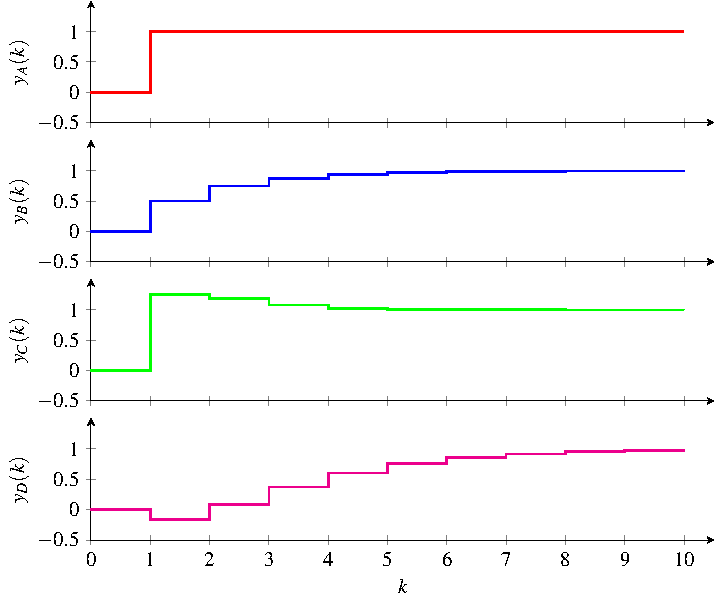
\includegraphics[width=0.50\columnwidth]{./Unit-04/img/StepRespTypes.pdf}
       \end{center}
 \item \vspace{-3mm} Let us try to provide some possible interpretation.
 \end{itemize}
\end{frame}

\begin{frame}
\frametitleTC{Generalisation}
\framesubtitleTC{One model class, different responses}
\myPause
 \begin{columns}
  \column[T]{0.45\textwidth}
   \only<2->{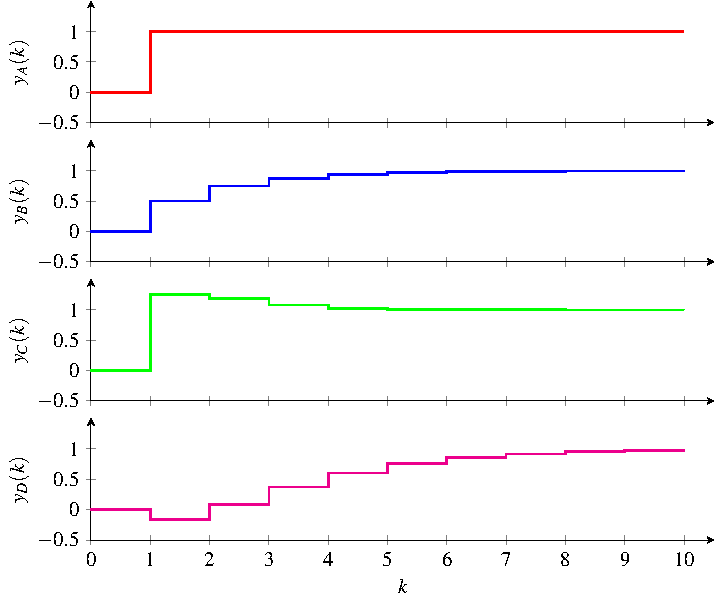
\includegraphics[height=5.5cm]{./Unit-04/img/StepRespTypes.pdf}}
  \column[T]{0.55\textwidth}
   \begin{itemize}[<+-| alert@+>]
   \item Suppose $u(k)$ and $y(k)$ to be respectively a resource to allot and its effect.
         \begin{itemize}[<+-| alert@+>]
         \item[A.] The resource is acquired and exerts immediately its effect (that is therefore
                   seen at the very next step).
         \item[B.] The resource acts immediately but takes some steps to yield its full effect\\
                   (for example because first\\
                   some queue needs\\
                   emptying).
         \end{itemize}
   \end{itemize}
 \end{columns}
\end{frame}

\begin{frame}
\frametitleTC{Generalisation}
\framesubtitleTC{One model class, different responses}
 \begin{columns}
  \column[T]{0.45\textwidth}
   \only<1->{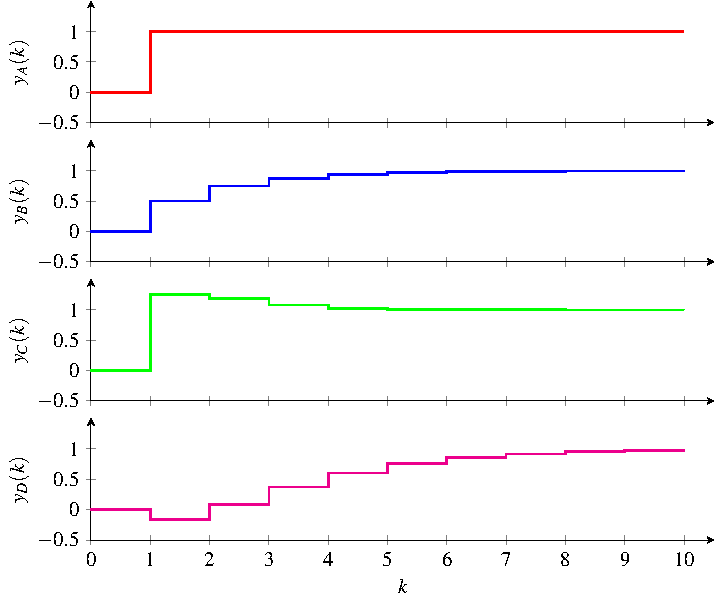
\includegraphics[height=5.5cm]{./Unit-04/img/StepRespTypes.pdf}}
  \column[T]{0.55\textwidth}
   \begin{itemize}[<+-| alert@+>]
   \item Suppose $u(k)$ and $y(k)$ to be respectively a resource to allot and its effect.
         \begin{itemize}[<+-| alert@+>]
         \item[C.] The resource produces a transiently enhanced effect (this is quite typical
                   when the resource is computational power and the effect is the \emph{speed} toward a goal).
         \item[D.] The resource requires some effort to be acquired and initially \emph{reduces}
                   performance, like a new\\
                   core that when acquired\\
                   has an unknown cache\\
                   content, thus causing\\
                   a lot of cache misses.
         \end{itemize}
   \end{itemize}
 \end{columns}
\end{frame}

\begin{frame}
\frametitleTC{Generalisation}
\framesubtitleTC{Lessons learnt and next steps}
\myPause
 \begin{itemize}[<+-| alert@+>]
 \item One model can produce very different responses \TC{by just changing parameters}, thus fitting
       several physical cases --- remember the remark in the introductory section, that we need a systems
       and control theory because determining a controller is largely physics-independent?.
 \item \vspace{3mm} We shall now see how control requirements can be stipulated by saying that some response
       to some \emph{stimulus} should have a certain aspect.
 \item We shall then convert this into requiring some \TC{transfer function}\\
       to have a certain aspect...
 \item ...and finally start synthesising feedback controllers.
 \end{itemize}
\end{frame}


\section{Formalising requirements}
\subsection{}

\begin{frame}
\frametitleTC{A time-domain viewpoint}
\framesubtitleTC{}
\myPause
 \begin{itemize}[<+-| alert@+>]
 \item Requirements are expressed in the time domain very naturally.
 \item Suppose to apply a step variation to the set point $w(k)$, and consider four possible\\
       responses of the controlled variable $y(k)$ --- points are joined with segments\\
       to improve readability:
       \begin{center}
        \vspace{2mm}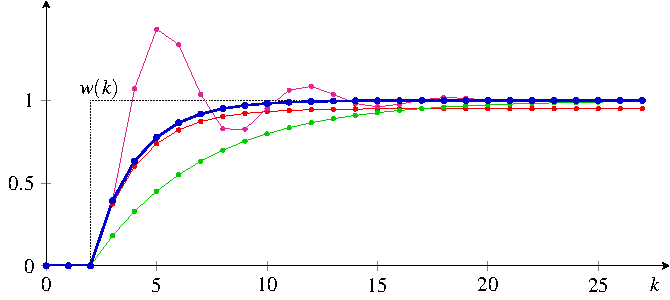
\includegraphics[width=0.60\columnwidth]{./Unit-04/img/StepRespForRequirements.pdf}
       \end{center}
 \end{itemize}
\end{frame}

\begin{frame}
\frametitleTC{A time-domain viewpoint}
\framesubtitleTC{}
\myPause
 \begin{center}
  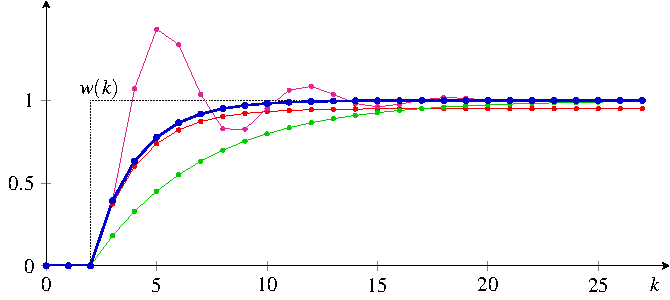
\includegraphics[width=0.40\columnwidth]{./Unit-04/img/StepRespForRequirements.pdf}
 \end{center}\myPause
 \begin{itemize}[<+-| alert@+>]
 \item The ``control quality'' (for the moment, in the most intuitive sense)\\
       is different:
       \begin{itemize}[<+-| alert@+>]
       \item \textcolor{blue!80!black}{blue} -- good;
       \item \textcolor{red!95!black}{red} -- does not reach the new desired value exactly;
       \item \textcolor{green!80!black}{green} -- too slow;
       \item \textcolor{magenta!95!black}{magenta} -- oscillatory.
       \end{itemize}
 \end{itemize}
\end{frame}

\begin{frame}
\frametitleTC{A time-domain viewpoint}
\framesubtitleTC{}
\myPause
 \begin{itemize}[<+-| alert@+>]
 \item Indeed, many requirements are straightforwardly expressed by stating e.g. how the response
       of the controlled variable to a certain variation of the set point has to look.
 \item For example, one may require that
       \begin{itemize}[<+-| alert@+>]
       \item[] when $w(k)$ undergoes a step variation
       \item[] $y(k)$ has to enter a $\mp$5\% band around it in maximum 5 steps
       \item[] and then never exit that band,
       \item[] also never reaching a value more than 10\% above the new set point,
       \item[] and with a one-step variation not greater than half of the total one,
       \end{itemize}
 \item[] or express analogous desires.
 \end{itemize}
\end{frame}

\begin{frame}
\frametitleTC{A time-domain viewpoint}
\framesubtitleTC{}
\myPause
 \begin{itemize}[<+-| alert@+>]
 \item A quite articulated example to illustrate the idea is shown below: the response has to lie
       entirely within the evidenced area.
       \begin{center}
        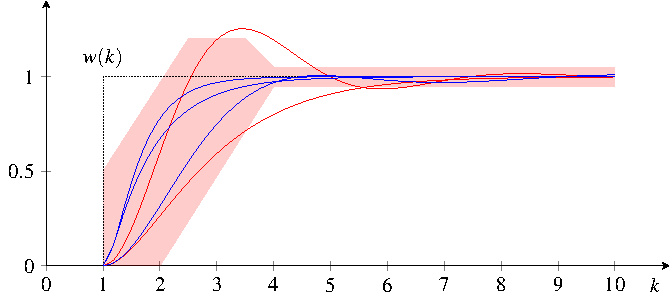
\includegraphics[width=0.60\columnwidth]{./Unit-04/img/StepRespWithConstraints-SP.pdf}
       \end{center}
 \item Blue responses are acceptable, red ones are not.
 \end{itemize}
\end{frame}


\begin{frame}
\frametitleTC{A time-domain viewpoint}
\framesubtitleTC{}
\myPause
 \begin{itemize}[<+-| alert@+>]
 \item The key idea we are soon introducing is that prescribing a certain aspect for the response
       of $y(k)$ to $w(k)$, in fact means prescribing characteristics of the transfer function
       from the former to the latter (as already anticipated).
 \item The same idea can be applied to the responses of $y(k)$ to disturbances, if the issue is to
       reject them.
 \item \vspace{3mm}This is not the only way to set requirements, but here we stick to this one.
 \item In the following we shall see how the idea above leads to synthesising\\
       a suitable controller --- and the PID structure will come into play\\
       \TC{with consciousness of the reasons for its wide applicability}.
 \item \vfill But prior to this, also to understand what a reasonable ``desired $y/w$\\
       transfer function'' can look like, we need to analyse the control loop\\
       formally.
 \end{itemize}
\end{frame}

\section{The control loop}
\subsection{}

\begin{frame}
\frametitleTC{The control loop and its actors}
\framesubtitleTC{}
\myPause
 \begin{itemize}[<+-| alert@+>]
 \item General representation:
       \begin{center}
        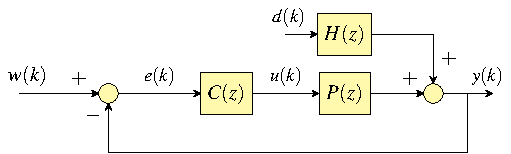
\includegraphics[width=0.50\columnwidth]{./Unit-04/img/ControlLoop.pdf}
       \end{center}
 \item Notation:
       \begin{itemize}[<+-| alert@+>]
       \item $w(k)$ is the \TC{set point} or \TC{reference};
       \item $y(k)$ is the \TC{controlled variable};
       \item $e(k)$ is the \TC{error};
       \item $u(k)$ is the \TC{control signal};
       \item $d(k)$ is a \TC{disturbance};
       \item $P(z)$ and $H(z)$ compose the \TC{controlled system} model;
       \item $C(z)$ is the \TC{controller} transfer function.
       \end{itemize}
 \end{itemize}
\end{frame}

\begin{frame}
\frametitleTC{The control loop and its actors}
\framesubtitleTC{}
 \begin{center}
  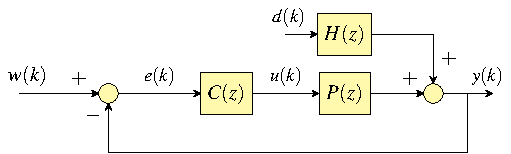
\includegraphics[width=0.40\columnwidth]{./Unit-04/img/ControlLoop.pdf}
 \end{center}
 \begin{itemize}[<+-| alert@+>]
 \item \vspace{-2mm} Some remarks:
       \begin{itemize}[<+-| alert@+>]
       \item we assume that the \TC{measurement} of $y$ reaching the node that generates the error,
             is exact (no disturbance on the feedback line) and instantaneous (no dynamic block
             on that line either);
       \item this may be \emph{very} questionable when some sensor is in the \emph{arena}, thus for\\
             example is not always assumed in process control, robotics and the like;
       \item however in computers most measurements are in fact the measured\\
             quantity itself (e.g., the one timer firing preemption interrupts and\\
             accounting CPU usage);
       \item this is an important simplification to exploit when applying control\\
             to computing system,
       \item with the exception of more ``physical'' controls (temperature, power,...)\\
             where sensor dynamics may be of some concern.
       \end{itemize}
 \end{itemize}
\end{frame}

\begin{frame}
\frametitleTC{Intermezzo}
\framesubtitleTC{Composing blocks in a feedback structure (we still miss this besides series and parallel)}
 \begin{center}
  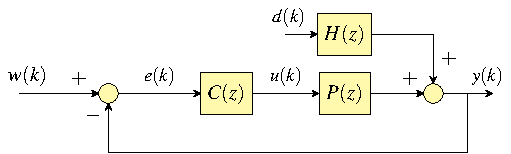
\includegraphics[width=0.40\columnwidth]{./Unit-04/img/ControlLoop.pdf}
 \end{center}\myPause
 \begin{itemize}[<+-| alert@+>]
 \item We need to compute the transfer functions from $w$ and $d$ to $y$ and $u$.
 \item To this end, imagine to cut the loop (for example right of the node summing the outputs of $P$ and $H$).
 \item Equating the left and the right side of this fictitious cut we have
       \begin{displaymath}
        H(z)d(k) + P(z)C(z) \left(w(k)-y(k) \right) = y(k),
       \end{displaymath}
 \item whence rearranging
       \begin{displaymath}
        y(k) = \frac{P(z)C(z)}{1+P(z)C(z)} w(k) + \frac{H(z)}{1+P(z)C(z)} d(k).
       \end{displaymath}
 \end{itemize}
\end{frame}

\begin{frame}
\frametitleTC{Intermezzo}
\framesubtitleTC{Composing blocks in a feedback structure}
\myPause
 \begin{itemize}[<+-| alert@+>]
 \item We adopt from now on the convention of calling $G_{ba}(z)$ the transfer function from $a(k)$ to $b(k)$
       when convenient --- btw, mind the subscript order. 
 \item We also recall the operatorial meaning of a transfer function, and that it represents the \TC{effect}
       of a certain input to a certain output. In other words, in our case we should for completeness write
       \begin{displaymath}
        G_{yw}(z) = \left. \frac{y(k)}{w(k)} \right|_{d(k)=0}, \qquad
        G_{yd}(z) = \left. \frac{y(k)}{d(k)} \right|_{w(k)=0},
       \end{displaymath}
       but we drop part of the notation for simplicity.
 \item Summing up, we have
       \begin{displaymath}
        G_{yw}(z) = \frac{P(z)C(z)}{1+P(z)C(z)}, \qquad
        G_{yd}(z) = \frac{H(z)}{1+P(z)C(z)}.
       \end{displaymath}
 \end{itemize}
\end{frame}

\begin{frame}
\frametitleTC{Intermezzo}
\framesubtitleTC{Composing blocks in a feedback structure}
\myPause
 \begin{center}
  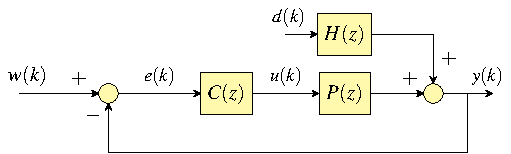
\includegraphics[width=0.40\columnwidth]{./Unit-04/img/ControlLoop.pdf}
 \end{center}\myPause
 \begin{itemize}[<+-| alert@+>]
 \item Reasoning in the same way for the output $u(k)$ -- details left as an exercise -- we have
       \begin{displaymath}
        G_{uw}(z) =  \frac{C(z)}{1+P(z)C(z)}, \qquad
        G_{ud}(z) = -\frac{C(z)H(z)}{1+P(z)C(z)}.
       \end{displaymath}
 \end{itemize}
\end{frame}

\begin{frame}
\frametitleTC{The control loop and its actors}
\framesubtitleTC{Main transfer functions of interest}
\myPause
 \begin{itemize}[<+-| alert@+>]
 \item Loop:
       \begin{displaymath}
        L(z) := P(z)C(z).
       \end{displaymath}
 \item From set point to controlled variable and control signal:
       \begin{displaymath}
        G_{yw}(z) = \frac{L(z)}{1+L(z)}, \qquad
        G_{uw}(z) = \frac{C(z)}{1+L(z)}.
       \end{displaymath}
 \item From disturbance to controlled variable and control signal:
       \begin{displaymath}
        G_{yd}(z) =  \frac{H(z)}{1+L(z)}, \qquad
        G_{ud}(z) = -\frac{C(z)H(z)}{1+L(z)}.
       \end{displaymath}
 \end{itemize}
\end{frame}

\begin{frame}
\frametitleTC{The control part of the loop}
\framesubtitleTC{Functional view}
\myPause
 \begin{itemize}[<+-| alert@+>]
 \item For the loop to operate
       \begin{itemize}[<+-| alert@+>]
       \item an \TC{event generator} triggers a new control action (periodically or on demand,\\
             here we stick to the former case);
       \item a \TC{sensor} is activated to get $y(k)$;
       \item the \TC{controller} $C(z)$ is invoked, and evolves as dynamic system by one step,
             \begin{itemize}[<+-| alert@+>]
             \item updating its state
             \item and then computing the new control $u(k)$;
             \end{itemize}
       \item an \TC{actuator} is activated to act on the process;
       \item and finally the system waits for a new event.
       \end{itemize}
 \item \vfill This view is quite easily related to CS frameworks such as\\
       the MAPE(-K).
 \item However, to design the controller, another view is preferable.
 \end{itemize}
\end{frame}

\begin{frame}
\frametitleTC{The control part of the loop}
\framesubtitleTC{Systemic view}
\myPause
 \begin{itemize}[<+-| alert@+>]
 \item For the loop to operate correctly
       \begin{itemize}[<+-| alert@+>]
       \item the closed-loop system must be asymptotically stable (more detail on this matter coming soon);
       \item the reference-to-output transfer function $G_{yw}(z)$, and/or the disturbance-to-output one $G_{yd}(z)$,
             must yield ``acceptable'' time responses in the presence of \TC{expectable} signals $w(k)$ and $d(k)$;
       \item the controller must be \TC{realisable}, i.e., the order of the numerator of $C(z)$ cannot exceed
             that of the denominator;
       \item in the opposite case, to explain the term ``realisable'', the controller\\
             output would depend on FUTURE samples of its input, which clearly\\ 
             is impossible to realise.
       \item We already saw that the above degree relationship is a structural\\
             property of any properly defined transfer function, incidentally.
       \end{itemize}
 \end{itemize}
\end{frame}

\begin{frame}\mccz
\frametitleTC{Time to start assembling our puzzle}
\framesubtitleTC{}
\myPause
 \begin{columns}
  \column[T]{0.35\textwidth}
   \only<2->{\includegraphics[height=6cm]{./Unit-04/img/PIDsOnTheHorizon_cc0.jpg}}
  \column[T]{0.65\textwidth}
   \begin{itemize}[<+-| alert@+>]
   \item First we shall learn a feedback control synthesis\\
         technique named ``direct'',
   \item then we shall discuss the relationships between\\
         the dynamic structure of the process\\
         and that of the controller,
   \item finally coming, as a quite natural\\
         consequence, to anticipate\\
         the PID control law. 
   \end{itemize}
 \end{columns}
\end{frame}



\section{Direct synthesis}
\subsection{}

\begin{frame}
\frametitleTC{Introductory example}
\framesubtitleTC{as usual...}
\myPause
 \begin{itemize}[<+-| alert@+>]
 \item Consider the control loop we know, with $H(z)=1$ for simplicity:
       \begin{center}
        \includegraphics[width=0.50\columnwidth]{./Unit-04/img/ControlLoop-H1.pdf}
       \end{center}
 \item Take as process and controller, respectively,
       \begin{displaymath}
        P(z) = \frac{\mu}{z-p}, \qquad
        C(z) = \frac{1-\alpha}{\mu} \, \frac{z-p}{z-1},
       \end{displaymath}
 \item and analyse the obtained system.
 \end{itemize}
\end{frame}

\begin{frame}
\frametitleTC{Introductory example}
\framesubtitleTC{}
\myPause
 \begin{itemize}[<+-| alert@+>]
 \item We have a \TC{zero/pole cancellation} between controller and process, as the loop transfer function is
       \begin{displaymath}
        L(z) = P(z)C(z)
             = \frac{\cbcancel[gray]{\mu}}{\ccancel[red]{z-p}} \,
               \frac{1-\alpha}{\cbcancel[gray]{\mu}} \, \frac{\ccancel[red]{z-p}}{z-1}
             = \frac{1-\alpha}{z-1}
       \end{displaymath}
 \item Hence
       \begin{displaymath}
        G_{yw}(z) = \frac{L(z)}{1+L(z)}
                  = \frac{\frac{1-\alpha}{z-1}}{1+\frac{1-\alpha}{z-1}}
                  = \frac{1-\alpha}{\ccancel[green!80!black]{z-1}} \,
                    \frac{\ccancel[green!80!black]{z-1}}{z-1+1-\alpha}
                  = \frac{1-\alpha}{z-\alpha}.
       \end{displaymath}
 \item NOTE: the \textcolor{green!80!black}{simplification} in computing $G_{yw}$ is NOT a cancellation.
 \item[] \vspace{-0.75mm}To have a cancellation you need a system (block) with a zero say\\
       in $\overline{z}$, and \TC{\underline{ANOTHER}} system (block) with a pole in the same  $\overline{z}$\\
 \item[] \vspace{-0.75mm} --- as is the case with the \textcolor{red}{cancellation} in $L$ above.
 \end{itemize}
\end{frame}

\begin{frame}
\frametitleTC{Introductory example}
\framesubtitleTC{}
\myPause
 \begin{itemize}[<+-| alert@+>]
 \item Furthermore, as $H(z)=1$,
       \begin{displaymath}
        G_{yd}(z) = \frac{1}{1+L(z)}
                  = \frac{1}{1+\frac{1-\alpha}{z-1}}
                  = \frac{z-1}{z-1+1-\alpha}
                  = \frac{z-1}{z-\alpha}.
       \end{displaymath}
 \item You may -- should \smiley$\,$ -- remember that cancellations entail hidden parts for the affected system.
 \item Let us evidence and discuss the implications of this in the present\\
       case, by going through a state space analysis.
 \end{itemize}
\end{frame}

\begin{frame}
\frametitleTC{Introductory example}
\framesubtitleTC{State space formulation of the closed-loop system}
\myPause
 \begin{itemize}[<+-| alert@+>]
 \item First we express the process in state space form:
       \begin{displaymath}
        \left\{\begin{array}{rcl}
         x_P(k) &=& p x_P(k-1) + \mu u(k-1) \\
         y(k)   &=& x_P(k) + d(k)
        \end{array}\right.
       \end{displaymath}
 \item Then we rewrite the controller transfer function as a constant plus a term with numerator degree
       strictly less than denominator degree (check out the wxMaxima \texttt{divide} function):
       \begin{displaymath}
        C(z) = \frac{1-\alpha}{\mu} \, \frac{z-p}{z-1} 
             = \frac{1-\alpha}{\mu} \left( 1 + \textcolor{red}{\frac{1-p}{z-1}} \right)
       \end{displaymath}
 \item Then we treat the \textcolor{red}{strictly proper} term like $P(z)$ above, obtaining
       \begin{displaymath}
        \left\{\begin{array}{rcl}
         x_C(k) &=& x_C(k-1) + (1-p) e(k-1) \\
         u(k)   &=& \frac{1-\alpha}{\mu} x_C(k) + \frac{1-\alpha}{\mu} e(k)
        \end{array}\right.
       \end{displaymath}
 \end{itemize}
\end{frame}

\begin{frame}
\frametitleTC{Introductory example}
\framesubtitleTC{State space formulation of the closed-loop system}
\myPause
 \begin{itemize}[<+-| alert@+>]
 \item Joining the equations for $P$ and $C$ and those for the node that produces $e$, gives\\
       for the overall closed-loop system the scalar (not yet reduced to minimal) description
       \begin{displaymath}
        \left\{\begin{array}{rcl}
         x_P(k) &=& p x_P(k-1) + \mu u(k-1) \\
         x_C(k) &=& x_C(k-1) + (1-p) e(k-1) \\
         y(k)   &=& x_P(k) + d(k) \\
         u(k)   &=& \frac{1-\alpha}{\mu} x_C(k) + \frac{1-\alpha}{\mu} e(k) \\
         e(k)   &=& w(k) - y(k)
        \end{array}\right.
       \end{displaymath}
 \end{itemize}
\end{frame}

\begin{frame}
\frametitleTC{Introductory example}
\framesubtitleTC{State space formulation of the closed-loop system}
\myPause
 \begin{itemize}[<+-| alert@+>]
 \item For the process state we have
       \begin{displaymath}
        \begin{array}{rcl}
         x_P(k) &=& p x_P(k-1) + \mu u(k-1) \\
                &=& p x_P(k-1) + \mu \left( \frac{1-\alpha}{\mu} x_C(k-1) + \frac{1-\alpha}{\mu} e(k-1) \right) \\
                &=& p x_P(k-1) + (1-\alpha)x_C(k-1) + (1-\alpha) \left( w(k-1)-y(k-1) \right) \\
                &=& p x_P(k-1) + (1-\alpha)x_C(k-1) + (1-\alpha) w(k-1)\\
                & & - (1-\alpha) \left( x_P(k-1)+d(k-1) \right) \\
                &=& \left( p+\alpha-1 \right) x_P(k-1)
                    +(1-\alpha) x_C(k-1)\\
                & & +(1-\alpha) w(k-1)
                    -(1-\alpha) d(k-1)                 
        \end{array}
       \end{displaymath}
 \item while the controller state evolves according to
       \begin{displaymath}
        \begin{array}{rcl}
         x_C(k) &=& x_C(k-1) + (1-p) e(k-1) \\
                &=& x_C(k-1)\\
                & & + (1-p) \left( w(k-1)-x_P(k-1)-d(k-1) \right)\\
                &=& (p-1) x_P(k-1) + x_C(k-1)\\
                & & +(1-p) w(k-1)
                    -(1-p) d(k-1)  
        \end{array}
       \end{displaymath}
 \end{itemize}
\end{frame}

\begin{frame}
\frametitleTC{Introductory example}
\framesubtitleTC{State space formulation of the closed-loop system}
\myPause
 \begin{itemize}[<+-| alert@+>]
 \item Putting it all together, the closed-loop system in state space form reads
       \begin{displaymath}
        \left\{\begin{array}{rcl}
         \begin{bmatrix} x_P(k) \\ x_C(k) \end{bmatrix}
         &=& 
         \begin{bmatrix} p+\alpha-1 & 1-\alpha \\ p-1 & 1  \end{bmatrix}
         \begin{bmatrix} x_P(k-1) \\ x_C(k-1) \end{bmatrix}
         +
         \begin{bmatrix} 1-\alpha & \alpha-1 \\ 1-p & p-1  \end{bmatrix}
         \begin{bmatrix} w(k-1) \\ d(k-1) \end{bmatrix} \\
         \begin{bmatrix} y(k) \\ u(k) \end{bmatrix}
         &=& 
         \begin{bmatrix} 1 & 0 \\ \frac{\alpha-1}{\mu} & \frac{1-\alpha}{\mu} \end{bmatrix}
         \begin{bmatrix} x_P(k) \\ x_C(k) \end{bmatrix}
         +
         \begin{bmatrix} 0 & 1 \\ \frac{1-\alpha}{\mu} & \frac{\alpha-1}{\mu} \end{bmatrix}
         \begin{bmatrix} w(k) \\ d(k) \end{bmatrix} \\
        \end{array}\right.
       \end{displaymath}
 \item[] with input $[w\,d]'$, output $[y\,u]'$ and
       \begin{displaymath}
        \begin{array}{c}
         A = \begin{bmatrix} p+\alpha-1 & 1-\alpha \\ p-1 & 1  \end{bmatrix},\quad
         B = \begin{bmatrix} 1-\alpha & \alpha-1 \\ 1-p & p-1  \end{bmatrix},\\
         C = \begin{bmatrix} 1 & 0 \\ \frac{\alpha-1}{\mu} & \frac{1-\alpha}{\mu} \end{bmatrix},\quad
         D = \begin{bmatrix} 0 & 1 \\ \frac{1-\alpha}{\mu} & \frac{\alpha-1}{\mu} \end{bmatrix}.
        \end{array}
       \end{displaymath}
 \end{itemize}
\end{frame}

\begin{frame}[fragile]
\frametitleTC{Introductory example}
\framesubtitleTC{State space formulation of the closed-loop system}
\myPause
 \begin{itemize}[<+-| alert@+>]
 \item To verify, we express the same system as a \TC{transfer matrix}, i.e.
       \begin{displaymath}
        \begin{bmatrix} y(k) \\ u(k) \end{bmatrix}
        = G(z) 
        \begin{bmatrix} w(k) \\ d(k) \end{bmatrix}, \qquad
        G(z) =
        \begin{bmatrix} G_{yw}(z) & G_{yd}(z) \\ G_{uw}(z) & G_{ud}(z) \end{bmatrix}
       \end{displaymath}
 \item Since $G(z) = C(zI-A)^{-1}B+D$, we can compute it in wxMaxima with 
       \begin{verbatim}
A : matrix([p+alpha-1,1-alpha],[p-1,1]);
B : matrix([1-alpha,alpha-1],[1-p,p-1]);
C : matrix([1,0],[(alpha-1)/mu,(1-alpha)/mu]);
D : matrix([0,1],[(1-alpha)/mu,(alpha-1)/mu]);
G : factor(C.invert(z*ident(2)-A).B+D);
       \end{verbatim}
 \end{itemize}
\end{frame}

\begin{frame}
\frametitleTC{Introductory example}
\framesubtitleTC{State space formulation of the closed-loop system}
\myPause
 \begin{itemize}[<+-| alert@+>]
 \item Doing so we obtain
       \begin{displaymath}
        G(z) =
        \begin{bmatrix} 
         \cfrac{1-\alpha}{z-\alpha}                   & \cfrac{z-1}{z-\alpha} \\
         \cfrac{1-\alpha}{\mu}\,\cfrac{z-p}{z-\alpha} & \cfrac{\alpha-1}{\mu}\,\cfrac{z-p}{z-\alpha}
        \end{bmatrix}
       \end{displaymath}
 \item The first row contains the transfer functions we already computed.
 \item The second says that the effects of $w$ and $d$ on $u$ are the opposite\\
       of one another (consistent with the loop scheme).
 \item \vfill Now, for some remarks to generalise.
 \end{itemize}
\end{frame}

\begin{frame}
\frametitleTC{Remarks}
\framesubtitleTC{and lessons learnt (1/2)}
\myPause
 \begin{itemize}[<+-| alert@+>]
 \item We took a first-order process.
 \item We took a controller that cancels the process pole with its zero, and has\\
       a pole in $z=1$.
 \item We obtained a reference-to-output transfer function $G_{yw}(z)$
       \begin{itemize}[<+-| alert@+>]
       \item with unity gain, hence for constant $w$ the error vanishes,
       \item and with a prescribed pole $\alpha$ (i.e., a prescribed set point tracking speed).
       \end{itemize}
 \item We also obtained a disturbance-to-output transfer function $G_{yd}(z)$
       \begin{itemize}[<+-| alert@+>]
       \item with zero gain, hence for constant $d$ the error vanishes as well,
       \item and with the same pole $\alpha$ (i.e., a prescribed disturbance rejection\\
             speed as well).
       \end{itemize}
 \end{itemize}
\end{frame}

\begin{frame}
\frametitleTC{Remarks}
\framesubtitleTC{and lessons learnt (2/2)}
\myPause
 \begin{itemize}[<+-| alert@+>]
 \item Most important, the eigenvalues of the closed-loop dynamic matrix $A$\\
       are $\alpha$ and $p$, i.e., \TC{the one we prescribed and the one we cancelled}.
 \item The latter eigenvalue apparently ends up in a hidden part --- the transfer matrix
       contains elements with a denominator of degree one and root $p$, while the order\\
       of the system is two (one state variable for $P$ and one for $C$).
 \item Thus we can use this technique only if $|p|<1$, otherwise the\\
       closed-loop system has a hidden part that is not asymptotically stable.
 \item \vfill We are now ready to address the \TC{direct synthesis} technique\\
       in general, at the level we need for our activity.
 \end{itemize}
\end{frame}

\begin{frame}
\frametitleTC{Direct synthesis}
\framesubtitleTC{The general idea}
\myPause
 \begin{itemize}[<+-| alert@+>]
 \item Assume a process model $P(z)$ is available.
 \item Choose a closed-loop transfer function -- name it here generically $O(z)$, specialisations
       in the following -- to represent your control objectives.
 \item Choose a desired expression $O^{\circ}(z)$ for $O(z)$.
 \item Express $O$ as a function of $P$ and the controller $C$ and set it equal to $O^{\circ}$,\\
       i.e., write the equation
       \begin{displaymath} 
       O \left( P(z),C(z) \right) = O^{\circ}(z).
       \end{displaymath}
 \item Solve for $C(z)$. Voil\`{a} \smiley.
 \end{itemize}
\end{frame}

\begin{frame}
\frametitleTC{Direct synthesis}
\framesubtitleTC{The general idea}
\myPause
 \begin{itemize}[<+-| alert@+>]
 \item \emph{CAVEAT 1:} no exhaustiveness claim. We are only scratching the surface,\\
       there is a myriad of things we cannot stuff in this course. Categorised\\
       references for the interested at the end.
 \item \emph{CAVEAT 2:} no magic either. There is potential but also pitfalls\\
       to be aware of.
 \item Some facts we anticipate right from the start:
       \begin{itemize}[<+-| alert@+>]
       \item direct synthesis inherently involves zero/pole cancellations,
       \item and an improper choice of $O^{\circ}$ may give a non realisable controller,
       \item thus overall not all desired dynamics can be obtained.
       \end{itemize}
 \item \vfill An important by-product of a system-theoretical approach, is that\\
       such limits can be set and discussed objectively.
 \end{itemize}
\end{frame}

\begin{frame}
\frametitleTC{Direct synthesis for set point tracking}
\framesubtitleTC{}
\myPause
 \begin{center}
  \includegraphics[width=0.50\columnwidth]{./Unit-04/img/ControlLoop-H1.pdf}
 \end{center}
 \begin{itemize}[<+-| alert@+>]
 \item The target transfer function is $G_{yw}(z)$, that we set equal to a desired $G_{yw}^{\circ}(z)$ writing
       \begin{displaymath} 
       \frac{P(z)C(z)}{1+P(z)C(z)} = G_{yw}^{\circ}(z).
       \end{displaymath}
 \item Solving for $C(z)$ we get
       \begin{displaymath} 
        C(z) = \frac{1}{P(z)} \, \frac{G_{yw}^{\circ}(z)}{1-G_{yw}^{\circ}(z)}.
       \end{displaymath}
 \item Note the cancellation (the $1/P$ factor in $C$).
 \end{itemize}
\end{frame}

\begin{frame}
\frametitleTC{Direct synthesis for disturbance rejection}
\framesubtitleTC{}
\myPause
 \begin{center}
  \includegraphics[width=0.50\columnwidth]{./Unit-04/img/ControlLoop-H1.pdf}
 \end{center}
 \begin{itemize}[<+-| alert@+>]
 \item The target transfer function is $G_{yd}(z)$, that we set equal to a desired $G_{yd}^{\circ}(z)$ writing
       \begin{displaymath} 
       \frac{1}{1+P(z)C(z)} = G_{yd}^{\circ}(z).
       \end{displaymath}
 \item Solving for $C(z)$ we get
       \begin{displaymath} 
        C(z) = \frac{1}{P(z)} \, \frac{1-G_{yd}^{\circ}(z)}{G_{yd}^{\circ}(z)}.
       \end{displaymath}
 \item Note the cancellation (the $1/P$ factor in $C$).
 \end{itemize}
\end{frame}

\begin{frame}\mccz
\frametitleTC{Direct synthesis}
\framesubtitleTC{Why ``PIDs on the horizon''?}
\myPause
 \begin{columns}
  \column[T]{0.35\textwidth}
   \only<2->{\includegraphics[height=6cm]{./Unit-04/img/PIDsOnTheHorizon_cc0.jpg}}
  \column[T]{0.65\textwidth}
   \begin{itemize}[<+-| alert@+>]
   \item Because applying direct synthesis to the versatile\\
         model we used to generate a variety of responses,\\
         with a sensible target transfer function, naturally\\
         leads to a controller with two zeroes and two\\
         poles, one of which in $z=1$.
   \item This is a PID controller.
   \item However we introduced a lot of material\\
         in this lecture.
   \item Better take a breath, recap, ad go\\
         through a practice session.
   \end{itemize}
 \end{columns}
\end{frame}





\section{Conclusions}
\subsection{}

\begin{frame}
\frametitleTC{Conclusions}
\framesubtitleTC{Recap and lessons learnt (1/2)}
\myPause
 \begin{itemize}[<+-| alert@+>]
 \item We can characerise a dynamic system with \TC{time domain responses}.
 \item These refer to a certain \emph{stimulus} (we used impulse and step).
 \item Responses can be used also to stipulate \TC{control objectives}.
 \item A viable way to do so is to transform time domain deires into some desired
       closed-loop transfer function.
 \item This paves the way to the \TC{direct synthesis} technique.
 \end{itemize}
\end{frame}

\begin{frame}
\frametitleTC{Conclusions}
\framesubtitleTC{Recap and lessons learnt (2/2)}
\myPause
 \begin{itemize}[<+-| alert@+>]
 \item We have open issues, however.
       \begin{itemize}[<+-| alert@+>]
       \item Why impulse and step \emph{stimuli} are meaningful?
       \item How can we choose the target closed-loop transfer function?
       \item What are the limits and what is their origin?
       \end{itemize}
 \item \vfill These issues are very suited for addressing in a practice session,\\
       which is our next task.
 \item Please review your notes, next time ask questions if needed\\
       before we start.
 \end{itemize}
\end{frame}

\section{}
{
\setbeamertemplate{headline}{
  \begin{beamercolorbox}[wd=\paperwidth,ht=4.2ex,dp=1.5ex]{palette quaternary}
  \end{beamercolorbox}
  }
\setbeamertemplate{footline}{
  \begin{beamercolorbox}[wd=\paperwidth,ht=2.2ex,dp=1.5ex]{palette quaternary}
  \end{beamercolorbox}
  }
\begin{frame}[noframenumbering]
 \vspace{20mm}\Huge{Discussion open}
\end{frame}
}



%%% UNIT 5
{
\setbeamertemplate{headline}{}
\setbeamertemplate{footline}{
  \begin{beamercolorbox}[wd=\paperwidth,ht=2.2ex,dp=1.5ex]{palette quaternary}
  \end{beamercolorbox}
  }
\begin{frame}[noframenumbering]
\frametitle{\DB{\huge{\textbf{$\blacksquare$ Unit 5}}}}
\myPause
 \begin{itemize}
 \item[] \LARGE{\MB{Practice session 2 --- with some theory embedded}}
 \item[] \vspace{-1mm}\hspace{5mm}\Large{\MB{System responses (just a bit)}}
 \item[] \vspace{-1mm}\hspace{5mm}\Large{\MB{Direct synthesis}}
 \item[] \vspace{-1mm}\hspace{5mm}\Large{\MB{PI (D to come) for the man in the road}}
 \item[] \vspace{-1mm}\hspace{5mm}\Large{\MB{PI in the class}}
 \end{itemize}
\end{frame}
}

\part{}

\section{Foreword}
\subsection{}

\begin{frame}
\frametitleTC{Direct synthesis -- choosing $G_{yw}^{\circ}$ and $G_{yd}^{\circ}$}
\framesubtitleTC{The ideal selection}
\myPause
 \begin{center}
  \includegraphics[width=0.50\columnwidth]{./Unit-04/img/ControlLoop-H1.pdf}
 \end{center}\myPause
 \begin{itemize}[<+-| alert@+>]
 \item If possible, we would like to have
       \begin{displaymath}
        G_{yw}^{\circ}(z) = \frac{1-\alpha}{z-\alpha}, \quad
        G_{yd}^{\circ}(z) = \frac{z-1}{z-\alpha}, \qquad
        0 < \alpha < 1.
       \end{displaymath}
 \item The reason is that this gives the best tracking of a step set point\\
       variation, and the best rejection of a step disturbance. 
 \end{itemize}
\end{frame}

\begin{frame}[fragile]
\frametitleTC{Direct synthesis -- choosing $G_{yw}^{\circ}$ and $G_{yd}^{\circ}$}
\framesubtitleTC{The ideal selection}
\myPause
 \begin{itemize}[<+-| alert@+>]
 \item What do we mean ``best''?
 \item Try in Scilab some values of $\alpha$, say 0.1, 0.5 and 0.9, and plot the corresponding\\
       step responses:
       {\scriptsize
       \begin{verbatim}
     Gyw = syslin('d',(1-0.5)/(%z-0.5)); // Example with alpha=0.5
     Gyd = syslin('d',(%z-1)/(%z-0.5));
     wd  = ones(1,20);                   // Step inputs (w for Gyw, d for Gyd)
     yw  = dsimul(tf2ss(Gyw),wd); 
     yd  = dsimul(tf2ss(Gyd),wd); 
     plot(yw,'b');                       // Response of Gyw in blue
     plot(yd,'r');                       // Response of Gyd in red
       \end{verbatim}
       }
 \item \vspace{-4mm}Comments:
       \begin{itemize}[<+-| alert@+>]
       \item exact asymptotic tracking of $w$, no overshoot, no oscillations;
       \item exact asymptotic rejection of $d$, monotonic response;
       \item the one parameter $\alpha$ governs tracking/rejection speed, namely\\
             $\alpha\rightarrow 0 \Rightarrow$ faster (\TC{``fast pole''}),\\
             $\alpha\rightarrow 1 \Rightarrow$ slower (\TC{``slow pole''}).
       \end{itemize}
 \item Are there alternatives? Yes --- come to advanced control courses \smiley.
 \end{itemize}
\end{frame}

\section{Exercise 01}
\subsection{}

\begin{frame}
\frametitleTC{Direct synthesis for set point tracking}
\framesubtitleTC{Some examples}
\myPause
 \begin{itemize}[<+-| alert@+>]
 \item Example 1 (OK):
       \begin{displaymath}
        \begin{array}{lcl}
         P(z)              = \frac{(z-0.5)}{(z-0.4)^2},\,
         G_{yw}^{\circ}(z) = \frac{0.2}{z-0.8} &
         \Rightarrow &
         C(z)              = \frac{0.2(z-0.4)^2}{(z-1)(z-0.5)}.
        \end{array}
       \end{displaymath}
 \item Example 2 (\red{NO}, process pole outside the circle $\Rightarrow$ unstable hidden part):
       \begin{displaymath}
        \begin{array}{lcl}
         P(z)              = \frac{1}{\red{z-2}},\,
         G_{yw}^{\circ}(z) = \frac{0.2}{z-0.8} &
         \Rightarrow &
         C(z)              = \frac{0.2\red{(z-2)}}{z-1}.
        \end{array}
       \end{displaymath}
 \item Example 3 (\red{NO}, infeasible relative degree):
       \begin{displaymath}
        \begin{array}{lcl}
         P(z)              = \frac{1}{(z-0.4)^2},\,
         G_{yw}^{\circ}(z) = \frac{0.2}{z-0.8} &
         \Rightarrow &
         C(z)              = \frac{0.2(z-0.4)^{\textcolor{red}{2}}}{z-1}.
        \end{array}
       \end{displaymath}
 \item Try one/two cases of your own, verify that everything is clear,\\
       ask questions if necessary.
 \end{itemize}
\end{frame}

\begin{frame}
\frametitleTC{Direct synthesis for set point tracking}
\framesubtitleTC{Dealing with the limitations}
\myPause
 \begin{itemize}[<+-| alert@+>]
 \item If the process has poles on or outside the circle, we must preserve them in the desired loop transfer
       function
       \begin{displaymath}
        L^{\circ}(z) = \frac{G_{yw}^{\circ}(z)}{1-G_{yw}^{\circ}(z)}
       \end{displaymath}
       so as to not have $C(z)$ cancel them and generate an unstable hidden part.
 \item If the process has zeroes on or outside the circle, we must include them in $G_{yw}^{\circ}(z)$\\
       -- hence in $L^{\circ}(z)$ -- so that $C(z)$ does not cancel them either; this may\\
       require to also add poles to have at least as many as there are zeroes.
 \item If the relative degree of $G_{yw}^{\circ}(z)$ is infeasible, we need to add ``fast''\\
       (near to the origin) poles and/or delay terms.
 \item\vfill Let us clarify with a few simulation examples. 
 \end{itemize}
\end{frame}


\begin{frame}[fragile]
\frametitleTC{Direct synthesis for set point tracking}
\framesubtitleTC{Dealing with the limitations -- Scilab script (1/3, copy{\&}paste to try at home)}
{\tiny
\def\baselinestretch{0.3}
\begin{verbatim}
// Direct synthesis examples -- set point tracking
clear; clc; z = %z;
// Reference and time vectors
w  = ones(1,30); 
k  = 0:length(w)-1;
// Process 1, asymptotically stable, no zeroes
P1 = syslin('d',2/(z-0.5)^2);
// Infeasible relative degree
To = syslin('d',0.2/(z-0.8));
R  = 1/P1*To/(1-To); disp(R); y1 = dsimul(tf2ss(To),w);
// Adding a fast pole for a realisable R
To = syslin('d',0.16/(z-0.8)/(z-0.2));
R  = 1/P1*To/(1-To); disp(R); y2 = dsimul(tf2ss(To),w);
// Adding a faster pole
To = syslin('d',0.19/(z-0.8)/(z-0.05));
R  = 1/P1*To/(1-To); disp(R); y3 = dsimul(tf2ss(To),w);
// Adding a one-step delay
To = syslin('d',0.2/(z-0.8)/z);
R  = 1/P1*To/(1-To); disp(R); y4 = dsimul(tf2ss(To),w);
// Using two poles, both faster than the design one
p1 = 0.75;
p2 = 0.45;
To = syslin('d',(1-p1)*(1-p2)/(z-p1)/(z-p2));
R  = 1/P1*To/(1-To); disp(R); y5 = dsimul(tf2ss(To),w);
\end{verbatim}
}
\end{frame}

\begin{frame}[fragile]
\frametitleTC{Direct synthesis for set point tracking}
\framesubtitleTC{Dealing with the limitations -- Scilab script (2/3)}
{\tiny
\def\baselinestretch{0.3}
\begin{verbatim}
// Process 2, asymptotically stable,, 1 zero outside the circle
P2 = syslin('d',(z-2)/(z-0.5)^2);
// Infeasible To
To = syslin('d',0.2/(z-0.8));
R  = 1/P2*To/(1-To); disp(R); y6 = dsimul(tf2ss(To),w);
// Adding the required zero to To
To = syslin('d',-0.18*(z-2)/(z-0.8)/(z-0.1));
R  = 1/P2*To/(1-To); disp(R); y7 = dsimul(tf2ss(To),w);
// Improving by acting on the To poles
p1 = 0.78;
p2 = 0.02;
To = syslin('d',-(1-p1)*(1-p2)*(z-2)/(z-p1)/(z-p2));
R  = 1/P2*To/(1-To); disp(R);
y8 = dsimul(tf2ss(To),w);
\end{verbatim}
}
\end{frame}

\begin{frame}[fragile]
\frametitleTC{Direct synthesis for set point tracking}
\framesubtitleTC{Dealing with the limitations -- Scilab script (3/3)}
{\tiny
\def\baselinestretch{0.3}
\begin{verbatim}
// Plot the results for process 1
h               = scf(0); clf;
h.figure_size   = [500,500];
title("${\Large \text{Cases 1--5}$");
xlabel("k");
plot(k,y1,'r',k,y1,'r.');
plot(k,y2,'b',k,y2,'b.');
plot(k,y3,'m',k,y3,'m.');
plot(k,y4,'g',k,y4,'g.');
plot(k,y5,'k',k,y5,'k.');
ax              = gca();
ax.data_bounds  = [0,0;max(k),1.1];
ax.tight_limits = "on";
// Plot the results for process 2
h               = scf(1); clf;
h.figure_size   = [500,500];
title("${\Large \text{Cases 6--8}$");
xlabel("k");
plot(k,y6,'r',k,y6,'r.');
plot(k,y7,'b',k,y7,'b.');
plot(k,y8,'k',k,y8,'k.');
ax              = gca();
ax.data_bounds  = [0,-0.3;max(k),1.1];
ax.tight_limits = "on";
\end{verbatim}
}
\end{frame}

\begin{frame}
\frametitleTC{Synthesis for set point tracking}
\framesubtitleTC{Dealing with the limitations -- summary}
\myPause
\begin{center}
 {\scriptsize
 \begin{tabular}{llll}
  \hline
Case & Process                   & Requirement                                                           & Controller  \\
\hline\hline
1& $P_1(z)=\frac{2}{(z-0.5)^2}$  & $G_{yw,11}^{\circ}(z)=\frac{0.2}{z-0.8}$                              & Infeasible  \\
2&                               & $G_{yw,12}^{\circ}(z)=\frac{0.16}{(z-0.8)(z-0.2)}$                    & $C_{12}(z)$ \\
3&                               & $G_{yw,13}^{\circ}(z)=\frac{0.19}{(z-0.8)(z-0.05)}$                   & $C_{13}(z)$ \\
4&                               & $G_{yw,14}^{\circ}(z)=\frac{0.2}{z(z-0.8)}$                           & $C_{14}(z)$ \\
5&                               & $G_{yw,15}^{\circ}(z)=\frac{(1-0.75)(1-0.45)}{(z-0.75)(z-0.45)}$      & $C_{15}(z)$ \\
\hline
6& $P_2(z)=\frac{z-2}{(z-0.5)^2}$& $G_{yw,21}^{\circ}(z)=\frac{0.2}{z-0.8}$                              & Infeasible  \\
7&                               & $G_{yw,22}^{\circ}(z)=-\frac{0.18(z-2)}{(z-0.8)(z-0.1)}$              & $C_{22}(z)$ \\
8&                               & $G_{yw,23}^{\circ}(z)=-\frac{(1-0.78)(1-0.02)(z-2)}{(z-0.78)(z-0.02)}$& $C_{23}(z)$ \\
  \hline
 \end{tabular}
 }
\end{center}
\end{frame}

\begin{frame}
\frametitleTC{Synthesis for set point tracking}
\framesubtitleTC{Dealing with the limitations -- results}
\myPause
\begin{center}
 {\scriptsize
 \begin{tabular}{ll}
  \includegraphics[width=0.35\textwidth]{./Unit-05/img/PS02-ex01-res-1to5.pdf} &
  \includegraphics[width=0.35\textwidth]{./Unit-05/img/PS02-ex01-res-6to8.pdf}      \\
   \red{$P_1,G_{yw,11}^{\circ}\Rightarrow$ infeasible} &  \red{$P_2,G_{yw,21}^{\circ}\Rightarrow$ infeasible} \\
  \blue{$P_1,G_{yw,12}^{\circ}\Rightarrow$ $C_{12}$}   & \blue{$P_2,G_{yw,22}^{\circ}\Rightarrow$ $C_{22}$}   \\
   \mgt{$P_1,G_{yw,13}^{\circ}\Rightarrow$ $C_{13}$}   &       $P_2,G_{yw,23}^{\circ}\Rightarrow$ $C_{23}$    \\
   \grn{$P_1,G_{yw,14}^{\circ}\Rightarrow$ $C_{14}$}   \\
        $P_1,G_{yw,15}^{\circ}\Rightarrow$ $C_{15}$    \\
 \end{tabular}
 }
\end{center}
\end{frame}


\begin{frame}
\frametitleTC{Synthesis for set point tracking}
\framesubtitleTC{Summary}
\myPause
 \begin{itemize}[<+-| alert@+>]
 \item The technique is powerful, however there are \TC{objective} limits.
 \item In many of the cases seen the controller has one or two zeroes and one or two poles, 
       one of which in $z=1$.
 \item We shall soon call this a PI(D).
 \item \vfill You can try at home: open Scilab, launch the code editor SciNotes\\
       from the \texttt{Applications} menu, enter the code from the previous\\
       slides (copy{\&}paste) and run with the \texttt{Execute} command\\
       --- all IDEs look pretty much the same, in the end...
 \end{itemize}
\end{frame}

\section{Exercise 02}
\subsection{}

\begin{frame}
\frametitleTC{Building a block diagram in Modelica}
\framesubtitleTC{and experimenting with direct synthesis}
\myPause
 \begin{itemize}[<+-| alert@+>]
 \item Launch the model editor OMEdit.
 \item Issue \texttt{File->New Modelica Class}.
 \item Name the class \texttt{PID4CS}, select \texttt{Package} as \texttt{Specialization}. \underline{un}check\\
       \texttt{Save contents in one file} and click \texttt{OK.}
 \item You just created a \texttt{package}, a hierarchically organised collection\\
       of models.\\
 \item Right-click the P (Package) entry \texttt{PID4CS} in the \texttt{Libraries Browser}\\
       on the left, select \texttt{Save As}, and save. A folder named PID4CS\\
       will be created at the location you chose, details on its structure\\
       (inessential here) at \texttt{modelica.org} for the interested.
 \item Right-click \texttt{PID4CS} in the \texttt{Libraries Browser} and select\\
       \texttt{New Modelica Class}.
 \item Create a \texttt{Model} named \texttt{PS02\_ex02}, that will be part of \texttt{PID4CS}.\\
       Expand the entry (small triangle icon on the left) to see.
 \end{itemize}
\end{frame}

\begin{frame}
\frametitleTC{Building a block diagram in Modelica}
\framesubtitleTC{and experimenting with direct synthesis}
\myPause
 \begin{itemize}[<+-| alert@+>]
 \item No more details on the \texttt{Libraries Browser}, it works like any file manager.
 \item Double-click \texttt{PS02\_ex02} to edit: your window should look like
       \begin{center}
        \includegraphics[width=0.40\columnwidth]{./Unit-05/img/PS02-ex02-fig01.png}
       \end{center}
       and you should be in \texttt{Diagram view} (click its button if not).
 \end{itemize}
\end{frame}

\begin{frame}
\frametitleTC{Building a block diagram in Modelica}
\framesubtitleTC{and experimenting with direct synthesis}
\myPause
 \begin{itemize}[<+-| alert@+>]
 \item Open the \texttt{Modelica Standard Library} (MSL for short); it is the \texttt{Modelica}
       entry in the \texttt{Libraries Browser}.
 \item Navigate to the \texttt{Blocks} package, that contains block diagram elements.
 \item You need \texttt{Transfer Function} from the \texttt{Discrete} sub-package, \texttt{Add}
       and \texttt{Feedback} from the \texttt{Math} one, and \texttt{RealExpression} from \texttt{Sources}.
 \item By dragging{\&}dropping from the browser, and wiring by click{\&}drag, create the\\
       diagram below (block types added for your reference, names above blocks):
       \begin{center}
        \includegraphics[width=0.60\columnwidth]{./Unit-05/img/PS02-ex02-fig02.png}
       \end{center}
 \end{itemize}
\end{frame}

\begin{frame}
\frametitleTC{Building a block diagram in Modelica}
\framesubtitleTC{and experimenting with direct synthesis}
\myPause
 \begin{itemize}[<+-| alert@+>]
 \item Double-click on the \texttt{P} and \texttt{C} blocks to set their transfer functions. Polynomials\\
       are specified as vectors of coefficient in decreasing power order: for example,\\
       $2z^3+z+5$ becomes \{2,0,1,5\}. Do not forget the braces and the zero entries\\
       for possibly missing powers --- including the constant term, $z$ becomes \{1,0\}.
 \item You also need to set a \texttt{samplePeriod}, i.e., the time between $k$ and $k+1$\\
       (in seconds). For this exercise it is inessential, enter 1 throughout.
 \item Double-click on the \texttt{w} and \texttt{d} blocks to enter the expression of their output\\
       as a function of time (the symbol \texttt{time} is system-declared).\\
       For example, $w=step(k)$ and $d=step(k-10)$ become respectively\\
       \texttt{if time<0 then 0 else 1} and \texttt{if time<10 then 0 else 1}.
 \end{itemize}
\end{frame}

\begin{frame}
\frametitleTC{Building a block diagram in Modelica}
\framesubtitleTC{and experimenting with direct synthesis}
\myPause
 \begin{itemize}[<+-| alert@+>]
 \item Issue \texttt{Simulation->Simulation Setup} to set the final time and then \texttt{Simulate}.
 \item Use the \texttt{Variable Browser} in the \texttt{Plotting} tab to examine the results. Below\\
       is an example with some explanatory lettering.
       \begin{center}
        \includegraphics[width=0.60\columnwidth]{./Unit-05/img/PS02-ex02-fig03.png}
       \end{center}
 \end{itemize}
\end{frame}

\begin{frame}
\frametitleTC{Building a block diagram in Modelica}
\framesubtitleTC{and experimenting with direct synthesis}
\myPause
 \begin{itemize}[<+-| alert@+>]
 \item Please take some time at home to familiarise with OMEdit: it is quite intuitive\\
       and you can find plenty of tutorials online, many with videos. 
 \item For the moment, replicate for example the case with unstable hidden part:
       \begin{displaymath}
        \begin{array}{lcl}
         P(z)              = \frac{1}{\red{z-2}},\,
         G_{yw}^{\circ}(z) = \frac{0.2}{z-0.8} &
         \Rightarrow &
         C(z)              = \frac{0.2\red{(z-2)}}{z-1}.
        \end{array}
       \end{displaymath}
 \item Below is the plot of $y$ (\texttt{ad.y}) and $u$ (\texttt{C.y}) for $w=step(k)$ and $d=step(k-30)$.\\
       Apparently, something happens that $G_{yw}$ does not tell...
       \begin{center}
        \includegraphics[width=0.50\columnwidth]{./Unit-05/img/PS02-ex02-fig04.png}
       \end{center}
 \end{itemize}
\end{frame}


\section{Exercise 03}
\subsection{}

\begin{frame}
\frametitleTC{Direct synthesis for disturbance rejection}
\framesubtitleTC{In fact, slightly more than a remark}
\myPause
 \begin{itemize}[<+-| alert@+>]
 \item The loop  and the closed-loop transfer functions are tied to one another: since
       \begin{displaymath}
        G_{yw}(z) = \frac{L(z)}{1+L(z)}, \qquad
        G_{yd}(z) = \frac{1}{1+L(z)},
       \end{displaymath}
 \item we have
       \begin{displaymath}
         L(z) = \frac{G_{yw}(z)}{1-G_{yw}(z)}, \quad
         L(z) = \frac{1-G_{yd}(z)}{G_{yd}(z)}, \quad
         G_{yw}(z)+G_{yd}(z) = 1.
       \end{displaymath}
 \item As a consequence,
       \begin{displaymath}
        G_{yw}(z) = \frac{1-\alpha}{z-\alpha} \quad \Rightarrow \quad
        G_{yd}(z) = 1-\frac{1-\alpha}{z-\alpha}
                  = \frac{z-1}{z-\alpha}
       \end{displaymath}
       and we are just back to the tracking problem.
 \end{itemize}
\end{frame}

\begin{frame}
\frametitleTC{Direct synthesis for disturbance rejection}
\framesubtitleTC{In fact, slightly more than a remark}
\myPause
 \begin{itemize}[<+-| alert@+>]
 \item We can revisit the previous exercise focusing on the disturbance response.
 \item In doing so, it is interesting to also look at the behaviour of the \TC{control signal}\\
       (in our Modelica diagram, \texttt{C.y}).
 \item Observe how a faster rejection -- like a faster tracking -- requires a larger peak\\
       in that signal (which is quite intuitive).
 \item As we shall see, this may lead to require something that the system -- or more\\
       precisely, the \TC{actuator} -- cannot do (e.g., allocate more cores than those\\
       aboard the machine).
 \item Incidentally, this means that \TC{architectures need sizing for fast enough\\
       reaction to TIME-VARYING \emph{stimuli}, not just for a worst-case\\
       CONSTANT load} --- hence one has to know about dynamics.
 \item \vfill Enough on this for the moment, please experiment at home \& report.
 \end{itemize}
\end{frame}

\section{PI for the man in the road}
\subsection{}

\begin{frame}
\frametitleTC{Foreword}
\framesubtitleTC{PI (Proportional plus Integral) control as an intuitive idea}
\myPause
 \begin{itemize}[<+-| alert@+>]
 \item We now introduce PI control in a totally intuitive manner, ie., the way\\
       ``the man in the road'' would do --- and incidentally, the way somebody\\
       says it was initially invented (we are not discussing this).
 \item The purpose of this part of our activity is twofold:
       \begin{itemize}[<+-| alert@+>]
       \item show that PI control is intuitive indeed,
       \item but also that intuition without theory is often misleading.    
       \end{itemize}
 \item Exercise: as we proceed, try to spot the flaws (not necessarily true ``errors''\\
       but symptoms of a partial viewpoint) in the reasoning by the man\\
       in the road and take note of them...
 \item[] \vspace{-0.75mm}...and then, when we re-visit the matter formally later on, check\\
       your notes to see if you spotted \underline{all} such flaws.
 \end{itemize}
\end{frame}

\begin{frame}
\frametitleTC{Intuition \# 1}
\framesubtitleTC{Proportional control}
\myPause
 \begin{itemize}[<+-| alert@+>]
 \item The man in the road says: \blue{``the farther the controlled variable $y$ is\\
       from the reference $w$, the more intense the control action $u$ has to be''}.
 \item \vfill Naming $e$ the error $w-y$, this introduces the \TC{Proportional (P) action}
       \begin{displaymath}
        u_P(k) = K_P \, e(k),
       \end{displaymath}
       where $K_P$ is a configuration parameter.
 \item Seems definitely a good idea.
 \item However $u_P$ is nonzero only if so is $e$, hence with P action alone
       \begin{itemize}[<+-| alert@+>]
       \item either $y$ can stay at ANY value ($w$ can be anything) with $u=0$,
       \item or one has to accept an error to have a control action.    
       \end{itemize} 
 \end{itemize}
\end{frame}

\begin{frame}
\frametitleTC{Intuition \# 2}
\framesubtitleTC{Introducing an automatic bias}
\myPause
 \begin{itemize}[<+-| alert@+>]
 \item Alternatively, a bias can be included in $u$ so as to zero the error:
       \begin{displaymath}
        u(k) = u_P(k)+ u_{bias}.
       \end{displaymath}
 \item But how to compute $u_{bias}$?
 \item The man in the road says: \blue{``automatically; if the error is zero keep it constant\\
       because you found the right value, otherwise increase or decrease it at each step,\\
       proportionally to the error''}.    
 \item This means
       \begin{displaymath}
        u_{bias}(k) = u_{bias}(k-1)+ K_{bias} e(k),
       \end{displaymath}
       where $K_{bias}$ is another configuration parameter.
 \end{itemize}
\end{frame}

\begin{frame}
\frametitleTC{Intuition \# 3}
\framesubtitleTC{Toward integral control}
\myPause
 \begin{itemize}[<+-| alert@+>]
 \item The main in the road continues: \blue{``the automatic bias is also consistent with the\\
       idea that if the error does not diminish this means that the system is reluctant\\
       to obey to the control action, hence the said action has to become stronger\\
       and stronger''}. 
 \item In fact, $u_{bias}(k)$ as just defined, sums each new error weighed by $K_{bias}$, which comes
       to determine the ratio of the control variation \TC{rate} to the value of the error.
 \item We can say that this is \TC{integrating} the error, and name the corresponding control component
       the \TC{Integral (I) action}
       \begin{displaymath}
        u_I(k) = u_I(k-1)+ K_I e(k),
       \end{displaymath}
        with $K_I$ as the second controller configuration parameter besides $K_P$.
 \end{itemize}
\end{frame}

\begin{frame}
\frametitleTC{The PI control law}
\framesubtitleTC{}
\myPause
 \begin{itemize}[<+-| alert@+>]
 \item The control signal is the sum of the P and the I action:
       \begin{displaymath}
        \left\{\begin{array}{rcl}
         u_P(k) &=& K_P \, e(k) \\
         u_I(k) &=& u_I(k-1)+ K_I e(k) \\
         u(k)   &=& u_P(k)+u_I(k)
        \end{array}\right.
       \end{displaymath}
 \item \vfill Intuition basically stops here.
 \item To understand how to give a value to $K_P$ and $K_I$ (or to the more\\
       comfortable equivalent parameters we shall define in the following)\\
       we must resort to theory.
 \end{itemize}
\end{frame}

\section{PI in the class}
\subsection{}

\begin{frame}
\frametitleTC{Transfer function}
\framesubtitleTC{}
\myPause
 \begin{itemize}[<+-| alert@+>]
 \item Let us reload our systems theory knowledge:
       \begin{displaymath}
        \left\{\begin{array}{rcl}
         u_P(k) &=& K_P \, e(k) \\
         u_I(k) &=& u_I(k-1)+ K_I e(k) \\
         u(k)   &=& u_P(k)+u_I(k)
        \end{array}\right. \quad
        {\Rightarrow} \quad
        \left\{\begin{array}{rcl}
         zu_I(k) &=& u_I(k) + zK_I e(k) \\
         u(k)    &=& u_I(k) + K_P \, e(k)
        \end{array}\right.
       \end{displaymath}
 \item Hence
       \begin{displaymath}
        u(k) = \left( \frac{z}{z-1}K_I + K_P \right) e(k)
       \end{displaymath}
 \item and finally
       \begin{displaymath}
        C_{PI}(z) = \frac{u(k)}{e(k)} = \frac{(K_P+K_I)z-K_P}{z-1},
       \end{displaymath}
       with one zero and one pole in $z=1$, the latter produced by the\\
       integral action.
 \end{itemize}
\end{frame}

\begin{frame}
\frametitleTC{Transfer function}
\framesubtitleTC{}
\myPause
 \begin{itemize}[<+-| alert@+>]
 \item Reformulating we get
       \begin{displaymath}
        C_{PI}(z) = \frac{(K_P+K_I)z-K_P}{z-1}
                  = \left( K_P+K_I \right) \frac{z-\frac{K_P}{K_P+K_I}}{z-1}
       \end{displaymath}
 \item that is, the compact expression
       \begin{displaymath}
        C_{PI}(z) = K \frac{z-\zeta}{z-1}, \qquad
        K         = K_P+K_I, \quad
        \zeta     = \frac{K_P}{K_P+K_I}.
       \end{displaymath}
       that is well suited for a cancellation-based tuning policy like direct\\
       synthesis.
 \end{itemize}
\end{frame}

\begin{frame}
\frametitleTC{When is PI control advisable?}
\framesubtitleTC{}
\myPause
 \begin{itemize}[<+-| alert@+>]
 \item When the process is \TC{dominantly} first-order, i.e., when its step response is well approximated
       by $\mu(1-p^k)$.
 \item In that case we know that $P(z)=\mu/(z-p)$ is a good model, and if we want e.g.
       $G_{yw}^{\circ}(z)=(1-\alpha)/(z-\alpha)$ we can first determine a desired loop transfer function
       \begin{displaymath}
        L^{\circ}(z) = \frac{G_{yw}^{\circ}(z)}{1-G_{yw}^{\circ}(z)}
                     = \frac{\frac{1-\alpha}{z-\alpha}}{1-\frac{1-\alpha}{z-\alpha}}
                     = \frac{1-\alpha}{z-1}
       \end{displaymath}
 \item Then we determine the controller (which we know to be structurally a PI) as
       \begin{displaymath}
        C(z) = \frac{L^{\circ}(z)}{P(z)} = \frac{1-\alpha}{z-1}\,\frac{z-p}{\mu}
       \end{displaymath}
 \item[] readily obtaining its parameters
       \begin{displaymath}
        \zeta = p, \quad
        K     = \frac{1-\alpha}{\mu}.
       \end{displaymath}
 \end{itemize}
\end{frame}

\section{Exercise 04}
\subsection{}

\begin{frame}
\frametitleTC{PI tuning}
\framesubtitleTC{part 1}
\myPause
 \begin{itemize}[<+-| alert@+>]
 \item Given the first-order process
       \begin{displaymath}
        P(z) = \frac{2}{(z-0.95)}
       \end{displaymath}
 \item[(a)] tune a PI as we just discussed for two/three response speeds,
 \item[(b)] test the results in Modelica.
 \end{itemize}
\end{frame}

\begin{frame}
\frametitleTC{PI tuning}
\framesubtitleTC{part 2}
\myPause
 \begin{itemize}[<+-| alert@+>]
 \item Given the processes
       \begin{displaymath}
        P_1(z) = \frac{2}{(z-0.95)(z-0.1)}, \quad
        P_2(z) = \frac{2}{(z-0.95)(z-0.8)},
       \end{displaymath}
 \item[(a)] plot their step responses and say which one is more ``dominantly first-order'',
 \item[(b)] relate your conclusions to the position of the pole not in $z=0.95$,
 \item[(c)] tune a PI for both systems as if they were first-order with only the\\
            slower pole $z=0.95$,
 \item[(b)] test the results in Modelica and comment on the possibility of\\
            reaching ``fast'' responses, depending on the position of the\\
            neglected pole.
 \end{itemize}
\end{frame}

\section{Wrap-up}
\subsection{}

\begin{frame}
\frametitleTC{Ideas and capabilities to take home}
\framesubtitleTC{(1/2) not necessarily in the same order as we saw them...}
 \begin{itemize}[<+-| alert@+>]
 \item Selecting $G_{yw}^{\circ}(z)$ and $G_{yd}^{\circ}(z)$ ideally and dealing
       with limitations:
       \begin{itemize}[<+-| alert@+>]
       \item no \TC{critical} (not in the unit circle) cancellations,
       \item realisable $C(z)$. 
       \end{itemize}
 \item Computing and plotting responses in Scilab, using SciNotes.
 \item Building and simulating a block diagram in Modelica with OMEdit.
 \item Applying \TC{direct synthesis} for set point tracking and disturbance\\
       rejection.
 \end{itemize}
\end{frame}

\begin{frame}
\frametitleTC{Ideas and capabilities to take home}
\framesubtitleTC{(2/2)}
 \begin{itemize}[<+-| alert@+>]
 \item Intuitive idea of PI control:
       \begin{itemize}[<+-| alert@+>]
       \item P action to react \TC{proportionally and promptly} to the error;
       \item I action to \TC{achieve zero error} at \TC{steady state} (constant inputs).
       \end{itemize}
 \item Started to analyse PI control formally, and devised a tuning rule.
 \item Initiated a discussion on when PI control is adequate to a problem.
 \item \vfill Next steps:
       \begin{itemize}[<+-| alert@+>]
       \item complete the theoretical analysis we started;
       \item introduce the D action;
       \item turn a PI(D) transfer function into a control \emph{algorithm}.
       \end{itemize}
 \end{itemize}
\end{frame}


% next next: soe typical schemes like override, some computer-related problems



%%% UNIT 6
{
\setbeamertemplate{headline}{}
\setbeamertemplate{footline}{
  \begin{beamercolorbox}[wd=\paperwidth,ht=2.2ex,dp=1.5ex]{palette quaternary}
  \end{beamercolorbox}
  }
\begin{frame}[noframenumbering]
\frametitle{\DB{\huge{\textbf{$\blacksquare$ Unit 6}}}}
\myPause
 \begin{itemize}
 \item[] \LARGE{\MB{A modelling intermezzo}}
 \item[] \vspace{-1mm}\LARGE{\MB{Controller parameter tuning}}
 \item[] \vspace{-1mm}\LARGE{\MB{The PID control law}}
 \item[] \vspace{-1mm}\LARGE{\MB{The control algorithm}}
 \item[] \vspace{-1mm}\LARGE{\MB{Conclusions and discussion}}
 \end{itemize}
\end{frame}
}

\part{}

\section{A modelling intermezzo}
\subsection{}

\begin{frame}
\frametitleTC{Foreword and motivation}
\framesubtitleTC{}
\myPause
 \begin{itemize}[<+-| alert@+>]
 \item We said right at the outset, that this activity would focus on control\\
       and not on modelling.
 \item However, without some knowledge on that matter, interpreting the\\
       parameters of a control may be extremely cumbersome.
 \item Hence we go through the bare minimum we need.
 \item In particular, we temporarily bring the continuous-time (CT) domain\\
       back into play.
 \item \vfill CAVEAT: this material is not presented ``the mainstream way'',\\
       so please be EXTREMELY attentive, stop and ask questions\\
       immediately at the minimum unclear statement.
 \end{itemize}
\end{frame}


\begin{frame}
\frametitleTC{Foreword and motivation}
\framesubtitleTC{}
\myPause
 \begin{itemize}[<+-| alert@+>]
 \item Any phenomenon naturally takes place in the CT domain.
 \item However we (shall) realise controllers as algorithms to run when a new value for $u$ is needed.
 \item AS A RESULT OF THIS we need to model the controlled object as something that evolves ``by steps''.
 \item We have three important questions to answer.
       \begin{enumerate}[<+-| alert@+>]
       \item Does the physics of that object ``naturally'' tell us when a new $u$ is to be\\
             computed, or not (i.e., \underline{we} have to decide when to compute)?
       \item In the second case, assuming that we are computing $u$ periodically,\\
             is there any clue to choose the period?
       \item Still in the second case, and most important to parametrise\\
             a controller meaningfully, does the process model $P(z)$ change\\
             if we change the period?
       \end{enumerate}
 \item \vfill As usual, we start from some examples and then abstract.
 \end{itemize}
\end{frame}

\begin{frame}
\frametitleTC{Example 1}
\framesubtitleTC{Preemptive scheduling}
\myPause
 \begin{itemize}[<+-| alert@+>]
 \item We look at the controlled system (plus sensor and actuator), NOT at the control.
 \item Let us focus on the \emph{control oriented} model for one task.
 \item Functionally:
       \begin{itemize}[<+-| alert@+>]
       \item a CPU time amount (or \TC{burst}) $b$ is allotted by some control (not our business here);
       \item a timer is set and the task activated (actuation);
       \item there is \TC{no information} from the task (no assumption on its code can\\
             be made, the OS has to be agnostic) till either the time elapses,\\
             or the task yields the CPU;
       \item the scheduler regains control and measures (sensing) the actually\\
             used CPU time; this will in general be $b+\delta b$, where $\delta b$\\
             is a disturbance (yield before $b$, preemption interrupt received\\
             while in a critical section, and so on);
       \item control is invoked, and the same or some other task is activated.
       \end{itemize}
 \end{itemize}
\end{frame}

\begin{frame}
\frametitleTC{Example 1}
\framesubtitleTC{Preemptive scheduling}
\myPause
 \begin{itemize}[<+-| alert@+>]
 \item Is there a ``natural cadence'' for computing a new control? 
 \item[] $\Rightarrow$ Yes, that of task activations.
 \item Having thus $k$ count the scheduler intervention, which is the model with $b(k)$ as input 
       and the task accumulated CPU time $t_{CPU}(k)$ as output?
 \item[] $\Rightarrow$ Quite immediately, assuming that instant $k$ is at the \emph{end} of the activation\\
       \hspace{5.5mm}period, thus the relative burst was decided at $k-1$,
       \begin{displaymath}
        t_{CPU}(k) = t_{CPU}(k-1)+b(k-1)+\delta_b(k-1).
       \end{displaymath}
 \item Does the model depend on the (continuous) time elapsed between\\
       interventions $k-1$ and $k$?
 \item[] $\Rightarrow$ Apparently, no.    
 \end{itemize}
\end{frame}

\begin{frame}[fragile]
\frametitleTC{Example 2}
\framesubtitleTC{CPU thermal management --- brutally simplified}
\myPause
 \begin{itemize}[<+-| alert@+>]
 \item Once again, no control and just the phenomenon to govern.
 \item Thermal generation/storage/dissipation takes place in the CT domain:
       \begin{itemize}[<+-| alert@+>]
       \item {\scriptsize\verb#stored energy             = CPU thermal capacity * CPU temperature#}
       \item {\scriptsize\verb#time derivative of energy = generated power - dissipated power#}
       \item {\scriptsize\verb#generated power           = input#}
       \item {\scriptsize\verb#dissipated power          = sink thermal conductance * (CPU temp. - ambient temp.)#}
       \item {\scriptsize\verb#ambient temperature       = another input#}
       \end{itemize}
 \item As a differential equation, then,
       \begin{displaymath}
        C_{CPU} \frac{dT_{CPU}(t)}{dt} = P(t) - G_{sink}(T_{CPU}(t)-T_{amb}(t)).
       \end{displaymath}
 \end{itemize}
\end{frame}

\begin{frame}
\frametitleTC{Example 2}
\framesubtitleTC{CPU thermal management}
\myPause
 \begin{itemize}[<+-| alert@+>]
 \item We want a DT model, however, so we decide a timestep $T_s$ to compute the model state and output (here
       just $T_{CPU}$) and \TC{replace the time derivative with the incremental ratio over one step}.
 \item Writing $v(k)$ in the DT to indicate $v(kT_s)$ in the CT, whatever $v$ is, this gives
       \begin{displaymath}
        C_{CPU} \frac{T_{CPU}(k)-T_{CPU}(k-1)}{T_s} = P(k) - G_{sink}(T_{CPU}(k)-T_{amb}(k)).
       \end{displaymath}
 \item The curious may ask why $k$ and not $k-1$ on the right hand side.\\
       We omit the matter in this course, but if interested look for\\
       ``implicit/explicit discretisation''.
 \end{itemize}
\end{frame}

\begin{frame}[fragile]
\frametitleTC{Example 2}
\framesubtitleTC{CPU thermal management}
\myPause
 \begin{itemize}[<+-| alert@+>]
 \item Now getting the model in $z$ form is straightforward:
       \begin{displaymath}
        C_{CPU} \frac{T_{CPU}-z^{-1}T_{CPU}}{T_s} = P - G_{sink}(T_{CPU}-T_{amb})
       \end{displaymath}
 \item Maxima:
       {\scriptsize
       \begin{verbatim}
  dum: solve(Ccpu*(Tcpu-Tcpu/z)/Ts=P-Gsink*(Tcpu-Tamb),Tcpu); // Solve for Tcpu
  sol: rhs(dum[1]);                                           // Take RHS of 1st element
  TFs: jacobian([sol],[P,Tamb]);                              // Transfer functions
       \end{verbatim}
       }
 \item Result:
       \begin{displaymath}
        \begin{array}{rcl}
         T_{CPU}(k) &=&  \frac{zT_s}{(C_{CPU}+G_{sink}Ts)z-C_{CPU}} \, P(k) \\ \\
                    & & +\frac{zG_{sink}T_s}{(C_{CPU}+G_{sink}Ts)z-C_{CPU}} \, T_{amb}(k).
        \end{array}
       \end{displaymath}
 \end{itemize}
\end{frame}

\begin{frame}
\frametitleTC{Example 2}
\framesubtitleTC{CPU thermal management}
\myPause
 \begin{itemize}[<+-| alert@+>]
 \item Does the model depend on the continuous time elapsed between $k-1$ and $k$,\\
       i.e., on $T_s$?
 \item[] $\Rightarrow$ Apparently, yes: $T_s$ appears as a parameter in the transfer functions.
 \item Is there a ``natural cadence'' for computing a new control for this model?
 \item Reformulating, is there a ``good'' value of $T_s$ so that the points computed by the\\
       DT model represent ``well enough'' the CT solution, so as to be informative\\
       for control and thereby suggest the cadence above?
 \item[] $\Rightarrow$ Yes, but that ``good'' $T_s$ apparently depends on the numbers\\
       \hspace{5.5mm}in the model. We have to decide based on them.
 \end{itemize}
\end{frame}

\begin{frame}
\frametitleTC{Lessons learnt}
\framesubtitleTC{}
\myPause
 \begin{itemize}[<+-| alert@+>]
 \item Sometimes $k$ just counts control interventions, and the time in between them does not change the process
       model $P(z)$.
 \item In this case the control system is DT, and one can reason entirely in the DT domain. No need to relate
       control parameters to any CT entity.
 \item \vspace{3mm}Sometimes, conversely, the model $P(z)$ seen by the controller depends on the time between
       two evaluations of its output, which for us coincides with the cadence to compute the control signal.
 \item In this case the control system is DT but also \TC{sampled-signals},\\ 
       and for evident practical reasons, control parameters need\\
       expressing in such a way to not change if $T_s$ is changed.
 \item Of course, in this case clues to select $T_s$ are also needed.
 \end{itemize}
\end{frame}


\section{Controller tuning}
\subsection{}

\begin{frame}
\frametitleTC{Outline}
\framesubtitleTC{}
\myPause
 \begin{itemize}[<+-| alert@+>]
 \item We stick to the PI case, adding D afterwards is easy.
 \item We first address the pure DT (not sampled-signals) case: % with two frequently encountered structures for $P(z).
 \item the purpose here is to strengthen the comprehension already achieved, while looking also at the behaviour of $u$ and not only $y$.
 \item Then we move to the sampled-signals case:
 \item the purpose is to understand how ``$T_s$-independent'' parameters\\
       can be defined.
 \end{itemize}
\end{frame}

\begin{frame}
\frametitleTC{Pure DT case}
\framesubtitleTC{Dominantly first-order asymptotically stable process}
\myPause
 \begin{itemize}[<+-| alert@+>]
 \item We already saw this:
       \begin{displaymath}
        \begin{array}{l}
          P(z)              = \frac{\mu}{z-p} \\
          G_{yw}^{\circ}(z) = \frac{1-\alpha}{z-\alpha}
          \text{ or }
          G_{yd}^{\circ}(z) = \frac{z-1}{z-\alpha}       
        \end{array}
        \quad \Rightarrow \quad
        C_{PI}(z) = K\,\frac{z-\zeta}{z-1}, \quad
        K         = \frac{1-\alpha}{\mu}, \;
        \zeta     = p.
       \end{displaymath}
 \item The tuning above fulfils our desires on $y$; what about $u$?
 \item We have
       \begin{displaymath}
        \begin{array}{rclclcl}
         G_{uw}(z) &=& \frac{C(z)}{1+L(z)}
                   &=& \frac{\frac{1-\alpha}{\mu}\frac{z-p}{z-1}}{1+\frac{1-\alpha}{z-1}}
                   &=& \frac{1-\alpha}{\mu}\frac{z-p}{z-\alpha}, \\
         G_{ud}(z) &=& \frac{-C(z)}{1+L(z)}
                   &=& -G_{uw}(z)
                   &=& \frac{\alpha-1}{\mu}\frac{z-p}{z-\alpha}. \\
        \end{array}
       \end{displaymath}
 \end{itemize}
\end{frame}

\begin{frame}
\frametitleTC{Pure DT case}
\framesubtitleTC{Dominantly first-order asymptotically stable process}
\myPause
 \begin{itemize}[<+-| alert@+>]
 \item Turning $G_{uw}(z)$ to time domain we get
       \begin{displaymath}
         \begin{array}{rcl}
          \frac{u(k)}{w(k)}  &=& \frac{1-\alpha}{\mu}\frac{z-p}{z-\alpha} \\  
          (z-\alpha) u(k)    &=& \frac{1-\alpha}{\mu}(z-p) w(k) \\
          u(k+1)-\alpha u(k) &=& \frac{1-\alpha}{\mu} \left( w(k+1)-pw(k) \right)
         \end{array}
       \end{displaymath}
 \item and finally, rearranging and scaling the time index,
       \begin{displaymath}
        u(k) = \alpha u(k-1)+\frac{1-\alpha}{\mu} \left( w(k)-pw(k-1) \right).
       \end{displaymath}
 \end{itemize}
\end{frame}

\begin{frame}
\frametitleTC{Pure DT case}
\framesubtitleTC{Dominantly first-order asymptotically stable process}
\myPause
 \begin{itemize}[<+-| alert@+>]
 \item We now analyse the response of $u$ to a step on $w$ (the $d$ case differs only\\
       by the sign):
       {\small
       \begin{displaymath}
         \begin{array}{rclclcl}
          u(0) &=& \alpha u(-1)   + \frac{1-\alpha}{\mu} \left( w(0) - p       w(-1) \right)
               &=& \alpha \cdot 0 + \frac{1-\alpha}{\mu} \left( 1    - p \cdot 0     \right)
               &=& \frac{1-\alpha}{\mu} \\
          u(1) &=& \alpha u(0)    + \frac{1-\alpha}{\mu} \left( w(1) - p       w(0)  \right)
               &=& \alpha \cdot \frac{1-\alpha}{\mu} + \frac{1-\alpha}{\mu} \left( 1-p\right)
               &=& \frac{1-\alpha}{\mu} (1+\alpha-p) \\
          \cdots\\
         \end{array}
       \end{displaymath}
       }
 \item For $k\rightarrow\infty$, then,
       \begin{displaymath}
        u(\infty) = G_{uw}(1) \cdot 1
                  =  \frac{\cancel{1-\alpha}}{\mu}\frac{1-p}{\cancel{1-\alpha}}
                  = \frac{1-p}{\mu}.
       \end{displaymath}
 \end{itemize}
\end{frame}

\begin{frame}
\frametitleTC{Pure DT case}
\framesubtitleTC{Dominantly first-order asymptotically stable process}
\myPause
 \begin{itemize}[<+-| alert@+>]
 \item The response of $u$ to a $w$ (or $d$ if not for the sign) step, thus, can have an initial\\
       overshoot or not:
       \begin{center}
        \includegraphics[width=0.55\columnwidth]{./Unit-06/img/ControlStepResponses-1.pdf}
       \end{center}
 \item The analysis we carried out, provides \TC{dynamic} actuator sizing clues:
       \begin{itemize}[<+-| alert@+>]
       \item to sustain \TC{steady state}, must be capable of exerting $u_{max}=\frac{1-p}{\mu} w_{max}$;
       \item if control has to \TC{accelerate} the system ($\alpha<p$) must transiently exert\\
             the \TC{larger} value $u_{max}=\frac{1-\alpha}{\mu} w_{max}$.
       \end{itemize}
 \item Analogous considerations based on the maximum amplitude of $d$,\\
       and the required speed for its rejection, are left as a simple exercise.
 \end{itemize}
\end{frame}

\begin{frame}
\frametitleTC{Pure DT case}
\framesubtitleTC{One-step delayed integrator}
\myPause
 \begin{itemize}[<+-| alert@+>]
 \item A process structure quite frequently encountered in computer-related controls,\\
       is the \TC{one-step delayed integrator}
       \begin{displaymath}
        P(z) = \frac{\mu}{z-1}.
       \end{displaymath}
 \item The name is motivated by the time-domain formulation
       \begin{displaymath}
        y(k) = y(k-1) + \mu u(k-1),
       \end{displaymath}
       showing that at step $k$, $y$ is the sum (DT integral) of $\mu u$ up to the\\
       previous step $k-1$.
 \end{itemize}
\end{frame}

\begin{frame}
\frametitleTC{Pure DT case}
\framesubtitleTC{One-step delayed integrator}
\myPause
 \begin{itemize}[<+-| alert@+>]
 \item If we apply the same policy we used for the stable asymptotically case just setting $p=1$, we get
       \begin{displaymath}
        \begin{array}{l}
          P(z)              = \frac{\mu}{z-1} \\
          G_{yw}^{\circ}(z) = \frac{1-\alpha}{z-\alpha}
          \text{ or }
          G_{yd}^{\circ}(z) = \frac{z-1}{z-\alpha}       
        \end{array}
        \quad \Rightarrow \quad
        C_{PI}(z)  = K\,\frac{z-\zeta}{z-1}, \quad
        K          = \frac{1-\alpha}{\mu}, \;
        \red{\zeta = 1}.
       \end{displaymath}
 \item But we are NOT realising a controller with \red{a zero/pole cancellation on the circle},\\
       as this would create a non asymptotically stable hidden part in the closed-loop\\
       system.
\item Hence we only use the P controller
       \begin{displaymath}
        C(z) = \frac{1-\alpha}{\mu}.
       \end{displaymath}
      and we are back to the case we already treated.
 \end{itemize}
\end{frame}

\begin{frame}[fragile]
\frametitleTC{Sampled-signal case}
\framesubtitleTC{Dominantly first-order asymptotically stable process}
\myPause
 \begin{itemize}[<+-| alert@+>]
 \item Just a bit of CT: if we take the first-order LTI system
       \begin{displaymath}
        \dot{y}(t) = ay(t)+bu(t)
       \end{displaymath}
 \item and set $y(0)=0$, $u(t)=1$ for $t \geq 0$ to compute its unit step response, we get
       \begin{displaymath}
        y(t) = \frac{b}{a} \left( e^{at}-1 \right)
       \end{displaymath}
 \item Check (wxMaxima):
       \begin{verbatim}
  y: b/a*(exp(a*t)-1);
  u: 1;
  ratsimp(diff(y,t)-(a*y+b*u)); /* -> zero, OK */
  subst(t=0,y);                 /* -> zero, OK */
       \end{verbatim}
 \end{itemize}
\end{frame}

\begin{frame}
\frametitleTC{Sampled-signal case}
\framesubtitleTC{Dominantly first-order asymptotically stable process}
\myPause
 \begin{itemize}[<+-| alert@+>]
 \item Incidentally, the response converges for $a<0$ (system asymptotically stable),\\
       is constant for $a=0$ (simply stable) and diverges for $a>0$ (unstable).
 \item Generalising to orders above one, there is a stability theorem for CT systems\\
       identical to the one we know for DT ones, if not for replacing ``magnitude\\
       of eigenvalue of $A$ $\lesseqgtr$ 1'' with ``real part of eigenvalue of $A$ $\lesseqgtr$ 0''.\\
 \item Enough for us here.
 \end{itemize}
\end{frame}

\begin{frame}
\frametitleTC{Sampled-signal case}
\framesubtitleTC{Dominantly first-order asymptotically stable process}
\myPause
 \begin{itemize}[<+-| alert@+>]
 \item If we re-write the CT system above with differently named parameters, i.e.,
       \begin{displaymath}
        \dot{y}(t) = -\frac{1}{T}y(t) + \frac{\mu}{T} u(t)
       \end{displaymath}
 \item[] where asymptotic stability means $T>0$, the unit step response takes the form
       \begin{displaymath}
        y(t) = \mu \left( 1-e^{-t/T} \right).
       \end{displaymath}
 \item Taking also $\mu>0$ for simplicity and without loss of generality,\\
       we can READ the system parameters on a step response plot.
 \end{itemize}
\end{frame}

\begin{frame}
\frametitleTC{Sampled-signal case}
\framesubtitleTC{Dominantly first-order asymptotically stable process}
\myPause
 \begin{center}
  \includegraphics[width=0.55\columnwidth]{./Unit-06/img/FOstepResponse.pdf}
 \end{center}
 \begin{itemize}[<+-| alert@+>]
 \item \vspace{-4mm}When you know nothing about the system you need to control, but you know\\
       what is the input and what is the output, a viable way to get a model,\\
       is to perform a \TC{step test}.
 \item If the response resembles the first-order one above, you can read $\mu$\\
       and $T$ on the response record.
 \item Recall however that the $t$ axis is a CT one: seconds, minutes,...\\
       NOT samples, we still have to decide $T_s$ for our control.
 \end{itemize}
\end{frame}

\begin{frame}[label={pag:FOsystem-DT}]
\frametitleTC{Sampled-signal case}
\framesubtitleTC{Dominantly first-order asymptotically stable process}
\myPause
 \begin{itemize}[<+-| alert@+>]
 \item Now let us turn the system to DT as we already did:
       \begin{displaymath}
        \dot{y}(t) = -\frac{1}{T}y(t) + \frac{\mu}{T} u(t) \quad \Rightarrow \quad
        \frac{y(k)-y(k-1)}{T_s} = -\frac{1}{T}y(k) + \frac{\mu}{T} u(k). 
       \end{displaymath}
 \item This allows us to compute the DT transfer function as
       \begin{displaymath}
        \frac{1-z^{-1}{T_s}}y(k) = -\frac{1}{T}y(k) + \frac{\mu}{T} u(k) \; \Rightarrow \;
        P(z) = \frac{y(k)}{u(k)} = \frac{\mu\frac{T_s}{T+T_s}z}{z-\frac{T}{T+T_s}}.
       \end{displaymath}
 \item Quite expectedly, we have a first-order DT system whose parameters\\
       depend on $T_s$, i.e.,
       \begin{displaymath}
        P(z) = \frac{\rho z}{z-p}, \qquad
        \rho = \mu\frac{T_s}{T+T_s}, \quad
        p    = \frac{T}{T+T_s}.
       \end{displaymath}
 \end{itemize}
\end{frame}

\begin{frame}
\frametitleTC{Sampled-signal case}
\framesubtitleTC{Dominantly first-order asymptotically stable process}
\myPause
 \begin{itemize}[<+-| alert@+>]
 \item Results for different values of $T_s$ versus the CT case (dash-dot line):
       \begin{center}
        \includegraphics[width=0.60\columnwidth]{./Unit-06/img/CTvsDTexample-step.pdf}
       \end{center}
 \item \TC{Rule of thumb} to select $T_s$ for a representative DT approximation:\\
       at most 1/5 of $T$ (in our case $T=1$, $T_s=0.2$ is fine).
 \item Plenty of theory omitted, if interested ask for references...
 \end{itemize}
\end{frame}

\begin{frame}
\frametitleTC{A CT interpretation of the PI law}
\framesubtitleTC{useful for tuning}
\myPause
 \begin{itemize}[<+-| alert@+>]
 \item Can we interpret the PI control law
       \begin{displaymath}
        C_{PI}(z) = K \frac{z-\zeta}{z-1}
       \end{displaymath}
       in the continuous time, so as to derive $T_s$-independent parameters for it as well?
 \item Of course. To this end, let us split the P and the I action again.
 \item The P action has no dynamics, for it the DT and the CT domains\\
       are the same:
       \begin{displaymath}
        u_P(k) = K_P e(k), \quad
        u_P(t) = K_P e(t).
       \end{displaymath}
 \end{itemize}
\end{frame}

\begin{frame}
\frametitleTC{A CT interpretation of the PI law}
\framesubtitleTC{}
\myPause
 \begin{itemize}[<+-| alert@+>]
 \item The integral action in the CT domain is conversely a true integral:
       \begin{displaymath}
        u_I(t) = K_I \int_0^t e(\tau)d\tau.
       \end{displaymath}
 \item As an immediate consequence, then,
       \begin{displaymath}
        \dot{u}_I(t) = K_I e(t),
       \end{displaymath}
 \item and once again, we relate CT to DT by replacing the time derivative\\
       with the incremental ratio over one step of length $T_s$, which yields
       \begin{displaymath}
        \frac{u_I(k)-u_I(k-1)}{T_s}= K_I e(k).
       \end{displaymath}
 \end{itemize}
\end{frame}

\begin{frame}
\frametitleTC{A CT interpretation of the PI law}
\framesubtitleTC{}
\myPause
 \begin{itemize}[<+-| alert@+>]
 \item It is a convention of the PI(D) literature and practice to express $K_I$ as the\\
       proportional control gain divided by a time, which is dimensionally consistent,\\
       i.e., to write in the CT
       \begin{displaymath}
        u_P(t)       = K e(t), \quad
        \dot{u}_I(t) = \frac{K}{T_i} e(t)
       \end{displaymath}
       where $K$ is called (somehow improperly) the \TC{gain}, and $T_i$ the \TC{integral time}.
 \item This reflects in the DT controller
       \begin{displaymath}
        \begin{array}{rcl}
         u_P(k) &=& K e(k) \\
         u_I(k) &=& u_I(k-1) + \frac{KT_s}{T_i} e(k)
        \end{array}
       \end{displaymath}
 \item In transfer function form, then,
       {\small
       \begin{displaymath}
        C_{PI}(z) = \frac{u_P(k)+u_I(k)}{e(k)}
                  = K + \frac{zKT_s}{T_i(z-1)}
                  = \frac{K(T_i+T_s)}{T_i} \, \frac{z-\frac{T_i}{T_i+T_s}}{z-1}.
       \end{displaymath}
       }
 \end{itemize}
\end{frame}

\begin{frame}
\frametitleTC{A CT interpretation of PI and 1st order model}
\framesubtitleTC{again in a view to controller tuning}
\myPause
 \begin{itemize}[<+-| alert@+>]
 \item Let us look at the first-order process model and the PI controller, once their\\
       $T_s$-independent parameters -- $(\mu,T)$ for $P$, $(K,T_i)$ for $C$ -- are evidenced:
       \begin{displaymath}
        P(z)      = \mu \frac{\frac{T_s}{T+T_s} z}{z-\frac{T}{T+T_s}}, \qquad
        C_{PI}(z) = \frac{K(T_i+T_s)}{T_i} \, \frac{z-\frac{T_i}{T_i+T_s}}{z-1}.
       \end{displaymath}
 \item Since $T>0$ by hypothesis and so is obviously $T_s$ as well, the process pole\\
       is within the unit circle.
 \item We can therefore tune the PI by cancellation, but now to do this we\\
       set $T_i=T$, i.e., \TC{we operate in the CT domain}. Doing so produces 
       \begin{displaymath}
        L(z) = \mu \frac{\frac{T_s}{\ccancel[green]{T+T_s}} z}{\ccancel[red]{z-\frac{T}{T+T_s}}}
               \frac{K\ccancel[green]{(T+T_s)}}{T} \, \frac{\ccancel[red]{z-\frac{T}{T+T_s}}}{z-1}
             = \frac{\mu K T_s}{T} \frac{z}{z-1}.
       \end{displaymath}
 \end{itemize}
\end{frame}

\begin{frame}
\frametitleTC{A CT interpretation of control objectives}
\framesubtitleTC{}
\myPause
 \begin{center}
  \includegraphics[width=0.45\columnwidth]{./Unit-06/img/FOstepResponse.pdf}
 \end{center}
 \begin{itemize}[<+-| alert@+>]
 \item If we want $y$ to reach $u$ within a certain time, the $y \rightarrow w$ continuous time system\\
       has to share the structure of the first-order process, but with $\mu=1$\\
       and a value of $T$ reflecting the desired speed.
 \item Since in the response above $y$ reaches its final value in about $5T$,\\
       if we want the closed-loop system to make $y$ reach $w$ and settle\\
       in a time $t_{set}$, then the required $T$ is $t_{set}/5$. Let us call this quantity\\
       $\lambda$ for brevity.
 \end{itemize}
\end{frame}

\begin{frame}[fragile]
\frametitleTC{Joining the pieces}
\framesubtitleTC{to the purpose of tuning}
\myPause
 \begin{itemize}[<+-| alert@+>]
 \item Substituting $\mu=1$ and $T=\lambda$ in the expression we found above for $P(z),$\\
       we get the objective $y/w$ transfer function as
       \begin{displaymath}
        G_{yw}^{\circ}(z) = \frac{\frac{T_s}{\lambda+T_s} z}{z-\frac{\lambda}{\lambda+T_s}}, \quad
        \lambda           = \frac{t_{set}}{5}
       \end{displaymath}
 \item We can then apply direct synthesis (wxMaxima):
       \begin{verbatim}
  P   : mu*Ts/(T+Ts)*z/(z-T/(T+Ts));
  Gywo: Ts/(lambda+Ts)*z/(z-lambda/(lambda+Ts));
  Csol: rhs(solve(P*C/(1+P*C)=Gywo,C)[1]);
       \end{verbatim}
 \end{itemize}
\end{frame}

\begin{frame}[fragile,label={pag:PItuning-lambda}]
\frametitleTC{Tuning}
\framesubtitleTC{direct synthesis for set point tracking -- CT setting}
\myPause
 \begin{itemize}[<+-| alert@+>]
 \item The result corresponds to the expression we already found for $C$, with
       \begin{displaymath}
        K   = \frac{T}{\lambda\mu}, \quad
        T_i = T.
       \end{displaymath}
 \item check (wxMaxima):
       {\small
       \begin{verbatim}
  K   : T/(mu*lambda);
  Ti  : T;
  Cchk: K*(Ti+Ts)/Ti*(z-Ti/(Ti+Ts))/(z-1); /* The C we got */
  ratsimp(Cchk-Csol);                      /* -> zero, OK  */
       \end{verbatim}
       }
 \item The ``direct synthesis for disturbance rejection'' case is left as a\\
       simple exercise (use wxMaxima). We now observe our result to\\
       make some important remarks.
 \end{itemize}
\end{frame}

\begin{frame}
\frametitleTC{Remarks}
\framesubtitleTC{direct synthesis for set point tracking -- CT setting}
\myPause
 \begin{itemize}[<+-| alert@+>]
 \item We showed that the idea of tuning by cancellation can be somehow applied\\
       in the CT domain as well.
 \item We have to say ``somehow'' because we do not possess the knowledge of\\
       \TC{CT transfer function}.
 \item Such an object can be defined, however, and the DT theory we saw can be\\
       completed with its CT counterpart.
 \item In fact, just to notice, the CT side of the matter was born far before.
 \end{itemize}
\end{frame}

\begin{frame}
\frametitleTC{Remarks}
\framesubtitleTC{general ideas to remember}
\myPause
 \begin{itemize}[<+-| alert@+>]
 \item You can derive a ``model for control'' that is VERY SIMPLE, yet enough\\
       for tuning, even just by looking at recorded data.
 \item So simple models are often flagged as ``too simple to provide realistic\\
       guarantees''...
 \item ...but basically by researchers who do not know about the Systems and Control\\
       Theory (no judgement, just mentioning facts).
 \item Be careful about ``realism'', and always consider the PURPOSE of\\
       your model.
 \item In the end, for example, temperature is molecular motion, but luckily\\
       we do not need to follow individual molecules to do temperature\\
       control \smiley.
 \end{itemize}
\end{frame}

\begin{frame}
\frametitleTC{Remarks}
\framesubtitleTC{General ideas to remember}
\myPause
 \begin{itemize}[<+-| alert@+>]
 \item On the symmetric front, be careful about the REPRESENTATIVENESS\\
       of your model.
 \item If you have knowledge of the phenomenon, that is a great advantage.
 \item If you need to rely on data, be sure to explore all the relevant dynamics.
 \item Experiment design is itself a discipline, explore it and/or get in touch with\\
       experts of the Identification Theory.
 \item And in general, be cautious about benchmarks that assert they are ``general''\\
       just because e.g. they contain a ``large'' number of ``heterogeneous''\\
       applications.
 \item By themselves, such statements provide NO guarantee that the\\
       tuned control will not have to face a totally unforeseen dynamics.
 \end{itemize}
\end{frame}

\begin{frame}
\frametitleTC{Remarks}
\framesubtitleTC{Even more general ideas to remember}
\myPause
 \begin{itemize}[<+-| alert@+>]
 \item To set up a control \TC{you need a model}.
 \item A model for that purpose is a \TC{dynamic system}.
 \item If you need formal guarantees on control, you need the Systems Theory.
 \item []{\small
       \begin{quote}
        There is no royal road to geometry.\\
        \vspace{1mm}\hspace{70mm}Euclid
       \end{quote}
       }
 \item However, never stretch a model beyond its purpose.
 \item []{\small
       \begin{quote}
        Since all models are wrong the scientist cannot obtain a ``correct'' one\\
        by excessive elaboration. On the contrary following William of Occam\\
        he should seek an economical description of natural phenomena.\\
        Just as the ability to devise simple but evocative models\\
        is the signature of the great scientist so overelaboration\\
        and overparameterization is often the mark of mediocrity.\\
        \vspace{1mm}\hspace{70mm}George Box
       \end{quote}
       }
 \item []...often summarised as ``all models are wrong, some are useful''. 
 \end{itemize}
\end{frame}

\section{The PID control law}
\subsection{}

\begin{frame}
\frametitleTC{The overall law}
\framesubtitleTC{recap in preparation for the implementation}
\myPause
 \begin{itemize}[<+-| alert@+>]
 \item The control signal $u(k)$ is the sum of the Proportional (P), the Integral (I)\\
       and the derivative (D) action:
       \begin{displaymath}
        u(k) = u_P(k)+u_I(k)+u_D(k).
       \end{displaymath}
 \item Some action may not be present, giving rise to the P, I, PI, PD laws -- with\\
       obvious meaning -- besides the complete PID one (D and ID make little\\
       -- if any -- sense in practice, we omit further discussions).
 \item We shall now study the three actions, then deal with actuator limits,\\
       and finally move to the algorithm.
 \end{itemize}
\end{frame}

\begin{frame}
\frametitleTC{The P action}
\framesubtitleTC{}
\myPause
 \begin{itemize}[<+-| alert@+>]
 \item The P action $u_P(k)$ is computed as
       \begin{displaymath}
        u_P(k) = K e(k).
       \end{displaymath}
 \item Its role is to respond \TC{promptly} to an error variation.
 \item Since there is no dynamics, that response is in fact instantaneous\\
       (if not for computation delay and machine-related timing facts\\
       at large).
 \end{itemize}
\end{frame}

\begin{frame}
\frametitleTC{The I action}
\framesubtitleTC{}
\myPause
 \begin{itemize}[<+-| alert@+>]
 \item The I action $u_I(k)$ is computed as
       \begin{displaymath}
        u_I(k) = u_I(k-1) + \frac{KT_s}{T_i} e(k).
       \end{displaymath}
 \item Its role is to guarantee \TC{zero steady-state error}.
 \item At steady state everything (including $u_I$) is constant, and therefore\\
       the error must be zero because in the opposite case $u_I$ would vary.
 \item In general, if your control scheme has to ensure that some variable\\
       is zero at steady state, just make that variable the input of an\\
       integrator. 
 \end{itemize}
\end{frame}

\begin{frame}
\frametitleTC{The D action}
\framesubtitleTC{}
\myPause
 \begin{itemize}[<+-| alert@+>]
 \item The D action \TC{in the CT domain} is expressed as
       \begin{displaymath}
        u_D(t) = K T_d \frac{de(t)}{dt}
       \end{displaymath}
       where $T_d$ is called the \TC{derivative time}.
 \item Its role is to attempt to \TC{anticipate the error} over a horizon $T_d$ in the future.
 \item Interpretation (and \emph{caveat} to not make $T_d$ too large):
       \begin{center}
        \includegraphics[width=0.45\columnwidth]{./Unit-06/img/D-action-interpretation.pdf}
       \end{center}
 \end{itemize}
\end{frame}

\begin{frame}
\frametitleTC{The D action}
\framesubtitleTC{}
\myPause
 \begin{itemize}[<+-| alert@+>]
 \item Sometimes the D action may respond too nervously, and therefore it is in fact computed as
       \begin{displaymath}
        u_D(k) = \beta u_D(k-1) + (1-\beta) K T_d \frac{e(k)-e(k-1)}{Ts}, \quad 0 < \beta < 1.
       \end{displaymath}
 \item In this course we provide no notion of \TC{frequency response} -- another hook for the\\
       interested -- but it should be intuitive that if $u_D(k)$ contains a fraction\\
       $\beta$ of $u_D(k-1)$ while the new input's contribution only weighs $1-\beta$,\\
       this combination acts as a \TC{lowpass filter}, i.e., smooths out the abrupt\\
       variations of $u_D$ that the input would otherwise provoke.
 \item In $z$ form we thus have
       \begin{displaymath}
        \frac{u_D(k)}{e(k)} = \frac{1-\beta}{z-\beta} \frac{K T_d}{T_s} \frac{z-1}{z}.
       \end{displaymath}
 \end{itemize}
\end{frame}

\begin{frame}
\frametitleTC{The D action}
\framesubtitleTC{}
\myPause
 \begin{itemize}[<+-| alert@+>]
 \item For reasons we do not have the time to fully discuss here (but ask if interested)\\
       it is convenient to set
       \begin{displaymath}
        \beta = \frac{T_d}{T_d+NT_s}, \qquad N>0,
       \end{displaymath}
       in a nutshell because doing so
       \begin{itemize}[<+-| alert@+>]
       \item the pole $\beta$ of the $u_D/e$ transfer function is surely in the range $(0,1)$,
       \item if $T_d=0$ (PI only) $\beta$ vanishes as well,
       \item parameter $N$ is a good knob to control the amount of smoothing applied\\
             to $u_D$ (higher $N$ means lower $\beta$, thus less of $u_D(k-1)$ in $u_D(k)$, thus\\
             less smoothing --- and clearly \textit{vice versa}). 
       \end{itemize}
 \item We are now ready for a PID ``quasi-algorithm''.
 \item In fact now we write just the essentials and then, after discussing\\
       control limits, we get to the real thing, also introducing some\\
       practically useful additions.
 \end{itemize}
\end{frame}

\begin{frame}[fragile,label={pag:PID-quasi-alg}]
\frametitleTC{A PID quasi-algorithm}
\framesubtitleTC{to be executed periodically with timestep $T_s$}
\myPause
 \begin{verbatim}
  e      = w-y;
  up     = K*e;
  ui     = ui_old+K*Ts/Ti*e;
  ud     = beta*ud_old+(1-beta)*K*Td/Ts*(e-e_old);
  u      = up+ui+ud;
  e_old  = e;
  ui_old = ui;
  ud_old = ud;
 \end{verbatim}
\end{frame}


\section{The control algorithm}
\subsection{}

\begin{frame}
\frametitleTC{Actuator limits}
\framesubtitleTC{}
\myPause
 \begin{itemize}[<+-| alert@+>]
 \item No physical signal can go from $-\infty$ to $\infty$.
 \item Hence control signals are invariably subject to \TC{saturation}.
 \item Modelling the relationship between a non saturated control $u_{ns}$ and the quantity $u$\\
       really exerted by an actuator with limits $(u_{min},u_{max})$ is trivial:
       \begin{displaymath}
        u(k) = \max \bigg( u_{min}, \min \big( u_{max}, u_{ns}(k) \big) \bigg).
       \end{displaymath}
 \item The point is that \TC{in the presence of a dynamic controller}, just\\
       clamping the output can make this inconsistent with the state,\\
       leading to a phenomenon called \TC{windup}. 
 \end{itemize}
\end{frame}

\begin{frame}
\frametitleTC{Windup}
\framesubtitleTC{Example with a PI}
\myPause
 \begin{columns}
  \column[T]{0.40\textwidth}
   \only<2->{\includegraphics[height=6cm]{./Unit-06/img/example-windup-wy-u.pdf}}
  \column[T]{0.60\textwidth}
  \myPause
   \begin{itemize}[<+-| alert@+>]
   \item[1] $w$ is set to a value that cannot be obtained\\
            owing to actuator limits;
   \item[2] the really exerted $u$ stops at $u_{max}$, but as $e>0$,\\
            the computed $u_{ns}$ keeps growing due to the\\
            I action;
   \item[3] $w$ is led back to an attainable value...
   \item[4] ...but $u$ is stuck at $u_{max}$ until $u_{ns}$\\
            decreases below it, which takes\\
            some time,
   \item[5] hence $y$ remains stuck as well,\\
            and this is \TC{windup}.
   \end{itemize}
 \end{columns}
\end{frame}

\begin{frame}
\frametitleTC{Windup}
\framesubtitleTC{An important remark}
\myPause
 \begin{itemize}[<+-| alert@+>]
 \item Given its origin in a controller with I action, several texts call the phenomenon\\
       ``\underline{integral} windup''.
 \item This may be misleading, in that one may think that in the absence of I action,\\
       \TC{antiwindup} -- that we are introducing shortly -- is not necessary.
 \item WRONG. \underline{Any} \TC{dynamic} controller can generate windup: it suffices that the\\
       controller output is clamped, and the controller state is not made consistent\\
       with the clamped value.
 \item \vfill Incidentally, we just saw one possible way of realising antiwindup. 
 \end{itemize}
\end{frame}

\begin{frame}
\frametitleTC{Tracking}
\framesubtitleTC{}
\myPause
 \begin{itemize}[<+-| alert@+>]
 \item In some cases, it may be useful to constrain the controller output to track\\
       a certain signal, fed to the same controller as input.
 \item This is called the \TC{tracking} mode as opposite to the \TC{automatic} mode, in which\\
       the control law is applied normally to compute $u$.
 \item One reason for tracking can be to provide manual control, for example.
 \item In tracking mode, the state of the controller must be made consistent with the\\
       prescribed output; otherwise, when switching back to automatic mode,\\
       the first $u$ would come from the present $e$ and from the state\\
       computed the last time the controller was in automatic, in general\\
       causing an undesired transient. 
 \end{itemize}
\end{frame}

\begin{frame}
\frametitleTC{Tracking}
\framesubtitleTC{}
\myPause
 \begin{itemize}[<+-| alert@+>]
 \item Tracking is activated by a logical input generally called TS (\TC{Track Switch}):
       \begin{itemize}[<+-| alert@+>]
       \item when TS is false, $u$ is computed by the control law;
       \item when TS is true, $u$ is set equal to the value of a numeric controller input\\
             generally called TR (\TC{Track Reference}). 
        \end{itemize}
 \item We are now seeing antiwindup and tracking realised, by going through\\
       a complete PI algorithm.
 \end{itemize}
\end{frame}

\begin{frame}[fragile,label={pag:PI-complete-alg}]
\frametitleTC{A complete algorithm}
\framesubtitleTC{PI case to comment in detail}
\myPause
 {\scriptsize
 \begin{verbatim}
 e      = w-y;                   // Compute error
 up     = K*e;                   // P action needed irrespectively of the mode, see (*) below
 if not TS then                  // Automatic mode, compute I action and then u
    ui  = ui_old+K*Ts/Ti*e;
    u   = up+ui;
 else                            // Tracking mode, set u equal to TR
    u   = TR;
 end if;
 u      = max(umin,min(umax,u)); // Apply control limits
 ui_old = u-up;                  // Make state ui_old for next run consistent with u and e (*)
 \end{verbatim}
 }\myPause
 \vspace{-3mm}\begin{itemize}[<+-| alert@+>]
 \item The last line is the state management for antiwindup and tracking.
 \item This is the PI code we shall realise in Modelica: notice compactness\\
       and readability (if one knows the theory behind).
 \item If needed, porting to C, C++, fortran, java, python, whatever,\\
       is clearly straightforward. 
 \end{itemize}
\end{frame}

\begin{frame}[fragile]
\frametitleTC{A complete algorithm}
\framesubtitleTC{PID case -- study at home, ask questions next time if needed}
\myPause
 {\scriptsize
 \begin{verbatim}
 e         = w-y;
 up        = K*e;
 if not TS then
    ui     = ui_old+K*Ts/Ti*e;
    ud     = beta*ud_old+(1-beta)*K*Td/Ts*(e-e_old);
    u      = up+ui;
 else
    u      = TR;
    ud     = 0;                                      // (1) Why the arbitrary choice ud=0 here?
 end if;
 u         = max(umin,min(umax,u));
 ui_old    = u-up;
 if u>= umax or u<= umin then                        // (2) Why when u is clamped
    ud_old = 0;                                      //     ud_old for next run
 else                                                //     is set to zero
    ud_old = ud;                                     //     as well?
 end if;
 \end{verbatim}
 }\myPause
 \vspace{-6mm}\begin{itemize}[<+-| alert@+>]
 \item Suggestion for \texttt{(1)} and \texttt{(2)}: consider the relative entity of the P, I,\\
       and D actions...
 \end{itemize}
\end{frame}


\section{Conclusions}
\subsection{}

\begin{frame}
\frametitleTC{Conclusions}
\framesubtitleTC{Recap and lessons learnt (1/2)}
\myPause
 \begin{itemize}[<+-| alert@+>]
 \item We can characerise a dynamic system with \TC{time domain responses}.
 \item These refer to a certain \emph{stimulus} (we used impulse and step).
 \item Responses can be used also to stipulate \TC{control objectives}.
 \item A viable way to do so is to transform time domain deires into some desired
       closed-loop transfer function.
 \item This paves the way to the \TC{direct synthesis} technique.
 \end{itemize}
\end{frame}

\begin{frame}
\frametitleTC{Conclusions}
\framesubtitleTC{Recap and lessons learnt (2/2)}
\myPause
 \begin{itemize}[<+-| alert@+>]
 \item We have open issues, however.
       \begin{itemize}[<+-| alert@+>]
       \item Why impulse and step \emph{stimuli} are meaningful?
       \item How can we choose the target closed-loop transfer function?
       \item What are the limits and what is their origin?
       \end{itemize}
 \item \vfill These issues are very suited for addressing in a practice session,\\
       which is our next task.
 \item Please review your notes, next time ask questions if needed\\
       before we start.
 \end{itemize}
\end{frame}

\section{}
{
\setbeamertemplate{headline}{
  \begin{beamercolorbox}[wd=\paperwidth,ht=4.2ex,dp=1.5ex]{palette quaternary}
  \end{beamercolorbox}
  }
\setbeamertemplate{footline}{
  \begin{beamercolorbox}[wd=\paperwidth,ht=2.2ex,dp=1.5ex]{palette quaternary}
  \end{beamercolorbox}
  }
\begin{frame}[noframenumbering]
 \vspace{20mm}\Huge{Discussion open}
\end{frame}
}



%%% UNIT 7
{
\setbeamertemplate{headline}{}
\setbeamertemplate{footline}{
  \begin{beamercolorbox}[wd=\paperwidth,ht=2.2ex,dp=1.5ex]{palette quaternary}
  \end{beamercolorbox}
  }
\begin{frame}[noframenumbering]
\frametitle{\DB{\huge{\textbf{$\blacksquare$ Unit 7}}}}
\myPause
 \begin{itemize}
 \item[] \LARGE{\MB{Practice session 3}}
 \item[] \vspace{-1mm}\hspace{5mm}\Large{\MB{Applying PI(D) control and looking at the actions}}
 \item[] \vspace{-1mm}\hspace{5mm}\Large{\MB{The second-order case --- why PID is so general}}
 \item[] \vspace{-1mm}\hspace{5mm}\Large{\MB{Variations over an algorithm}}
 \end{itemize}
\end{frame}
}

\part{}

\section{The PID actions}
\subsection{}

\begin{frame}
\frametitleTC{Foreword}
\framesubtitleTC{}
\myPause
 \begin{itemize}[<+-| alert@+>]
 \item We carry out this treatise in a DT LTI (comments on saturations later on) with sampling time $T_s$.
 \item This said, from the PID quasi-algorithm on slide~\ref{pag:PID-quasi-alg} we get the error-to-action
       transfer functions
       \begin{displaymath}
        \begin{array}{lclcl}
         C_P(z) &:=& \cfrac{u_P(k)}{e(k)} &=& K, \\ \\
         C_I(z) &:=& \cfrac{u_I(k)}{e(k)} &=& \cfrac{KT_s}{T_i} \, \cfrac{z}{z-1}, \\ \\
         C_D(z) &:=& \cfrac{u_D(k)}{e(k)} &=& \cfrac{KT_d(1-\beta)}{T_s} \, \cfrac{z-1}{z-\beta}.
        \end{array}
       \end{displaymath}
 \end{itemize}
\end{frame}

\begin{frame}
\frametitleTC{Foreword}
\framesubtitleTC{}
\myPause
 \begin{itemize}[<+-| alert@+>]
 \item Block diagram of a PID control loop evidencing the three actions
       \begin{center}
        \includegraphics[width=0.85\columnwidth]{./Unit-07/img/PIDloop-actions.pdf}
       \end{center}
 \item \vspace{2mm}NOTE: the disturbance is added to the control signal, i.e., $H(z)=P(z)$;\\
       such a disturbance is called a \TC{load} or a \TC{matched} disturbance.
 \item Load disturbances can arise every time the disturbing and the\\
       control actions are physically homogeneous, which is not infrequent\\
       ---e.g., the control is allocating a resource, and the disturbing entity\\
       is somebody subtracting some amount of the same resource.
 \end{itemize}
\end{frame}

\begin{frame}
\frametitleTC{Computing the three actions}
\framesubtitleTC{}
\myPause
 \begin{itemize}[<+-| alert@+>]
 \item From
       \begin{center}
        \includegraphics[width=0.70\columnwidth]{./Unit-07/img/PIDloop-actions.pdf}
       \end{center}
       and setting $C(z) = C_P(z)+C_I(z)+C_D(z)$, we readily get
       \begin{displaymath}
        \begin{array}{llcll}
          \cfrac{u_P(k)}{w(k)} &\mkern-12mu =  \cfrac{C_P(z)}{1+P(z)C(z)},       &\quad&
          \cfrac{u_P(k)}{d(k)} &\mkern-12mu = -\cfrac{P(z)C_P(z)}{1+P(z)C(z)}, \\
          \cfrac{u_I(k)}{w(k)} &\mkern-12mu =  \cfrac{C_I(z)}{1+P(z)C(z)},       &\quad&
          \cfrac{u_I(k)}{d(k)} &\mkern-12mu = -\cfrac{P(z)C_I(z)}{1+P(z)C(z)}, \\
          \cfrac{u_D(k)}{w(k)} &\mkern-12mu =  \cfrac{C_D(z)}{1+P(z)C(z)},       &\quad&
          \cfrac{u_D(k)}{d(k)} &\mkern-12mu = -\cfrac{P(z)C_D(z)}{1+P(z)C(z)}.
        \end{array}
       \end{displaymath}
 \end{itemize}
\end{frame}

\begin{frame}
\frametitleTC{Computing the three actions}
\framesubtitleTC{}
\myPause
 \begin{itemize}[<+-| alert@+>]
 \item We now examine the behaviour of the scheme above with a first-order process\\
       with gain $\mu$ and time constant $T$, that recalling slide~\ref{pag:FOsystem-DT}, in transfer function\\
       form reads
       \begin{displaymath}
        P(z) = \frac{\mu\frac{T_s}{T+T_s}z}{z-\frac{T}{T+T_s}}.
       \end{displaymath}
 \item We start out with a PI tuned by cancellation as per the formul{\ae} of slide~\ref{pag:PItuning-lambda},\\
       that is,
       \begin{displaymath}
        K   = \frac{T}{\lambda\mu}, \quad
        T_i = T.
       \end{displaymath}
       where $\lambda$ is the desired closed-loop time constant (1/5 of the desired\\
       settling time).
 \item Then we add a bit of D action, and comment on all of the results.
 \end{itemize}
\end{frame}

\begin{frame}[fragile]
\frametitleTC{Computing the three actions}
\framesubtitleTC{Scilab script (1/3)}
\myPause
 {\scriptsize
 \begin{verbatim}
 clear; clc;                                          // clear workspace & console
 z      = %z;                                         // allow to omit lots of %'s below

 mu     = 1;                                          // process gain  
 T      = 10;                                         // and time constant
 lambda = 4;                                          // desired closed-loop TC
 Beta   = 0.6;                                        // derivative filter
 Ts     = 1;                                          // sampling time
 tfin   = 50;                                         // simulation end time

 K      = T/lambda/mu;                                // PID tuning
 Ti     = T;
 Td     = 0;

 P      = syslin(Ts,z*Ts/(T+Ts)/(z-T/(T+Ts)));        // process and controller
 Cp     = K;                                          // transfer functions:
 Ci     = syslin(Ts,K*Ts/Ti*z/(z-1));                 // a number instead of
 Cd     = syslin(Ts,K*Td*(1-Beta)/Ts*(z-1)/(z-Beta)); // 'd' sets the sampling
 C      = Cp+Ci+Cd;                                   // time for a DT system
 \end{verbatim}
 }
\end{frame}

\begin{frame}[fragile]
\frametitleTC{Computing the three actions}
\framesubtitleTC{Scilab script (2/3)}
\myPause
 {\scriptsize
 \begin{verbatim}
 w2y    = tf2ss(C*P/(1+C*P));           // transfer function from w to y
 d2y    = tf2ss(P/(1+C*P));             // transfer function from d to y
 w2u    = tf2ss(C/(1+C*P));             // transfer function from w to u
 d2u    = tf2ss(-C*P/(1+C*P));          // transfer function from d to u
 w2up   = tf2ss(Cp/(1+C*P));            // transfer function from w to up
 w2ui   = tf2ss(Ci/(1+C*P));            // transfer function from w to ui
 w2ud   = tf2ss(Cd/(1+C*P));            // transfer function from w to ud
 d2up   = tf2ss(-P*Cp/(1+C*P));         // transfer function from d to up
 d2ui   = tf2ss(-P*Ci/(1+C*P));         // transfer function from d to ui
 d2ud   = tf2ss(-P*Cd/(1+C*P));         // transfer function from d to ud

 t      = 0:Ts:tfin;                    // time vector
 wd     = ones(t);                      // step with one zero sample 
 wd(1)  = 0;                            // at the beginning
 yw     = dsimul(w2y,wd)';              // y in response to a w step
 yd     = dsimul(d2y,wd)';              // y in response to a d step
 uw     = dsimul(w2u,wd)';              // u in response to a w step
 ud     = dsimul(d2u,wd)';              // u in response to a d step
 upidw  = dsimul([w2up;w2ui;w2ud],wd)'; // u{p,i,d} in response to a w step
 upidd  = dsimul([d2up;d2ui;d2ud],wd)'; // u{p,i,d} in response to a d step
 \end{verbatim}
 }
\end{frame}

\begin{frame}[fragile]
\frametitleTC{Computing the three actions}
\framesubtitleTC{Scilab script (3/3)}
\myPause
 {\scriptsize
 \begin{verbatim}
 hf=scf(0); clf; hf.figure_size = [1200,700];                    // plot stuff: see the Scilab
 subplot(321); title('Responses to a w unit step'); ylabel('y'); // documentation for technical
   plot(0,0,'k');                                                // details here inessential
   plot(t',ones(t'),'k:');
   plot(t',yw,'b','linewidth',4);
 subplot(322); title('Responses to a d unit step'); 
   plot(t',zeros(t'),'k:');
   plot(t',yd,'b','linewidth',4);
 subplot(323); xlabel('time'); ylabel('u,up,ui,ud (g,b,r,m)');
   plot(0,0,'k');
   plot(t',uw,'g','linewidth',4);
   plot(t',upidw(:,1),'b','linewidth',2);
   plot(t',upidw(:,2),'r','linewidth',2);
   plot(t',upidw(:,3),'m','linewidth',2);
 subplot(324); xlabel('time');
   plot(0,0,'k');
   plot(t',ud,'g','linewidth',4);
   plot(t',upidd(:,1),'b','linewidth',2);
   plot(t',upidd(:,2),'r','linewidth',2);
   plot(t',upidd(:,3),'m','linewidth',2);
 \end{verbatim}
 }
\end{frame}

\begin{frame}
\frametitleTC{Observing the three actions}
\framesubtitleTC{Scilab script -- example of the output}
\myPause
 \begin{center}
  \includegraphics[width=0.75\columnwidth]{./Unit-07/img/PIDactions-scilab-01.pdf}
 \end{center}
 \begin{itemize}[<+-| alert@+>]
 \item Top row: responses of $y$ to a unit step on $w$ (left) and on $d$ (right).
 \item Bottom row: breakdown of $u$ (green) into $u_P$ (blue), $u_I$ (red),\\
       and $u_D$ (magenta).
 \item Note that at steady state $u$ is made only of integral action.
 \item Let us now play around with PID parameters, also not following the\\
       tuning rule exactly, and see what happens.
 \end{itemize}
\end{frame}

\begin{frame}[fragile]
\frametitleTC{Observing the three actions}
\framesubtitleTC{Playing around with PID parameters -- a few suggestions (1/3)}
\myPause
 \begin{itemize}[<+-| alert@+>]
 \item Add some D action:
       {\scriptsize
       \begin{verbatim}
       K   = T/lambda/mu;
       Ti  = T;
       Td  = 0.2*Ti;
       \end{verbatim}
       }
 \item \vspace{-3mm}Speeds up initial transient, hardly any effect on settling time, just a \emph{very} small\\
       overshoot:
       \begin{center}
        \includegraphics[width=0.60\columnwidth]{./Unit-07/img/PIDactions-scilab-02.pdf}
       \end{center}
 \item Note that clearly the D action vanishes as well toward steady state \\
       (and faster than P). 
 \end{itemize}
\end{frame}

\begin{frame}[fragile]
\frametitleTC{Observing the three actions}
\framesubtitleTC{Playing around with PID parameters -- a few suggestions (2/3)}
\myPause
 \begin{itemize}[<+-| alert@+>]
 \item Back to PI, but halve the integral time:
       {\scriptsize
       \begin{verbatim}
       K   = T/lambda/mu;
       Ti  = 0.5*T;
       Td  = 0;
       \end{verbatim}
       }
 \item \vspace{-3mm}Disturbance response improved at the cost of a slight oscillation\\
       ---i.e., some stability reduction:
       \begin{center}
        \includegraphics[width=0.60\columnwidth]{./Unit-07/img/PIDactions-scilab-03.pdf}
       \end{center}
 \item Try adjusting $K$ to eliminate the oscillation in the set point response.\\
       Do you succeed? Or just alter the oscillation period?
 \end{itemize}
\end{frame}

\begin{frame}[fragile]
\frametitleTC{Observing the three actions}
\framesubtitleTC{Playing around with PID parameters -- a few suggestions (3/3)}
\myPause
 \begin{itemize}[<+-| alert@+>]
 \item PID again, but with a definitely excessive integral time:
       {\scriptsize
       \begin{verbatim}
       K   = T/lambda/mu;
       Ti  = 4*T;
       Td  = 0.2*Ti;
       \end{verbatim}
       }
 \item \vspace{-3mm}When P and D vanish, I is still far from playing its full role:
       \begin{center}
        \includegraphics[width=0.60\columnwidth]{./Unit-07/img/PIDactions-scilab-04.pdf}
       \end{center}
 \item Try removing the D action. What effects do you observe on the set\\ 
       point and the disturbance response? Do these correspond to your\\
       expectations?
 \end{itemize}
\end{frame}

\begin{frame}[fragile]
\frametitleTC{The P, I, and D actions}
\framesubtitleTC{Suggestions for further activities}
\myPause
 \begin{itemize}[<+-| alert@+>]
 \item Take the Scilab script above and add some noise on the feedback path---i.e., the \TC{measurement}
       of $y$ fed back to $C$ is corrupted by noise. Hint: Scilab has a \texttt{rand()} and a \texttt{randn()}
       function for uniformly and normally distributed random numbers.
 \item Always remember:
       \begin{itemize}[<+-| alert@+>]
       \item we would like to control physical quantities,
       \item but we can only control measurements.
       \end{itemize}
 \item \vfill Experiment with different numbers, observe, and comment.
 \end{itemize}
\end{frame}

\begin{frame}[fragile]
\frametitleTC{The P, I, and D actions}
\framesubtitleTC{Takeaways}
\myPause
 \begin{itemize}[<+-| alert@+>]
 \item Looking at a response and diagnosing: too much P action, too few I,...
 \item A keyword for the curious here is ``tuning maps''.
 \item \vspace{2mm} Use your \TC{systems theory} knowledge to confirm or debunk some common beliefs:
       \begin{itemize}[<+-| alert@+>]
       \item adding D always makes a system faster --- sure, given one of the tests above?
       \item too much D destabilises --- hmmm, or maybe just amplifies noise?
       \item increasing $K$ does not reject disturbances faster, for that you need\\
             to reduce $T_i$ --- i.e., not just tune by cancellation,
       \item ...and so forth.
       \end{itemize}
 \item If interested go through the many PID-related web sites, read, test\\
       (you have \TC{methods} \& tools) and subject the material you found\\
       to a system-theoretically educated analysis.
 \item This is what we meant right from the outset for ``using (PID)\\
       control consciously''. 
 \end{itemize}
\end{frame}

%Myths debunked
% D makes faster...

%Lessons learnt:
% diagnose, tuning maps


\section{Why PID is so generally applicable}
\subsection{}

\begin{frame}
\frametitleTC{The second-order process case}
\framesubtitleTC{aka ``one size fits many''}
\myPause
 \begin{itemize}[<+-| alert@+>]
 \item We consider an asymptotically  process with two poles and one zero at most, i.e.,
       \begin{displaymath}
        P(z) = \mu \frac{z-z_1}{(z-p_1)(z-p_2)}, \qquad |p_{1,2}|<1.
       \end{displaymath}
 \item We want to show that this gives rise to the four possible cases
       \begin{displaymath}
        \begin{array}{rcll}
         P_1(z) &=& \frac{\mu}{z-p_1},                                               \\
         P_2(z) &=& \frac{\mu}{(z-p_1)(z-p_2)},                                      \\
         P_3(z) &=& \frac{\mu(z-z_1)}{(z-p_1)(z-p_2)}, & |z_1|<1,                    \\
         P_4(z) &=& \frac{\mu(z-z_1)}{(z-p_1)(z-p_2)}, & |z_1|>1 \text{ or } z_1=-1, \\
        \end{array}
       \end{displaymath}
       and that each of these is very naturally paired to a PI(D) controller.
 \item But: why not a case with one pole and one zero? Why not $z_1=1$?
 \item We need another short \emph{intermezzo}...
 \end{itemize}
\end{frame}

\begin{frame}
\frametitleTC{Why not $z_1=1$}
\framesubtitleTC{}
\myPause
 \begin{itemize}[<+-| alert@+>]
 \item We start from the simple. If $z_1=1$ the process output $y$ tends asymptotically to zero
       for any constant input $u$, as it comes to depend on $u(k)-u(k-1)$.
 \item This means that to keep $y$ at a certain constant reference value, $u$ should indefinitely
       increase at a corresponding constant \TC{rate}, up to infinity---or overflow.
       Apparently, such a process cannot be managed (control people use to say ``you cannot prescribe
       the steady state'').
 \item If conversely $z_1=-1$ one can prescribe the steady state, but not cancel the zero with a
       pole of $C$, or the cancellation would be critical, as we already know.
 \item We thus consider $z_1=-1$ and $|z_1|>1$ the same case, and we know\\
       what the outcome will be.
 \item More interesting is to discuss why we assume $P$ to be always strictly\\
       proper (more poles than zeroes). 
 \end{itemize}
\end{frame}

\begin{frame}
\frametitleTC{A controller's execution timeline}
\framesubtitleTC{Some considerations}
\myPause
 \begin{itemize}[<+-| alert@+>]
 \item Let us first point a further peculiarity of control in computers.
       \begin{itemize}[<+-| alert@+>]
       \item When the controlled object is outside the computer, it always evolves in \TC{physical}
             parallel with the controller's execution; when it is inside, that parallel might be physical
             or just emulated, if the two entities share a CPU. Said otherwise, \TC{running the controller
             can halt the process}.
       \item More in general, in non-computer applications, running controllers adds value to the process
             by improving its operation. In computers, on the contrary, time to compute the control signals
             is \TC{anyway stolen} from that devoted to applications. And since value ultimately comes from
             running applications, time for running controllers must be almost negligible.
       \end{itemize}
 \item For the sake of completeness, the second statement may not hold\\
       if the control payback is really huge, or if controllers have dedicated\\
       hardware to run; we leave discussing such cases to advanced\\
       activities, however.
 \end{itemize}
\end{frame}

\begin{frame}
\frametitleTC{A controller's execution timeline}
\framesubtitleTC{Some considerations}
\myPause
 \begin{itemize}[<+-| alert@+>]
 \item In general -- i.e., considering also cases we do not address in our activity -- one can distinguish
       three cases (thinking for simplicity of a sampled signals context):
       \begin{itemize}[<+-| alert@+>]
       \item the time $\tau(k)$ to compute the generic $u(k)$ is negligible wrt the sampling period $T_s$;
       \item $\tau(k)$ is not negligible wrt $T_s$ but it is -- almost -- invariant (no branches, no operations
             with operand-dependent duration, no or negligible cache effects, and so on---or countermeasures taken
             in the code for such issues);
       \item $\tau(k)$ is not negligible wrt $T_s$ and can vary significantly over the control steps.
       \end{itemize}
 \item We do not have the time to investigate the matter (but those who want to deal\\
       safely with high-performance real-time control \TC{should} study it very\\
       carefully in control technology courses).
 \item In fact a PI(D) algorithm can be made very lightweight (down to a\\
       few tens of clock cycles, to give a figure) so that we are practically\\
       always in the first case.
 \end{itemize}
\end{frame}

\begin{frame}
\frametitleTC{A controller's execution timeline}
\framesubtitleTC{Some considerations}
\myPause
 \begin{itemize}[<+-| alert@+>]
 \item The timeline is therefore as follows:
       \begin{center}
        \vspace{1mm}\includegraphics[width=0.70\columnwidth]{./Unit-07/img/CtrlTimeline.pdf}
       \end{center}
 \item As can be seen, the effect of $u(k)$ can be seen only at step $k+1$,\\
       hence the process is correctly viewed as a strictly proper model.
 \item Incidentally, being in the first case is essential to make the P action\\
       possible.
 \item ...end of the \emph{intermezzo}.
 \end{itemize}
\end{frame}

\begin{frame}
\frametitleTC{Back to the second-order process}
\framesubtitleTC{for a reasoned recap and a systematisation}
\myPause
 \begin{itemize}[<+-| alert@+>]
 \item Exercise: take the four cases
       \begin{displaymath}
        \begin{array}{rcll}
         P_1(z) &=& \frac{\mu}{z-p_1},                                               \\
         P_2(z) &=& \frac{\mu}{(z-p_1)(z-p_2)},                                      \\
         P_3(z) &=& \frac{\mu(z-z_1)}{(z-p_1)(z-p_2)}, & |z_1|<1,                    \\
         P_4(z) &=& \frac{\mu(z-z_1)}{(z-p_1)(z-p_2)}, & |z_1|>1 \text{ or } z_1=-1. \\
        \end{array}
       \end{displaymath}
 \item For each of them select a controller structure, devise a way to provide\\
       a response speed specification, and formalise a tuning procedure;\\
       then build a Modelica LTI scheme to simulate the so obtained\\
       loops, design and carry out experiments, and comment.
 \end{itemize}
\end{frame}


\section{Variations over an algorithm}
\subsection{}

\begin{frame}
\frametitleTC{Foreword}
\framesubtitleTC{}
\myPause
 \begin{itemize}[<+-| alert@+>]
 \item Now we know enough for our purposes about the PID control law.
 \item We also know that to turn the LTI law into an algorithm, there are some nonlinear additions
       to care about (e.g., antiwindup).
 \item Such additions are not just ``implementation choices''; they do not fit into the LTI
       context, but nonetheless \TC{need addressing systematically}.
 \item Otherwise the (wrong) conclusion is easily reached that ``the theory is neat but too
       simplistic to be useful in the real world''...
 \item ...and controls soon become an inextricable and unmaintainable\\
       \emph{spaghetti} code, where -- inexplicably from the control scientist's\\
       viewpoint --  problems are tackled by adding further complexity\\
       (apologies for not resisting the temptation to this remark).
 \end{itemize}
\end{frame}

\begin{frame}
\frametitleTC{Foreword}
\framesubtitleTC{}
\myPause
 \begin{itemize}[<+-| alert@+>]
 \item Anticipating a bit, we want to reach the following conclusions:
       \begin{itemize}[<+-| alert@+>]
       \item you tune and assess a PID, or more in general a control scheme,\\
             in the LTI context,
       \item and then you take care of ``nonlinear additions'' in such a way\\
             to not contradict/disrupt your LTI findings;
       \item but to make this possible, a PID block must contain something\\
             more than the LTI law (and this we are going to study a bit).
       \end{itemize}
 \item Given the available space, here we address ``algorithm variations'' -- i.e.,\\
       the ``something more'' above -- as for three aspects only:
       \begin{itemize}[<+-| alert@+>]
       \item positional versus incremental form,
       \item how antiwindup is realised,
       \item and (a few examples of) what can be added to ease interconnecting\\
             a PID with other controllers in the same overall system.
       \end{itemize}
 \item \vfill Once again, much more in advanced control (technology) courses.
 \end{itemize}
\end{frame}

\begin{frame}
\frametitleTC{Positional vs. incremental realisation}
\framesubtitleTC{Definition}
\myPause
 \begin{itemize}[<+-| alert@+>]
 \item For simplicity in this treatise we refer to a PI, conceptually nothing changes\\
       if D is added.
 \item \vspace{2mm} \TC{Positional} realisation:\\
       $e(k)$ is used to compute $u(k)$.
 \item \vspace{2mm} \TC{Incremental} realisation:\\
       first the variation of $u(k)$ wrt its previous value is computed,\\
       and then this variation is added to the previous value of $u$ to get\\
       the current one.
 \end{itemize}
\end{frame}

\begin{frame}
\frametitleTC{Positional vs. incremental realisation}
\framesubtitleTC{The variation operator}
\myPause
 \begin{itemize}[<+-| alert@+>]
 \item We define the \TC{variation operator} $\Delta$ with reference to the one-step advance\\
       one $z$, as
       \begin{displaymath}
        \Delta := 1-z^{-1}.
       \end{displaymath}
 \item As a consequence, since in the time domain the variation of a signal $v(k)$
       is naturally defined as
       \begin{displaymath}
        \Delta v(k) = v(k)-v(k-1),
       \end{displaymath}
       we can give the formal multiplication by $\Delta$ an operatorial sense,\\
       exactly as we in fact already did for the formal multiplication by $z$. 
 \end{itemize}
\end{frame}


\begin{frame}
\frametitleTC{Positional vs. incremental realisation}
\framesubtitleTC{An incremental PI}
\myPause
 \begin{itemize}[<+-| alert@+>]
 \item The positional PI law, as we already know, is
       \begin{displaymath}
        \begin{array}{rcl}
         u_P(k) &=& K e(k) \\
         u_I(k) &=& u_I(k-1) + \cfrac{KT_s}{T_i} e(k)
        \end{array}
       \end{displaymath}
 \item hence the incremental one readily stems from the definition of $\Delta$, as
       \begin{displaymath}
        \begin{array}{rcl}
         \Delta u_P(k) &=& K \Delta e(k) \\
         \Delta u_I(k) &=& \cfrac{KT_s}{T_i} e(k)
        \end{array}
       \end{displaymath}
       and obviously the control variation $\Delta u(k)$ is just $\Delta u_P(k)+\Delta u_I(k)$.
 \end{itemize}
\end{frame}

\begin{frame}
\frametitleTC{Incremental realisation}
\framesubtitleTC{Pros and cons}
\myPause
 \begin{itemize}[<+-| alert@+>]
 \item Pros:
       \begin{itemize}[<+-| alert@+>]
       \item can use all the available precision for the control \TC{variation},\\
             i.e., just one many-bits register is needed to store $u(k)$, which may be\\
             relevant e.g. when constrained to integer-numbers arithmetic like in the\\
             Linux kernel;
       \item easy to realise antiwindup and tracking (see algorithm later on);
       \end{itemize}
 \item Cons:
       \begin{itemize}[<+-| alert@+>]
       \item for the same reason above, unnatural to realise antiwindup if not in the\\
             ``natural way'' mentioned above (no pun intended);
       \item in the absence of I action \TC{MUST} be in automatic mode when the\\
             set point is varied, otherwise that variation is lost forever.
       \end{itemize}
 \end{itemize}
\end{frame}

\begin{frame}[fragile]
\frametitleTC{Positional vs. incremental realisation}
\framesubtitleTC{PI algorithm example -- positional version from slide~\ref{pag:PI-complete-alg}}
\myPause
 \begin{itemize}[<+-| alert@+>]
 \item[]{\scriptsize
   \begin{verbatim}
// POSITIONAL                                // INCREMENTAL
e      = w-y;                                e       = w-y; 
up     = K*e;                                Delta_e = e-e_old;              
if not TS then                               if not TS then    
   ui  = ui_old+K*Ts/Ti*e;                      Delta_up = K*Delta_e;
   u   = up+ui;                                 Delta_ui = K*Ts/Ti*e;
                                                u        = u_old+Delta_up+Delta_ui;
else                                         else                 
   u   = TR;                                    u        = TR;
end if;                                      end if
u      = max(umin,min(umax,u));              u     = max(umin,min(umax,u));
ui_old = u-up;                               u_old = u;
                                             e_old = e;
   \end{verbatim}
   }
 \item Exercise: try this in Modelica.
 \end{itemize}
\end{frame}

\begin{frame}[fragile]
\frametitleTC{Antiwindup methods}
\framesubtitleTC{}
\myPause
 \begin{itemize}[<+-| alert@+>]
 \item Till now we have been realising antiwindup
       \begin{itemize}[<+-| alert@+>]
       \item either by \TC{integral recomputation} in the positional form, i.e.,\\
             \verb£ u      = max(umin,min(umax,u));£\\
             \verb£ ui_old = u-up;                 £
       \item or by just computing $\Delta u$ (incremental form) and clamping the state of\\
             the \TC{output integrator} that sums the subsequent variations into $u$. 
       \end{itemize}
  \item \vspace{2mm} These methods came naturally, but there are alternatives, and these\\
        may impact the control loop behaviour in the face of large input\\
        (set point or disturbance) swings.
  \item We just see one example, namely antiwindup by \TC{internal positive\\
        feedback}. % NOTE in the future may add actuation error feedback, possibly with actuator model
  \end{itemize}
\end{frame}

\begin{frame}
\frametitleTC{Antiwindup methods}
\framesubtitleTC{PI with antiwindup by internal positive feedback}
\myPause
 \begin{itemize}[<+-| alert@+>]
  \item Block diagram
        \begin{center}
         \includegraphics[width=0.60\columnwidth]{./Unit-07/img/PI-AW-intFB.pdf}
        \end{center}
        where for compactness we use the pure DT parametrisation $(K,\zeta)$.
  \item The saturation function is defined as
        \begin{displaymath}
         sat(x) = \begin{cases}
                   \; x_{min} & \quad x < x_{min} \\
                   \; x       & \quad x_{min} \leq x \leq x_{max} \\
                   \; x_{max} & \quad x > x_{max}
                  \end{cases}
        \end{displaymath}
  \end{itemize}
\end{frame}

\begin{frame}
\frametitleTC{Antiwindup by internal positive feedback}
\framesubtitleTC{Operation}
\myPause
 \begin{center}
  \includegraphics[width=0.45\columnwidth]{./Unit-07/img/PI-AW-intFB.pdf}
 \end{center}
 \myPause
 \begin{itemize}[<+-| alert@+>]
  \item In the absence of saturation the $sat(\cdot)$ block has output=input, hence in transfer function form
        (mind the \red{positive} feedback) we get
        \begin{displaymath}
         \frac{u(k)}{e(k)} = K \frac{1}{1\mathbf{\red{-}}\frac{1-\zeta}{z-\zeta}}
                           = K \frac{z-\zeta}{z-\cancel{\zeta}-1+\cancel{\zeta}}
                           = K \frac{z-\zeta}{z-1}
        \end{displaymath}
        which is a PI as desired.
  \item In the presence of saturation the loop inside the PI opens and the\\
        integrator (see above) ceases to exist  $\Rightarrow$ no windup.
  \end{itemize}
\end{frame}

\begin{frame}
\frametitleTC{Antiwindup PI}
\framesubtitleTC{Modelica (block diagram) representation -- positional realisation}
\myPause
 \begin{center}
  %rsvg-convert -f pdf -o PI_nnn.pdf PI_nnn.svg
  \includegraphics[width=0.80\columnwidth]{./Unit-07/img/PI_POS.pdf}\\
 \end{center}
\end{frame}

\begin{frame}
\frametitleTC{Antiwindup PI}
\framesubtitleTC{Modelica (block diagram) representation -- incremental realisation}
\myPause
 \begin{center}
  %rsvg-convert -f pdf -o PI_nnn.pdf PI_nnn.svg
  \includegraphics[width=0.80\columnwidth]{./Unit-07/img/PI_INC.pdf}\\
 \end{center}
\end{frame}

\begin{frame}
\frametitleTC{Antiwindup PI}
\framesubtitleTC{Modelica (block diagram) representation -- internal feedback realisation}
\myPause
 \begin{center}
  %rsvg-convert -f pdf -o PI_nnn.pdf PI_nnn.svg
  \includegraphics[width=0.80\columnwidth]{./Unit-07/img/PI_IFB.pdf}\\
 \end{center}
\end{frame}

\begin{frame}
\frametitleTC{Antiwindup PI}
\framesubtitleTC{Results and comparison -- set point step large enough to provoke control saturation}
\myPause
 \begin{columns}
  \column[T]{0.70\textwidth}
   \begin{tabular}{ll}
    \includegraphics[width=0.70\columnwidth]{./Unit-07/img/PI_POS-wyu.pdf} & Positional
   \end{tabular}
   \begin{tabular}{ll}
    \includegraphics[width=0.70\columnwidth]{./Unit-07/img/PI_INC-wyu.pdf} & Incremental\\
   \end{tabular}
   \begin{tabular}{ll}
    \includegraphics[width=0.70\columnwidth]{./Unit-07/img/PI_IFB-wyu.pdf} & Int. feedback\\
   \end{tabular}
  \column[T]{0.30\textwidth}
   \includegraphics[width=1.20\columnwidth]{./Unit-07/img/AWtypes_ex01.pdf}\\
 \end{columns}
\end{frame}


\section{Conclusions}
\subsection{}

\begin{frame}
\frametitleTC{Conclusions}
\framesubtitleTC{Recap and lessons learnt}
\myPause
 \begin{itemize}[<+-| alert@+>]
 \item Observing and interpreting the P, I and D actions.
 \item Relating the wide applicability of PID control to the wide representativeness of second order models.
 \item Retaining that
       \begin{itemize}[<+-| alert@+>]
       \item \TC{the structure of a control law is dictated by that of the process dynamics
             and not only by the desired closed-loop behaviour},
       \item and \TC{if the structure is properly chosen, setting parameters follows quite\\
             naturally} (while otherwise it can be trial-and-error to eternity),
       \item hence in the absence of some Systems and Control theory knowledge,\\
             there is simply no way out (if not in trivial cases).      
       \end{itemize}
 \end{itemize}
\end{frame}

\begin{frame}
\frametitleTC{Conclusions}
\framesubtitleTC{Recap and lessons learnt}
\myPause
 \begin{itemize}[<+-| alert@+>]
 \item The basics about the timeline of a control loop and the related problems.
 \item Accounting properly for (some) algorithm-related facts not shown in the LTI context, namely
       \begin{itemize}[<+-| alert@+>]
       \item positional vs. incremental form,
       \item and antiwindup type.
       \end{itemize}
 \item Understanding the potential effect of the said facts, and making\\
       knowledgeable choices so as to properly bridge system-level\\
       and implementation-level design.
 \end{itemize}
\end{frame}

\section{}
{
\setbeamertemplate{headline}{
  \begin{beamercolorbox}[wd=\paperwidth,ht=4.2ex,dp=1.5ex]{palette quaternary}
  \end{beamercolorbox}
  }
\setbeamertemplate{footline}{
  \begin{beamercolorbox}[wd=\paperwidth,ht=2.2ex,dp=1.5ex]{palette quaternary}
  \end{beamercolorbox}
  }
\begin{frame}[noframenumbering]
 \vspace{20mm}\Huge{Discussion open}
\end{frame}
}



%%% UNIT 8
{
\setbeamertemplate{headline}{}
\setbeamertemplate{footline}{
  \begin{beamercolorbox}[wd=\paperwidth,ht=2.2ex,dp=1.5ex]{palette quaternary}
  \end{beamercolorbox}
  }
\begin{frame}[noframenumbering]
\frametitle{\DB{\huge{\textbf{$\blacksquare$ Unit 8}}}}
\myPause
 \begin{itemize}
 \item[] \LARGE{\MB{Practice session 4}}
 \item[] \vspace{-1mm}\hspace{5mm}\Large{\MB{Recap exercises}}
 \item[] \vspace{-1mm}\hspace{5mm}\Large{\MB{Application examples}}
 \item[] \vspace{-1mm}\hspace{5mm}\Large{\MB{Wrap-up, perspectives, further activities}}
 \end{itemize}
\end{frame}
}

\part{}

\section{Recap exercises}
\subsection{}

\begin{frame}
\frametitleTC{Exercise 01\mccz}
\framesubtitleTC{}
\myPause
 \begin{itemize}[<+-| alert@+>]
 \item TBW
 \end{itemize}
\end{frame}




\section{}
{
\setbeamertemplate{headline}{
  \begin{beamercolorbox}[wd=\paperwidth,ht=4.2ex,dp=1.5ex]{palette quaternary}
  \end{beamercolorbox}
  }
\setbeamertemplate{footline}{
  \begin{beamercolorbox}[wd=\paperwidth,ht=2.2ex,dp=1.5ex]{palette quaternary}
  \end{beamercolorbox}
  }
\begin{frame}[noframenumbering]
 \vspace{20mm}\Huge{Thank you for attending}\\
 \vspace{20mm}\large{\texttt{alberto.leva@polimi.it}}
\end{frame}
}

\begin{frame}[plain,noframenumbering]
 COPYRIGHT AND LICENCE NOTES \\
 {\tiny

\vspace{3mm}The slides in this document are part of a project titled PID4CSE (PID control for Computer Scientists and Engineers). The project public repository is \texttt{https://github.com/albertoleva/PID4CSE}.\par

\vspace{1mm}The PID4CSE project consists of slides, Scilab and wxMaxima scripts, and Modelica models; excerpts from the said scripts and models are also reported in the slides.\par
 
\vspace{1mm}The material of PID4CSE, as noted at the beginning for these slides, is released under a CC-BY-SA 4.0 International licence. The same licence as the slides applies to scripts and models. Exceptions are however logos, and some of the images contained in the slides.\par

\vspace{1mm}Logos -- for example, the one of the Politecnico di Milano that the author includes in his published version of the slides as a tribute to his \emph{Alma Mater} but is not contained as a separate file in the PID4CSE distribution -- are the property of their owners and holders, like any mentioned third party mark or brand. As for the images (not logos) in the slides, most of them were produced from scratch by the author, and are released within the CC-BY-SA 4.0 licence. Some others were instead either downloaded from the web, or composed by assembling and/or editing downloaded images or parts of them. For images of this second type, care was taken to use only material released under CC0 or substantially equivalent licences, paying special attention to verify that the said licences (i) require no attribution and (ii) permit commercial usage. so as to allow the overall work to be distributed within a ''free culture'' licence (in the case you notice that a mistake was made in this respect, please take into account that this happened in good faith, notify the author by writing to \texttt{alberto.leva@polimi.it}, and the convenient remedial action will be taken as soon as possible).\par

\vspace{1mm}Images of the second type defined above, are licensed under a Creative Commons CC0 1.0 Universal licence. In the PID4CSE repository, the files for these images are identified by appending a ``\texttt{\_cc0}'' suffix to their name, before the extension. For example, \texttt{foo.jpg} is an image of the first type and is CC-BY-SA, while \texttt{bar\_cc0.png} belongs to the second type and is CC0. To identify images of the second type (CC0) also in this pdf document, the slides that contain them are marked with a small coloured square (\TC{$\blacksquare$}) in the upper right corner of the canvas, just below the section headlines and slide progress bar; all the images in any such slide are therefore CC0, while all the images in the other slides (without \TC{$\blacksquare$}) are CC-BY-SA; of course, no slide mixes images of the two types.\par

\vspace{1mm}Both the used licences are in the ``licences'' folder of the PID4CSE project repository. If you are curious about the choice of the adopted licensing scheme and its motivations, please refer to the \texttt{LICENCE-NOTES.TXT} document in the same folder.\par
 }
\end{frame}


\end{document}

